\documentclass[mscthesis, 11pt]{usiinfthesis}
\usepackage{lipsum}
\setlength{\parindent}{0em}
\setlength{\parskip}{0.5em}
\usepackage{placeins}
\usepackage{ebproof}
\usepackage{caption}
\usepackage{amsfonts}
\usepackage{mathtools}

\usepackage{minted}
\usepackage{xargs}
\usepackage{listings}
\usepackage{float}
\usepackage{newfloat}
\usepackage{subcaption}
\usepackage{changepage}
\usepackage{xcolor}
\usepackage{colortbl}
\usepackage{syntax}
\usepackage{bm}
\usepackage{mdframed}
\definecolor{identbefore}{HTML}{fce6e8}
\definecolor{identafter}{HTML}{dbffde} 
\usemintedstyle{emacs}
\AtBeginEnvironment{minted}{%
  \renewcommand{\fcolorbox}[4][]{#4}}
%\renewcommand{\arraystretch}{0.5}

\BeforeBeginEnvironment{minted}{\vspace{0.1cm}}
\AfterEndEnvironment{minted}{\vspace{-0.5cm}}

\graphicspath{{figures/}}
%\usepackage{pythonhighlight}

\lstdefinelanguage{algebra}
{morekeywords={import,sort,constructors,observers,transformers,axioms,if,
else,end},
sensitive=false,
morecomment=[l]{//s},
}

\lstset{language=python,linewidth=0.95\linewidth,breaklines=true,numbers=left, 
basicstyle=\ttfamily,numberstyle=\tiny,escapeinside={//*}{\^^M},
mathescape=true}


\newenvironment{code}{\captionsetup{type=listing}}{}


\definecolor{mintedbg}{rgb}{0.95,0.95,0.95}
\setminted[python]{breaklines=true,fontsize=\normalsize}
\setminted[text]{breaklines=true,fontsize=\normalsize}
\setminted[racket]{breaklines=true,fontsize=\normalsize}

\BeforeBeginEnvironment{minted}{\begin{mdframed}[backgroundcolor=mintedbg,rightline=false,leftline=false,linewidth=1.5pt]}
\AfterEndEnvironment{minted}{\vspace{2.0mm} \end{mdframed}}

\setmintedinline{
	escapeinside=||,
	mathescape=true,
	fontsize=\normalsize, 
	autogobble=true,
	resetmargins=true,
	breaklines=true,
}

\newcommandx{\UnresolvedSymbol}[1][1=$sym$]{
	\mintinline{text}{UnresolvedSymbol(|#1|: str)}}

\newcommandx{\TermUnresolvedSymbol}[1][1=$sym$]{
	\mintinline{text}{UnresolvedSymbol(|#1|: str)}}

\newcommandx{\PatternVariable}[1][1=$pv$]{
	\mintinline{text}{PatternVariable(|#1|: str)}}

\newcommandx{\PatternSequence}[2][1=$p_1$, 2=$p_n$]{%
	\mintinline{text}{PatternSequence([|#1|,|$...$|,|#2|] : Pattern?)}}

\newcommandx{\TermSequence}[2][1=$t_1$, 2=$t_n$]{%
	\mintinline{text}{TermSequence([|#1|,|$...$|,|#2|] : TermTemplate?)}}

\newcommandx{\PatternRepeat}[1][1=$p_r$]{%
	\mintinline{text}{Repeat(|#1|: Pattern)}}

\newcommandx{\TermRepeat}[1][1=$t_r$]{%
	\mintinline{text}{Repeat(|#1|: TermTemplate)}}

%\newcommand{\TermRepeat}{\lstinline[mathescape]!Repeat($t_r$: TermTemplate)! } 


\newcommandx{\BuiltInPatternNoArg}{%
	{\mintinline{text}{BuiltInPattern}}}
\newcommandx{\PatternSequenceNoArg}{%
	{\mintinline{text}{PatternSequence}}}
\newcommandx{\PatternInHoleNoArg}{%
	{\mintinline{text}{InHole}}}
\newcommandx{\PythonCallNoArg}{%
	{\mintinline{text}{PythonCall}}}
\newcommandx{\MetafunctionApplicationNoArgs}{%
	{\mintinline{text}{MetafunctionApplication}}}
\newcommandx{\NtDefinitionNoArgs}{%
	{\mintinline{text}{NtDefinition}}}

\newcommandx{\ConstraintCheckNoArg}{%
	{\mintinline{text}{ConstraintCheck}}}

\newcommandx{\TermSequenceNoArg}{%
	{\mintinline{text}{TermSequence}}}

\newcommandx{\NonTerminalNoArg}{%
	{\mintinline{text}{NonTerminal}}}

\newcommandx{\LiteralPatternNoArg}{%
	{\mintinline{text}{Literal}}}

\newcommandx{\DefineLanguageNoArg}{%
	{\mintinline{text}{DefineLanguage}}}

\newcommandx{\DefineMetafunctionNoArgs}{%
	\mintinline{text}{DefineMetafunction}}

\newcommandx{\DefineReductionRelationNoArgs}{%
	\mintinline{text}{DefineReductionRelation}}

\newcommandx{\RedexMatchAssertEqualNoArgs}{%
	\mintinline{text}{RedexMatchAssertEqual}}

\newcommandx{\TermLetAssertEqualNoArgs}{%
	\mintinline{text}{TermLetAssertEqual}}

\newcommandx{\ApplyReductionRelationAssertEqualNoArgs}{%
	\mintinline{text}{ApplyReductionRelation}}

\newcommandx{\ReadFromStdinAndApplyReductionRelationNoArgs}{%
	\mintinline{text}{ReadFromStdinAndApplyReductionRelation}}



\newcommandx{\MakeAnnotation}[3]{%
{\mintinline{text}{|#1|.addannotation(#2, |#3|)}}}

\newcommandx{\BuiltInPattern}[3][1=$tag$, 2=$pv$, 3=true]{%
\ifthenelse{\boolean{#3}} 
	{\mintinline{text}{BuiltInPattern(|#1|: BuiltInPatternKind, |#2|: str)}}
	{\mintinline{text}{BuiltInPattern(|#1|, |#2|)}}}

\newcommandx{\NonTerminal}[3][1=$nt$, 2=$pv$, 3=true]{%
	\ifthenelse{\boolean{#3}} 
	{\mintinline{text}{NonTerminal(|#1|: str, |#2|: str)}} 
	{\mintinline{text}{NonTerminal(|#1|, |#2|)}}}

\newcommandx{\PatternInHole}[5][1=$p_1$, 2=$p_2$, 3=$c_1$, 4=$c_n$, 5=true]{%
	\ifthenelse{\boolean{#5}} 
	{\mintinline{text}{InHole(|#1|: Pattern, |#2|: Pattern, [|#3|,|$...$|,|#4|]: CheckConstraint?)}}
	{\mintinline{text}{InHole(|#1|, |#2|, [|#3|,|$...$|,|#4|])}}}

\newcommandx{\TermInHole}[3][1=$t_1$, 2=$t_2$, 3=true]{%
	\ifthenelse{\boolean{#3}} 
	{\mintinline{text}{InHole(|#1|: TermTemplate, |#2|: TermTemplate)}}
	{\mintinline{text}{InHole(|#1|, |#2|)}}}

\newcommandx{\LiteralPattern}[3][1=$kind$, 2=$v$, 3=true]{%
	\ifthenelse{\boolean{#3}}
	{\mintinline{text}{Literal(|#1|: PatternLiteralKind, |#2|: Any)}} 
	{\mintinline{text}{Literal(|#1|, |#2|)}}}

\newcommandx{\TermLiteral}[3][1=$kind$, 2=$v$, 3=true]{%
	\ifthenelse{\boolean{#3}}
	{\mintinline{text}{Literal(|#1|: TermLiteralKind, |#2|: Any)}} 
	{\mintinline{text}{Literal(|#1|, |#2|)}}}



\newcommandx{\PatternCheckConstraint}[3][1=$sym_1$, 2=$sym_2$, 3=true]{%
	\ifthenelse{\boolean{#3}} 
	{\mintinline{text}{CheckConstraint(|#1|: str, |#2|: str)}}
	{\mintinline{text}{CheckConstraint(|#1|, |#2|)}}}


\newcommandx{\NtDefinitionN}[4][1=$nt$, 2=$p_1$, 3=$p_n$, 4=true]{%
	\ifthenelse{\boolean{#4}}
	{\mintinline{text}{NtDefinition(|#1|: NonTerminal, [|#2|, |$...$|, |#3|]: Pattern)}}
	{\mintinline{text}{(NtDefinition|#1|, [|#2|, |$...$|, |#3|])}}}

\newcommandx{\PythonCall}[5][1=$pyfunc$, 2=$mode$, 3=$t_1$, 4=$t_n$, 5=true]{%
	\ifthenelse{\boolean{#5}}
	{\mintinline{text}{PythonCall(|#1|: str, |#2|: PyCallMode, [|#3|, |$...$|, |#4|]: TermTemplate?)}}
	{\mintinline{text}{PythonCall(|#1|: str, |#2|, [|#3|, |$...$|, |#4|])}}}

\newcommandx{\ApplyMetafunction}[3][1=$mf$, 2=$t_m$, 3=true]{%
	\ifthenelse{\boolean{#3}}
	{\mintinline{text}{ApplyMetafunction(|#1|: str, |#2|: TermTemplate)}}
	{\mintinline{text}{ApplyMetafunction(|#1|, |#2|)}}}

\newcommandx{\DFSColor}[2]{%
	{\mintinline{text}{color(|#1|) =|\bfseries{#2}|}}}

\newcommandx{\LetDefineLanguage}[1]{\mintinline{text}{DefineLanguage |#1|}}


\newcommandx{\RepeatNoArg}{%
	{\mintinline{text}{Repeat}}}

\newcommandx{\TlDefineLanguage}[3][1=$n$, 2=$nt_1$, 3=$nt_m$]{%
\mintinline{text}{DefineLanguage(|#1|: str, [|#2|, |$...$|,|#3|]: NtDefinition)}}

\newcommandx{\TlDefineMetafunction}[7][1=$n$, 2=$l$, 3=$domain$, 4=$codomain$, 5=$mc_1$, 6=$mc_n$, 7=true]{%
	\ifthenelse{\boolean{#7}}
{\mintinline{text}{DefineMetafunction(|#1|: str, |#2|: str, |#3|: Pattern, |#4|: Pattern, [|#5|, |$...$|, |#6|]: MetafunctionCase)}}
{\mintinline{text}{DefineMetafunction(|#1|, |#2|, |#3|, |#4|, [|#5|, |$...$|, |#6|])}}}

\newcommandx{\MetafunctionCase}[3][1=$p$, 2=$t$, 3=true]{%
	\ifthenelse{\boolean{#3}}
	{\mintinline{text}{MetafunctionCase(|#1|: Pattern, |#2|: TermTemplate)}}
	{\mintinline{text}{MetafunctionCase(|#1|, |#2|)}}}

\newcommandx{\TlDefineReductionRelation}[6][1=$n$, 2=$l$, 3=$domain$, 4=$rc_1$, 5=$rc_n$, 6=true]{%
\ifthenelse{\boolean{#6}}
{\mintinline{text}{DefineReductionRelation(|#1|: str, |#2|: str, |#3|: Pattern?, [|#4|, ..., |#5|]: ReductionCase)}}
{\mintinline{text}{DefineReductionRelation(|#1|, |#2|, |#3|, [|#4|, ..., |#5|])}}}

\newcommandx{\ReductionCase}[4][1=$p$, 2=$t$, 3=$n$, 4=true]{%
	\ifthenelse{\boolean{#4}}
	{\mintinline{text}{ReductionCase(|#1|: Pattern, |#2|: TermTemplate, |#3|: str)}}
	{\mintinline{text}{ReductionCase(|#1|, |#2|, |#3|)}}}


%\newcommand{\ReductionCase}{\lstinline[mathescape]!ReductionCase($p$: Pattern, $t$: Term, $n$: string)! } 

\newcommandx{\Match}[5][1=$s_1$, 2=$t_1$, 3=$s_n$, 4=$t_n$, 5=true]{%
	\ifthenelse{\boolean{#5}}
	{\mintinline{text}{Match([(|#1|, |#2|), |$...$|, (|#3|, |#4|)]: Tuple(str, TermTemplate)?)}}
	{\mintinline{text}{Match([(|#1|, |#2|), |$...$|, (|#3|, |#4|)])}}}

\newcommandx{\RedexMatchAssertEqual}[6][1=$l$, 2=$p$, 3=$t$, 4=$m_1$, 5=$m_n$, 6=true]{%
	\ifthenelse{\boolean{#6}}
	{\mintinline{text}{RedexMatchAssertEqual(|#1|: str, |#2|: Pattern, |#3|: TermTemplate, [|#4|, ..., |#5|]: Match?)}}
	{\mintinline{text}{RedexMatchAssertEqual(|#1|, |#2|, |#3|, [|#4|, |$...$|, |#5|])}}}

\newcommandx{\TermLetAssertEqual}[9][1=$v_1$, 2=$n_1$, 3=$t_1$, 4=$v_m$, 5=$n_m$, 6=$t_m$, 7=$t$, 8=$e$, 9=true]{%
	\ifthenelse{\boolean{#9}}
	{\mintinline{text}{TermLetAssertEqual([(|#1|, |#2|, |#3|), |$...$|, (|#4|, |#5|, |#6|)]: Tuple(str, natural, TermTemplate)?, |#7|: TermTemplate, |#8|: TermTemplate)}}
	{\mintinline{text}{TermLetAssertEqual([(|#1|, |#2|, |#3|), |$...$|, (|#4|, |#5|, |#6|)], |#7|, |#8|)}}}


\newcommandx{\ApplyReductionRelationAssertEqual}[5][1=$r$, 2=$t$, 3=$e_1$, 4=$e_n$, 5=true]{%
	\ifthenelse{\boolean{#5}}
	{\mintinline{text}{ApplyReductionRelationAssertEqual(|#1|: str, |#2|: TermTemplate, [|#3|, |$...$|, |#4|]: TermTemplate?)}}
	{\mintinline{text}{ApplyReductionRelationAssertEqual(|#1|, |#2|, [|#3|, |$...$|, |#4|])}}}

\newcommandx{\ReadFromStdinAndApplyReductionRelation}[2][1=$r$, 2=$f$]{%
	\mintinline{text}{ReadFromStdinAndApplyReductionRelation(|#1|: str, |#2|: str?)}}




\newcommand{\Repeat}{$Repeat(p_r)$}
\newcommand{\Nt}{$Nt(nt, s)$ }
\newcommand{\InHolePattern} {$InHole(p_1, p_2)$ }
%\newcommand{\UnresolvedSymbol}{$UnresolvedSymbol(s)$ }
\newcommand{\CheckConstraint}{$CheckConstraint(s_1, s_2)$ }

\newcommand{\CodeRepeat}{$Repeat(p_r)$}
\newcommand{\CodeCheckConstraint}{$CheckConstraint(sym_1, sym_2)$}

\newcommand{\DefineReductionRelation}{bfgfgf}

\newcommand{\DefineLanguage}{\lstinline[mathescape]!DefineLanguage($name$: str, \[$nt_1, ..., nt_m$\]: NtDefinition)! } 
\newcommand{\NtDefinition}{\lstinline[mathescape]!NtDefinition($nt$: Nt, \[$p_1, ..., p_n$\]: Pattern)! } 

\newcommand{\DefineMetafunction}{\lstinline[mathescape]!DefineMetafunction($name$: str, $domain$: Pattern, $codomain$: Pattern, \[$c_1, ..., c_n$\]: MetafunctionCase)! } 
%\newcommand{\MetafunctionCase}{\lstinline[mathescape]!MetafunctionCase($p$: Pattern, $t$: Term)! } 

%\newcommand{\ReductionCase}{\lstinline[mathescape]!ReductionCase($p$: Pattern, $t$: Term, $n$: string)! } 


\newcommand{\Visit}[1]{\texttt{visit}(#1)}

\title{PyPltRedex - RPython-Powered Subset of PLTRedex} %compulsory
%\specialization{Dependable Distributed Systems}%optional
%\subtitle{Subtitle: Reinventing the World} %optional 
\author{Alexander Mamyshev} %compulsory
\begin{committee}
\advisor{Prof.}{Nate}{Nystrom} %compulsory
%\coadvisor{Prof.}{Student's}{Co-Advisor}{} %optional
\end{committee}
\Day{26} %compulsory
\Month{August} %compulsory
\Year{2020} %compulsory, put only the year
\place{Lugano} %compulsory

%\dedication{To my beloved} %optional
%\openepigraph{Someone said \dots}{Someone} %optional

%\makeindex %optional, also comment out \theindex at the end

\begin{document}

\maketitle %generates the titlepage, this is FIXED

\frontmatter %generates the frontmatter, this is FIXED

\begin{abstract}
PyPLTRedex, based on PLTRedex, a Racket-embedded domain specific language, is a framework for specifying programming languages and their operational semantics in the form of reduction rules. Unlike PLTRedex which relies on Racket and its libraries for the application of reduction rules and term-rewriting, PyPLTRedex compiles a  provided specification into RPython, a statically analyzable subset of Python. The RPython toolchain, which is a part of the PyPy project, then compiles the resulting RPython source into a more efficient native executable thus resulting in a stand-alone interpreter. Analysis and transformations applied to the language specification are explained, and RPython code generation is described. However, since most of the work was focused on ensuring that PyPLTRedex behaves in exactly the same way as PLTRedex, the generation of a  more efficient RPython code was not considered. There are several strategies to be employed to make generated interpreters faster.
\end{abstract}


\begin{acknowledgements}
I would like to thank Samantha Rosso, Emma Grindfors, and Elias Kronwitter for proof-reading the thesis (and complaining about missing articles!) and my parents, Andrey and Irina, for putting up with me for \textit{this} long.
\end{acknowledgements}

\tableofcontents 
%\listoffigures %optional
%\listoftables %optional

\mainmatter
\chapter{Introduction: PLTRedex and PyPLTRedex}
\section{Motivation and Goals}
PLTRedex~\cite{pltredex} is a domain-specific language, embedded into Racket, designed for specifying and debugging operational semantics. By specifying a language and reduction rules, PLTRedex is able to apply reduction rules to terms by rewriting them.
However, if one were to turn the PLTRedex specification into a stand-alone interpreter they would run into a relating to it's dependency on Racket - the entire Racket runtime has to be shipped in order to run the specification.

PyPltRedex~\cite{pypltredex-github} \footnote{Link to GitHub repository: \url{https://github.com/mamysa/PyPltRedex}} as a tool that attempts to solve this problem by taking the PltRedex specification and compiling it into the RPython language - a statically analyzable subset of the Python programming language that is used for the implementation of interpreters within the PyPy toolchain. Using the RPython toolchain, the resulting RPython program is then compiled into a stand-alone version that is more efficient and a lower-level of the program. However, by removing Racket from the equation, the specification has to be modified to use RPython instead.

Since PLTRedex has existed for a while, it provides a wide range of functionality ranging from language specification, type checking and testing. PyPltRedex implements a tiny subset of PLTRedex that is enough to be usable. In particular,

\begin{itemize}
\item Only a subset of the pattern language provided by PLTRedex is supported.
\item
Only the functionality required for term rewriting is supported.
\end{itemize}

\section{Thesis Outline}
This thesis consists of eight chapters.

The remainder of Chapter 1 provides an overview of what PLTRedex is, describes the programming language called \texttt{Imp}, describes the small-step operational semantics of \texttt{Imp} and explains how \texttt{Imp} is implemented using PLTRedex.

Chapter 2 provides a description of what the PyPy framework and RPython toolchain is, as well as describing the compile-time representation of RPython employed by PyPltRedex.

Chapter 3 describes the runtime library of PyPltRedex, the runtime representation of terms and matches, and explains how terms are parsed.

Chapter 4 describes the compile-time representation of components of PLTRedex - the pattern language, terms, and top-level forms.

Chapter 5 describes how patterns, terms, and top-level forms are preprocessed and analyzed.

Chapter 6 describes how RPython code is generated for terms, patterns and other top-level forms.

Chapter 7 describes the testing methodology and provides an evaluation. 

Chapter 8 covers the work that is still needed to be done.


%\chapter{Features of PltRedex}

\section{The Imp Language}

To introduce PLTRedex, the Imp language will be used. Its grammar can be seen in Figure \ref{imp-grammar}.

\begin{figure}[htb]
\begin{align*}
a &= X \text{ | } n \text{ | } a_1 + a_2 \text{ | } a_1 \times a_2 \\
b &= \textbf{true} \text{ | } \textbf{false} \text{ | } a1 \leq a2 \text{ | } \neg b \text{ | } b1 \land b2 \text{ | } b1 \lor b2 \\
c &= \textbf{skip} \text{ | } x = a \text{ | } c1; c2 \text{ | } \textbf{if } b \textbf{ then } c_1 \textbf{ else } c_2 \text{ | } \textbf{while } b \textbf{ do } c
\end{align*}
\caption{Grammar of Imp.}
\label{imp-grammar}
\end{figure}

\begin{itemize}
\item $a \in \text{ Aexp}$ is the set of all arithmetic expressions. $X$ ranges over location $Loc$; $n \in \mathbb{Z}$.
\item $b \in \text{ Bexp}$ is the set of all boolean expressions.
\item $c \in \text{ Com}$ is the set of all commands, including no-op, variable assignment, command sequencing, conditionals and while loops.
\item Finally set $\Sigma$ consists of functions $\sigma: Loc -> \mathbb{Z}$, mapping locations to integers. Thus, $\sigma(X)$ retrieves appropriate $n$ from location $X$.
\end{itemize}


\section{Structural Operational Semantics}
To be able to prove properties of programs, languages need to be described formally. Operational semantics describe the behavior of programming languages in the terms of the execution of programs on abstract machines. Structural operational semantics that were first introduced in ~\cite{plotkin}, represent computation using deductive systems meaning the execution of programs on abstract machines turns into a system of logical inferences. To define a language, inference rules are used such as ones seen in Figures \ref{infer-arith}, \ref{infer-bool}, \ref{infer-comm}.

\begin{figure}[htb]
\[
\begin{prooftree}
\infer0{
	\langle x, \sigma \rangle 
	\rightarrow  
	\langle \sigma(x), \sigma \rangle 
}
\end{prooftree} \; \; \; [\text{Variable}]
\]

\[
\begin{prooftree}
\hypo{
	\langle a_1, \sigma \rangle \rightarrow
	\langle a_1^\prime, \sigma \rangle 
} 
\infer1{
	\langle a_1 \oplus a_1, \sigma \rangle \rightarrow  
	\langle a_1^\prime \oplus a_1, \sigma \rangle
}
\end{prooftree} \; \oplus = \{+,\times\} \; \; \; [\text{AExp-Lhs-}\oplus]
\]

\[
\begin{prooftree}
\hypo{
	\langle a_1, \sigma \rangle \rightarrow
	\langle a_1^\prime, \sigma \rangle 
} 
\infer1{
	\langle n_1 \oplus a_1, \sigma \rangle \rightarrow  
	\langle n_1 \oplus a_1^\prime, \sigma \rangle
}
\end{prooftree} \; \oplus = \{+,\times\} \; \; \; [\text{AExp-Rhs-}\oplus]
\]

\[
\begin{prooftree}
\infer0{
	\langle n_1 \oplus n_1, \sigma \rangle \rightarrow  
	\langle n_3,  \sigma \rangle
}
\end{prooftree} \; \; \; \; \oplus = \{+,\times\}, n_1, n_1, n_3 \in \mathbb{Z} \; \; \; [\text{AExp-}\oplus]
\]


\caption{Evaluation of arithmetic expressions.}
\label{infer-arith}
\end{figure}
\begin{figure}[htb]
\[
\begin{prooftree}
\hypo{
	\langle a_1, \sigma \rangle \rightarrow
	\langle a_1^\prime, \sigma \rangle 
} 
\infer1{
	\langle a_1 \leq a_1, \sigma \rangle \rightarrow  
	\langle a_1^\prime \leq a_1, \sigma \rangle
}
\end{prooftree} \; \; \; [\text{BExp-Lhs-}\leq]
\]

\[
\begin{prooftree}
\hypo{
	\langle a_1, \sigma \rangle \rightarrow
	\langle a_1^\prime, \sigma \rangle 
} 
\infer1{
	\langle n_1 \leq a_1, \sigma \rangle \rightarrow  
	\langle n_1 \leq a_1^\prime, \sigma \rangle
}
\end{prooftree} \; \; \; [\text{BExp-Rhs-}\leq]
\]

\[
\begin{prooftree}
\infer0{
	\langle n_1 \leq n_1, \sigma \rangle \rightarrow  
	\langle t, \sigma \rangle
}
\end{prooftree} \; \; \; \; t \in \{ \textbf{true}, \textbf{false} \} \; \; \; [\text{BExp-}\leq]
\]

\[
\begin{prooftree}
\hypo{
	\langle b_1, \sigma \rangle \rightarrow
	\langle b_1^\prime, \sigma \rangle 
} 
\infer1{
	\langle b_1 \oslash b_1, \sigma \rangle \rightarrow  
	\langle b_1^\prime \oslash b_1, \sigma \rangle
}
\end{prooftree} \; \oslash = \{\land,\lor\} \; \; \; [\text{BExp-Lhs-}\oslash]
\]

\[
\begin{prooftree}
\hypo{
	\langle b_1, \sigma \rangle \rightarrow
	\langle b_1^\prime, \sigma \rangle 
} 
\infer1{
	\langle t_1 \oslash b_1, \sigma \rangle \rightarrow  
	\langle t_1 \oslash b_1^\prime, \sigma \rangle
}
\end{prooftree} \; \oslash = \{\land,\lor\} \; \; \; [\text{BExp-Rhs-}\oslash]
\]

\[
\begin{prooftree}
\infer0{
	\langle t_1 \oslash t_1, \sigma \rangle \rightarrow  
	\langle t_3,  \sigma \rangle
}
\end{prooftree} \; \; \; \; \oslash = \{\land,\lor\}, t_1, t_1, t_3 \in \{ \textbf{true}, \textbf{false} \}  \; \; \; [\text{BExp-}\oslash]
\]

\[
\begin{prooftree}
\hypo{
	\langle b_1, \sigma \rangle \rightarrow  
	\langle b_1^\prime,  \sigma \rangle
}
\infer1{
	\langle \neg b_1, \sigma \rangle \rightarrow  
	\langle \neg b_1^\prime,  \sigma \rangle
}
\end{prooftree} \; \; \; [\text{BExp-E}\neg]
\]

\[
\begin{prooftree}
\infer0{
	\langle \neg t_1, \sigma \rangle \rightarrow  
	\langle t_1,  \sigma \rangle
}
\end{prooftree} \; \; \; \; t_1, t_1 \in \{ \textbf{true}, \textbf{false} \}  \; \; \; [\text{BExp-}\neg]
\]



\caption{Evaluation of boolean expressions.}
\label{infer-bool}
\end{figure}

For arithmetic expressions in Imp, define evaluation relation $\langle a, \sigma \rangle \rightarrow \langle a^\prime, \sigma  \rangle$; meaning the evaluation of $a$ under state $\sigma$ in single step yields $a^\prime$. Figure \ref{infer-arith} shows seven distinct inference rules, with rules $[\text{Aexp-}\oplus]$, etc created for each operator in $\{+, \times \}$, and all operators having usual semantics w.r.t. $\mathbb{Z}$. These rules are specified in a way that ensures that all arithmetic expressions will be evaluated from left to right.


Similarly, for boolean expressions single-step evaluation relation $\langle b, \sigma \rangle \rightarrow \langle b^\prime, \sigma  \rangle$ is defined and related inference rules can be seen in Figure \ref{infer-bool}. Rules [$\text{BExp-}\oslash]$, etc, created for each operators $\land$ and $\lor$, as above.

Finally, a single-step evaluation relation for commands is defined: $\langle c, \sigma \rangle \rightarrow \langle c^\prime, \sigma^\prime \rangle$. Inference rules can been seen in Figure \ref{infer-comm}.

\begin{figure}[htb]
\[
\begin{prooftree}
\hypo{
	\langle a, \sigma \rangle \rightarrow
	\langle a^\prime, \sigma \rangle 
} 
\infer1{
	\langle x = a, \sigma \rangle \rightarrow  
	\langle x = a^\prime, \sigma \rangle
}
\end{prooftree} \; \; \; [\text{Assign-A}]
\]


\[
\begin{prooftree}
\infer0{
	\langle x = n, \sigma \rangle \rightarrow  
	\langle \textbf{skip},  \sigma[x \mapsto n] \rangle
}
\end{prooftree} \; \; \; [\text{Assign-N}]
\]

\[
\begin{prooftree}
\hypo{
	\langle c_0, \sigma \rangle \rightarrow
	\langle c_0^\prime, \sigma^\prime \rangle 
} 
\infer1{
	\langle c_0; c_1,  \sigma \rangle \rightarrow  
	\langle c_0^\prime; c_1, \sigma^\prime \rangle
}
\end{prooftree} \; \; \; [\text{Sequence-A}]
\]

\[
\begin{prooftree}
\infer0{
	\langle \textbf{skip}; c_1,  \sigma \rangle \rightarrow  
	\langle c_1, \sigma \rangle
}
\end{prooftree} \; \; \; [\text{Sequence-Skip}]
\]

\[
\begin{prooftree}
\hypo{
	\langle b, \sigma \rangle \rightarrow
	\langle b^\prime, \sigma \rangle 
} 
\infer1{
	\langle \textbf{if } b \textbf{ then } c_0 \textbf{ else } c_1, \sigma   \rangle
	\rightarrow
	\langle \textbf{if } b^\prime \textbf{ then } c_0 \textbf{ else } c_1, \sigma  \rangle
}
\end{prooftree} \; \; \; [\text{Conditional}]
\]

\[
\begin{prooftree}
\infer0{
\langle \textbf{if } \textbf{true} \textbf{ then } c_0 \textbf{ else } c_1, \sigma  \rangle
\rightarrow
\langle c_0, \sigma \rangle 
}
\end{prooftree} \; \; \; [\text{Conditional-True}]
\]

\[
\begin{prooftree}
\infer0{
\langle \textbf{if } \textbf{false} \textbf{ then } c_0 \textbf{ else } c_1, \sigma  \rangle
\rightarrow
\langle c_1, \sigma \rangle 
}
\end{prooftree} \; \; \; [\text{Conditional-False}]
\]

\[
\begin{prooftree}
\infer0{
\langle \textbf{while } b \textbf{ do } c, \sigma \rangle
\rightarrow
\langle \textbf{if } b \textbf{ then } (c; \textbf{while } b \textbf{ do } c)
\textbf{ else } \textbf{skip}, \sigma \rangle
}
\end{prooftree} \; \; \; [\text{While}]
\]

\caption{Inference rules for evaluation of commands.}
\label{infer-comm}
\end{figure}

To be able to sequence single-step evaluation steps, a reflexive transitive closure on relation $\langle c, \sigma \rangle \rightarrow \langle c^\prime, \sigma^\prime \rangle$ needs to be defined, as seen in Figure \ref{transitive-closure}.

\begin{figure}[htb]
\[
\begin{prooftree}
\infer0{
	\langle c, \sigma \rangle 
	\rightarrow^{*} \langle 
	c, \sigma \rangle
}
\end{prooftree} \; \; \; [\text{Reflexive}]
\]
\[
\begin{prooftree}
\hypo{
	\langle c, \sigma \rangle \rightarrow \langle c^\prime, \sigma^\prime \rangle
} 
\hypo{
	\langle c^\prime, \sigma^\prime \rangle \rightarrow^{*} \langle c^{\prime\prime}, \sigma^{\prime\prime} \rangle
}
\infer2{
	\langle c, \sigma \rangle \rightarrow^{*} \langle c^{\prime\prime}, \sigma^{\prime\prime} \rangle
}
\end{prooftree} \; \; \; [\text{Transitive}]
\]
\caption{Reflexive/transitive closure on single-step evaluation relation of commands.}
\label{transitive-closure}
\end{figure}


\section{Evaluation Contexts}
\label{01-evaluation-context}
As seen above, inference rules are quite verbose. PLTRedex uses \texttt{evaluation contexts}, originally introduced in ~\cite{felleisen1992revised}. Evaluation contexts are usually specified using a context free grammar, like in Figure \ref{infer-evaluation}.

An evaluation context $E[\bullet]$ is an expression containing a single occurrence of special symbol $\bullet$ called "hole". Given some term $t$ (abstract syntax tree of a program being evaluated), the goal is to decompose the term into some context $E$ and some expression $r$ that can be rewritten in some way; in other words, $t=E[r]$. Once such $r$ is found, expression $r$ is replaced with the hole: $E[\bullet]$. Then, the expression $r$ is reduced using some local reduction rule in one step obtaining expression $r^\prime$. Finally, $\bullet$ in $E[\bullet]$ gets replaced with $r^\prime$; $E[r^\prime]$ is the resulting expression. This way, only a single global general inference rule is required, as seen in Figure \ref{infer-evaluation}. 

\begin{figure}[htbp]
\begin{align*}
E = \bullet &\text{ | } E + a_1 \text{ | } n_1 + E \text{ | } E \times a_1 \text{ | } n_1 \times E \\
  &\text{ | } E \land b_1 \text{ | } t_1 \land E  \text{ | } E \lor b_1 \text{ | } t_1 \lor E \text{ | } \neg E \text{ | } E \leq a_1 \text{ | } n_1 \leq E  \\
  &\text{ | } x = E \text{ | } E;c \text{ | } \textbf{if } E \textbf{ then } c \textbf{ else } c
\end{align*}

\[
\begin{prooftree}
\infer0{
	\langle x, \sigma \rangle 
	\rightarrow  
	\langle \sigma(x), \sigma \rangle 
}
\end{prooftree} \; \; \; [\text{Variable}]
\]

\[
\begin{prooftree}
\infer0{
	\langle n_1 \oplus n_1, \sigma \rangle \rightarrow  
	\langle n_3,  \sigma \rangle
}
\end{prooftree} \; \; \; \; \oplus = \{+,\times\}, n_1, n_1, n_3 \in \mathbb{Z} \; \; \; [\text{AExp-}\oplus]
\]

\[
\begin{prooftree}
\infer0{
	\langle n_1 \leq n_1, \sigma \rangle \rightarrow  
	\langle t, \sigma \rangle
}
\end{prooftree} \; \; \; \; t \in \{ \textbf{true}, \textbf{false} \} \; \; \; [\text{BExp-}\leq]
\]

\[
\begin{prooftree}
\infer0{
	\langle t_1 \oslash t_1, \sigma \rangle \rightarrow  
	\langle t_3,  \sigma \rangle
}
\end{prooftree} \; \; \; \; \oslash = \{\land,\lor\}, t_1, t_1, t_3 \in \{ \textbf{true}, \textbf{false} \}  \; \; \; [\text{BExp-}\oslash]
\]

\[
\begin{prooftree}
\infer0{
	\langle \neg t_1, \sigma \rangle \rightarrow  
	\langle t_1,  \sigma \rangle
}
\end{prooftree} \; \; \; \; t_1, t_1 \in \{ \textbf{true}, \textbf{false} \}  \; \; \; [\text{BExp-}\neg]
\]

\[
\begin{prooftree}
\infer0{
	\langle x = n, \sigma \rangle \rightarrow  
	\langle \textbf{skip},  \sigma[x \mapsto n] \rangle
}
\end{prooftree} \; \; \; [\text{Assign-N}]
\]

\[
\begin{prooftree}
\infer0{
	\langle \textbf{skip}; c_1,  \sigma \rangle \rightarrow  
	\langle c_1, \sigma \rangle
}
\end{prooftree} \; \; \; [\text{Sequence-Skip}]
\]

\[
\begin{prooftree}
\infer0{
\langle \textbf{if } \textbf{true} \textbf{ then } c_0 \textbf{ else } c_1, \sigma  \rangle
\rightarrow
\langle c_0, \sigma \rangle 
}
\end{prooftree} \; \; \; [\text{Conditional-True}]
\]

\[
\begin{prooftree}
\infer0{
\langle \textbf{if } \textbf{false} \textbf{ then } c_0 \textbf{ else } c_1, \sigma  \rangle
\rightarrow
\langle c_1, \sigma \rangle 
}
\end{prooftree} \; \; \; [\text{Conditional-False}]
\]

\[
\begin{prooftree}
\infer0{
\langle \textbf{while } b \textbf{ do } c, \sigma \rangle
\rightarrow
\langle \textbf{if } b \textbf{ then } (c; \textbf{while } b \textbf{ do } c)
\textbf{ else } \textbf{skip}, \sigma \rangle
}
\end{prooftree} \; \; \; [\text{While}]
\]


\[
\begin{prooftree}
\hypo{
	\langle r, \sigma \rangle
	\rightarrow
	\langle r^\prime, \sigma^\prime \rangle
}
\infer1{
	\langle E[r], \sigma \rangle
	\rightarrow
	\langle E[r^\prime], \sigma^\prime \rangle
}
\end{prooftree} \; \; \; [\text{Generalized small-step}]
\]

\caption{Evaluation contexts, local reductions and generalized inference rule.}
\label{infer-evaluation}
\end{figure}

\section{PLTRedex: Term Rewriting}
PLTRedex provides a domain-specific language for specification of (1) a syntax of a language and (2) a series of term-rewriting rules based on the contextual operational semantics described in Section \ref{01-evaluation-context}. By applying the generalized small-step inference rule seen in Figure \ref{infer-evaluation} where applicable, and by transitivity (Figure \ref{transitive-closure}), a series of rewritten terms is obtained.

It is worth noting that these term-rewriting rules are not necessarily deterministic; that is, multiple reducible expressions may be found resulting in multiple rewritten terms.

\section{The Imp Language: PLTRedex Implementation}
\label{01-pltredex}
This section describes how Imp could be implemented using PLTRedex ~\cite{redexreference}. 

First, the grammar of the language needs to be defined. PLTRedex provides \texttt{define-language} form to do that, as seen in Figure \ref{imp-define-language}. Grammar is specified in EBNF-like manner. \texttt{define-language} consists of several \textit{non-terminal definitions}. Each non-terminal definition contains a number of \textit{patterns} that are matched against a term. 

\begin{figure}[H]
\begin{minted}[tabsize=2,obeytabs,escapeinside=||,mathescape=true,fontsize=\normalsize]{racket}
(define-language Imp
  (Aexp ::= var int (Aexp + Aexp) (Aexp * Aexp))
  (Bexp ::= bool (Aexp <= Aexp) (Bexp and Bexp) (Bexp or Bexp) (not Bexp))
  (Com  ::= skip
           (var = Aexp)
           (if Bexp Com Com ... else Com Com ...)
           (while Bexp Com Com ...))
  (var ::= variable-not-otherwise-mentioned)
  (int ::= integer)
  (bool ::= boolean) 

  (Loc ::= ((var int) ...))
  (Program ::= (Loc (Com ...)))

  (P ::= (var = E) (if E Com ... else Com ...) hole)
  (E ::= (E + Aexp) (int + E) (E * Aexp) (int * E) hole 
         (E <= Aexp) (int <= E)  (not E)     
         (E and Bexp) (bool and E)
         (E or  Bexp) (bool or  E)))
\end{minted}
\caption{Defining Imp in PLTRedex.}
\label{imp-define-language}
\end{figure}


\texttt{Aexp}, \texttt{Bexpr}, \texttt{Com} non-terminal definitions are equivalent to the grammar shown in Figure \ref{imp-grammar}. The only main difference is that \texttt{Com} does not model command sequencing as described in the grammar but utilizes so-called ellipsis (\texttt{...}) - patterns under ellipsis such as \texttt{Com ...} which match zero or more terms that match the \texttt{Com} pattern.

\texttt{var}, \texttt{int}, \texttt{bool} patterns match built-in patterns provided by PLTRedex - \texttt{integer} that matches integers, \texttt{boolean} that matches booleans and \texttt{variable-not-otherwise-mentioned} that matches any variable not used in the language definition such as \texttt{+} or \texttt{<=}.

\texttt{Loc} non-terminal represents locations and is modelled as a list containing zero or more variable-integer pairs.

\texttt{Program} non-terminal models $\langle c, \sigma \rangle$; that is, locations and potentially empty list of commands.

Non-terminals \texttt{P} and \texttt{E} specify evaluation contexts $E$, as described in Section \ref{01-evaluation-context}. \texttt{hole} represents hole $\bullet$.


Now, the operations $\sigma(X)$ and $\sigma[X \mapsto n]$ that retrieve from and store integers in provided locations need to be implemented. PLTRedex provides \textit{metafunctions}; that is, functions that act on terms and produce terms by rewriting them in some way. Definitions of two metafunctions can be seen in Figure \ref{imp-define-mf}. Metafunctions essentially consist of pattern-term clauses. A provided term is matched against the pattern. Upon successful matching appropriate terms get assigned to pattern-variables such as \texttt{var\_1} or \texttt{int\_2}, and they get plugged into the term. If matching is unsuccessful, the next clause is matched. An error is raised if none of the clauses match the provided term. All non-terminals in patterns are resolved with respect to the language - \texttt{Imp}.

Finally, all terms provided as arguments and all terms that are produced by metafunctions must satisfy the contract. In case of the first metafunction, the contract is \texttt{var-lookup : Loc var -> int}. \texttt{var-lookup} is the name of the function. Following the colon, provided argument terms must match the patterns \texttt{Loc} and \texttt{var}, otherwise it is an error. Similarly, all resulting terms produced by the \texttt{var-lookup} metafunction must match the pattern \texttt{int} which is preceded by the symbol \texttt{->}.

Careful readers might notice that the pattern of the first clause in \texttt{var-lookup} has two occurrences of the pattern-variable \texttt{var}. This means that both terms bound to both occurrences after pattern-matching must be exactly the same.

\begin{figure}[htb]
\begin{minted}[tabsize=2,obeytabs,escapeinside=||,mathescape=true,fontsize=\normalsize]{racket}
(define-metafunction Imp
  var-lookup : Loc var -> int
  [(var-lookup ((var_1 int_1) ... (var int) (var_2 int_2) ...) var) int]
  [(var-lookup ((var_1 int_1) ...) var) 0])

(define-metafunction Imp
    var-assign : Loc var int -> Loc 
  [(var-assign ((var_1 int_1) ... (var int_3) (var_2 int_2) ...) var int)
   ((var_1 int_1) ... (var int) (var_2 int_2) ...)]
  [(var-assign ((var_1 int_1) ...) var int)
   ((var_1 int_1) ... (var int))])
\end{minted}
\caption{Metafunctions for retrieving and storing integers.}
\label{imp-define-mf}
\end{figure}

Finally, evaluation relation needs to be specified. PLTRedex utilizes evaluation contexts as described in Section \ref{01-evaluation-context}. Reduction relation can be seen in Figure \ref{imp-define-red} and is defined using the \texttt{reduction-relation} form. Similarly to metafunctions, it contains a series of reduction cases, each consisting of a pattern and a term. It may be the case that multiple reduction cases may apply to the provided term, indicating non-deterministic behavior of a language.

The \texttt{(in-hole pattern1 pattern2)} pattern and \texttt{(in-hole term1 term2)} term implements evaluation contexts as described in Section \ref{01-evaluation-context}. The term is recursively traversed to find the redex matching \texttt{pattern2}. Once it has been found, it is replaced with \texttt{hole} and the term is matched against \texttt{pattern1} to ensure that it is indeed a valid evaluation context. After matching of redex and context, redex is rewritten according to local inference rules. They can be implemented through metafunctions or by calling Racket functions, like it is done for addition and multiplication operations. Finally, after reducing the term \texttt{term2}, it is plugged back into the context \texttt{term1}, thus replacing the \texttt{hole}.

All terms that are arguments to the \texttt{reduction-relation} and all resulting terms after applying \texttt{reduction-relation} must match the pattern \texttt{Program}.


\begin{figure}[H]
\begin{minted}[tabsize=2,obeytabs,escapeinside=||,mathescape=true,fontsize=\normalsize]{racket}
(apply-reduction-relation* imp-red 
(term (() {
	(i = 0)
	[while (i <= 1)
		[if (i <= 0) (y = 1335) else (z = 1)]
		(i = (i + 1))]
})))

; '((((i 2) (y 1335) (z 1)) ()))
\end{minted}
\caption{Applying reduction relation to a term.}
\label{imp-red-apply}
\end{figure}

\begin{figure}[htb]
\begin{minted}[tabsize=2,obeytabs,escapeinside=||,mathescape=true,fontsize=\normalsize]{racket}
(define imp-red 
  (reduction-relation Imp
  #:domain Program 
    [--> (Loc ((while Bexp Com_1 ...) Com_2 ...))
         (Loc ((if Bexp Com_1 ... (while Bexp Com_1 ...) 
                else skip) Com_2 ...))
         "while"]
    [ --> (Loc ((in-hole P (var = int)) Com ...))
          ((var-assign Loc var int) (Com ...))
          "var-assign"]
    [ --> (Loc (skip Com ...))
          (Loc (Com ...))
          "skip"]
    [--> (Loc ((in-hole P var) Com ...))
         (Loc ((in-hole P (var-lookup Loc var)) Com ...))
         "var-lookup"]
    [--> (Loc ((in-hole P (if #t Com_1 ... else Com_2 ...)) Com ...))
         (Loc (Com_1 ... Com ...))
         "if-true"]
    [--> (Loc ((in-hole P (if #f Com_1 ... else Com_2 ...)) Com ...))
         (Loc (Com_2 ... Com ...))
         "if-false"]
    [--> (Loc ((in-hole P (int_1 + int_2)) Com ...))
         (Loc ((in-hole P ,(+ (term int_1) (term int_2))) Com ...))
         "integer-add"]
    [--> (Loc ((in-hole P (int_1 * int_2)) Com ...))
         (Loc ((in-hole P ,(* (term int_1) (term int_2))) Com ...))
         "integer-mul"]
    [--> (Loc ((in-hole P (bool_1 and bool_2)) Com ...))
         (Loc ((in-hole P ,(and (term bool_1) (term bool_2))) Com ...))
         "boolean-and"]
    [--> (Loc ((in-hole P (bool_1 or bool_2)) Com ...))
         (Loc ((in-hole P ,(or (term bool_1) (term bool_2))) Com ...))
         "boolean-or"]
    [--> (Loc ((in-hole P (not bool_1)) Com ...))
         (Loc ((in-hole P ,(not (term bool_1))) Com ...))
         "boolean-not"]
    [--> (Loc ((in-hole P (int_1 <= int_2)) Com ...))
         (Loc ((in-hole P ,(<= (term int_1) (term int_2))) Com ...))
         "less-equal"]))
\end{minted}
\caption{Reduction relation for Imp.}
\label{imp-define-red}
\end{figure}

Finally, the reduction-relation defined above is applied to some term using a \newline \texttt{apply-reduction-relation} function, as seen in Figure \ref{imp-red-apply}



\chapter{PyPy and RPython}
PyPy consists of two parts.

The PyPy Python Interpreter ~\cite{pypy-intro} is an alternative to the standard CPython implementation that aims to closely emulate the behavior of CPython and is written in RPython. It consists of three components: (1) a bytecode compiler that takes the source code of a user application and turns it into Python code objects; (2) a Python code object interpreter; (3) a standard object space that creates or manipulates Python objects.

RPython ~\cite{rpython-doc} is a subset of Python that can be analyzed statically. The goal of the RPython toolchain is to translate RPython programs into more efficient programs for various target platforms, generally those that are considerably lower-level than Python. Compilation is carried out in the following stages:

\begin{enumerate}
\item An Annotation Pass performs a global analysis starting from a specified entry point inferring the type of each variable and building a control flow graph. Control flow graphs consist of \textit{basic blocks} that do not contain Python bytecode but rather operations after performing \textit{abstract interpretation} of the Python bytecode. Basic blocks always end with jumps to other basic blocks. After construction of the flow graph, each encountered variable is annotated with the types of all possible Python objects that can be assigned to it.

\item
The RPython Typer (or RTyper) uses the high-level information inferred during the annotation phase to turn the operations in the control flow graphs into low-level operations. At this point, function inlining, \texttt{malloc} removal and other optimizations are applied.

\item
Finally, the C backend takes the flow graphs produced by \texttt{RTyper} and produces a number of C source files that are compiled into executables.
\end{enumerate}

Throughout the thesis RPython is treated as a black box.

\section{Compile-Time Representation of RPython}

PyPltRedex works with \textbf{abstract syntax trees} and then emits RPython source code by traversing the tree and emitting strings. The abstract syntax tree is a tree that represents constructs of the language such as arithmetic operations, assignments, loops, etc.

In Python and other imperative languages, nodes of an abstract syntax tree can be split into two categories:

\begin{enumerate}
\item
Statements such as \texttt{while} and \texttt{for} loops, \texttt{if} statements, and variable assignments.
\item
Expressions such as arithmetic operations, array element access, literal values such as integers or strings, etc.
\end{enumerate}

This allows for deeply nested expressions and can be quite tedious to work with. PyPltRedex's AST definition is modified to include \texttt{PyValue} - the subset of expressions that include only variables and literals. Expressions such as additions are required to use \texttt{PyValue}, thus making resulting RPython code similar to a typical three-address code intermediate representation that most compilers employ. Figure \ref{class-diagram-rpython} shows class diagrams of all RPython abstract syntax tree nodes.

\begin{figure}[ht]
	\centering
	\makebox[\textwidth][c] { 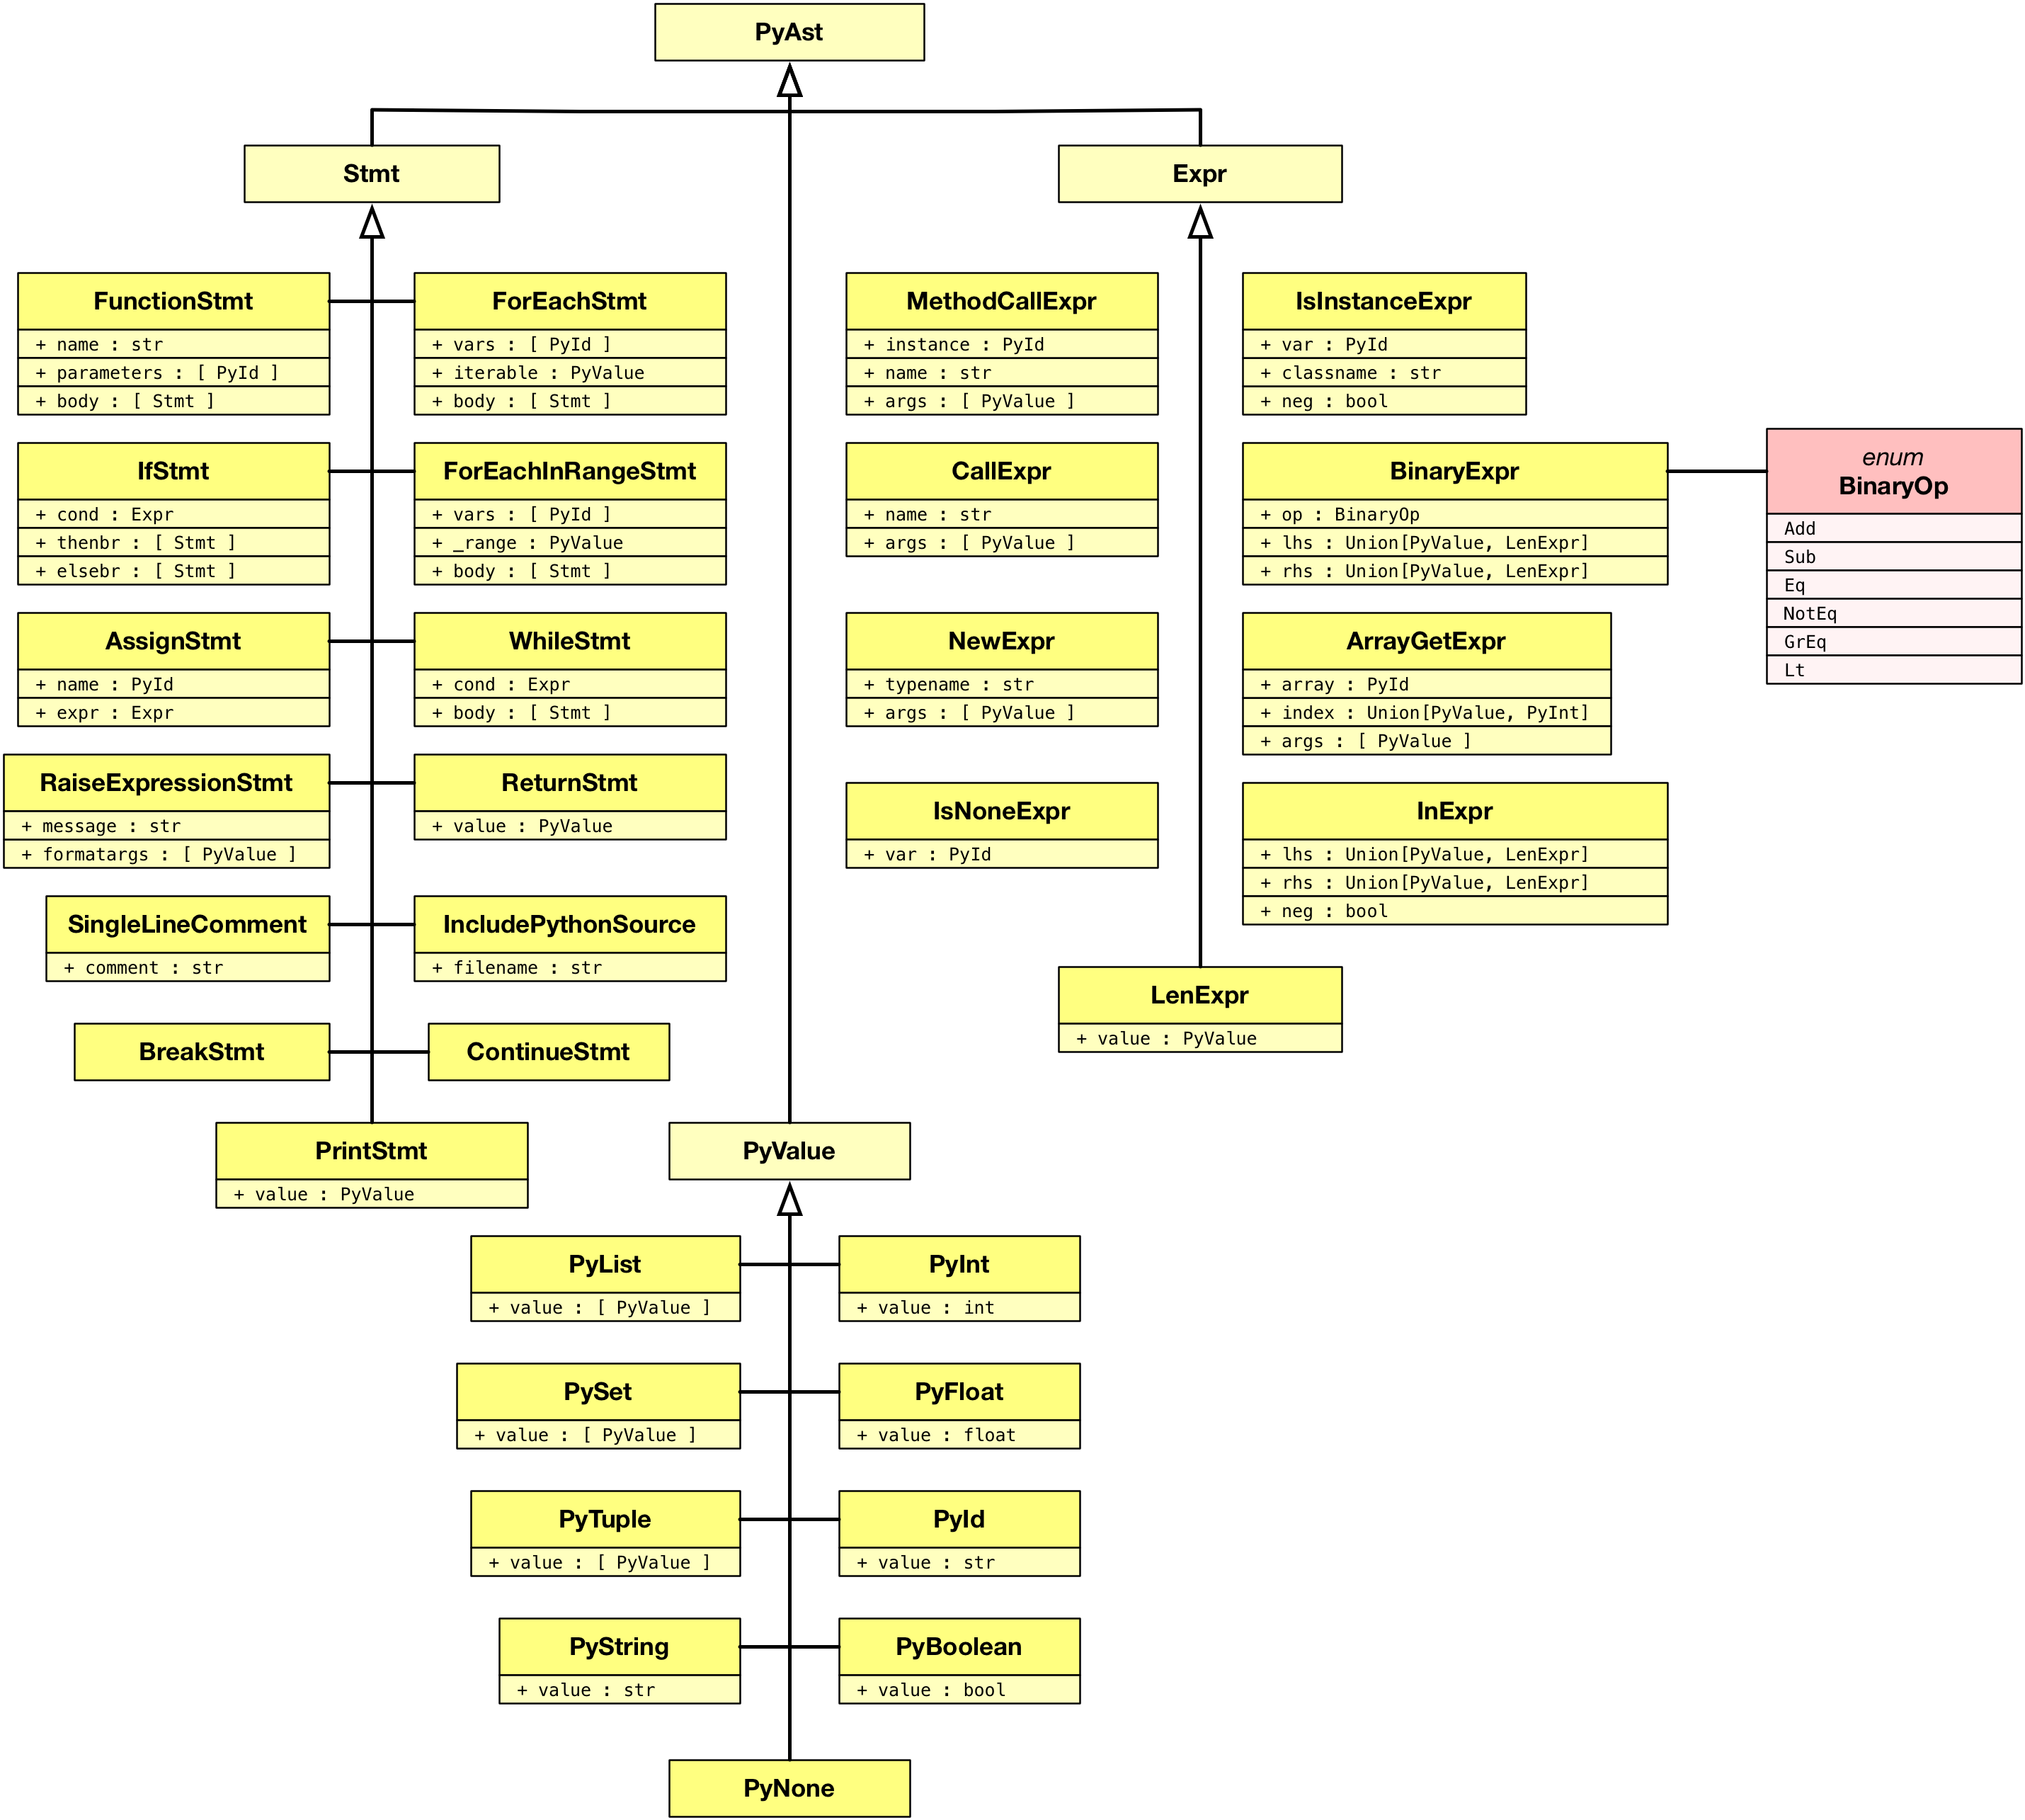
\includegraphics[scale=0.16]{class-diagram-rpython.png} }
	\caption{RPython abstract syntax tree.}
\label{class-diagram-rpython}
\end{figure}

\chapter{PyPltRedex Runtime}
\label{chapter04}

\section{Runtime Representation of Terms}
\label{section:runtime-terms}

All runtime terms are represented as shown in the class diagram in Figure \ref{class-diagram-runtime-term}

\begin{figure}[H]
	\centering
	\makebox[\textwidth][c] { 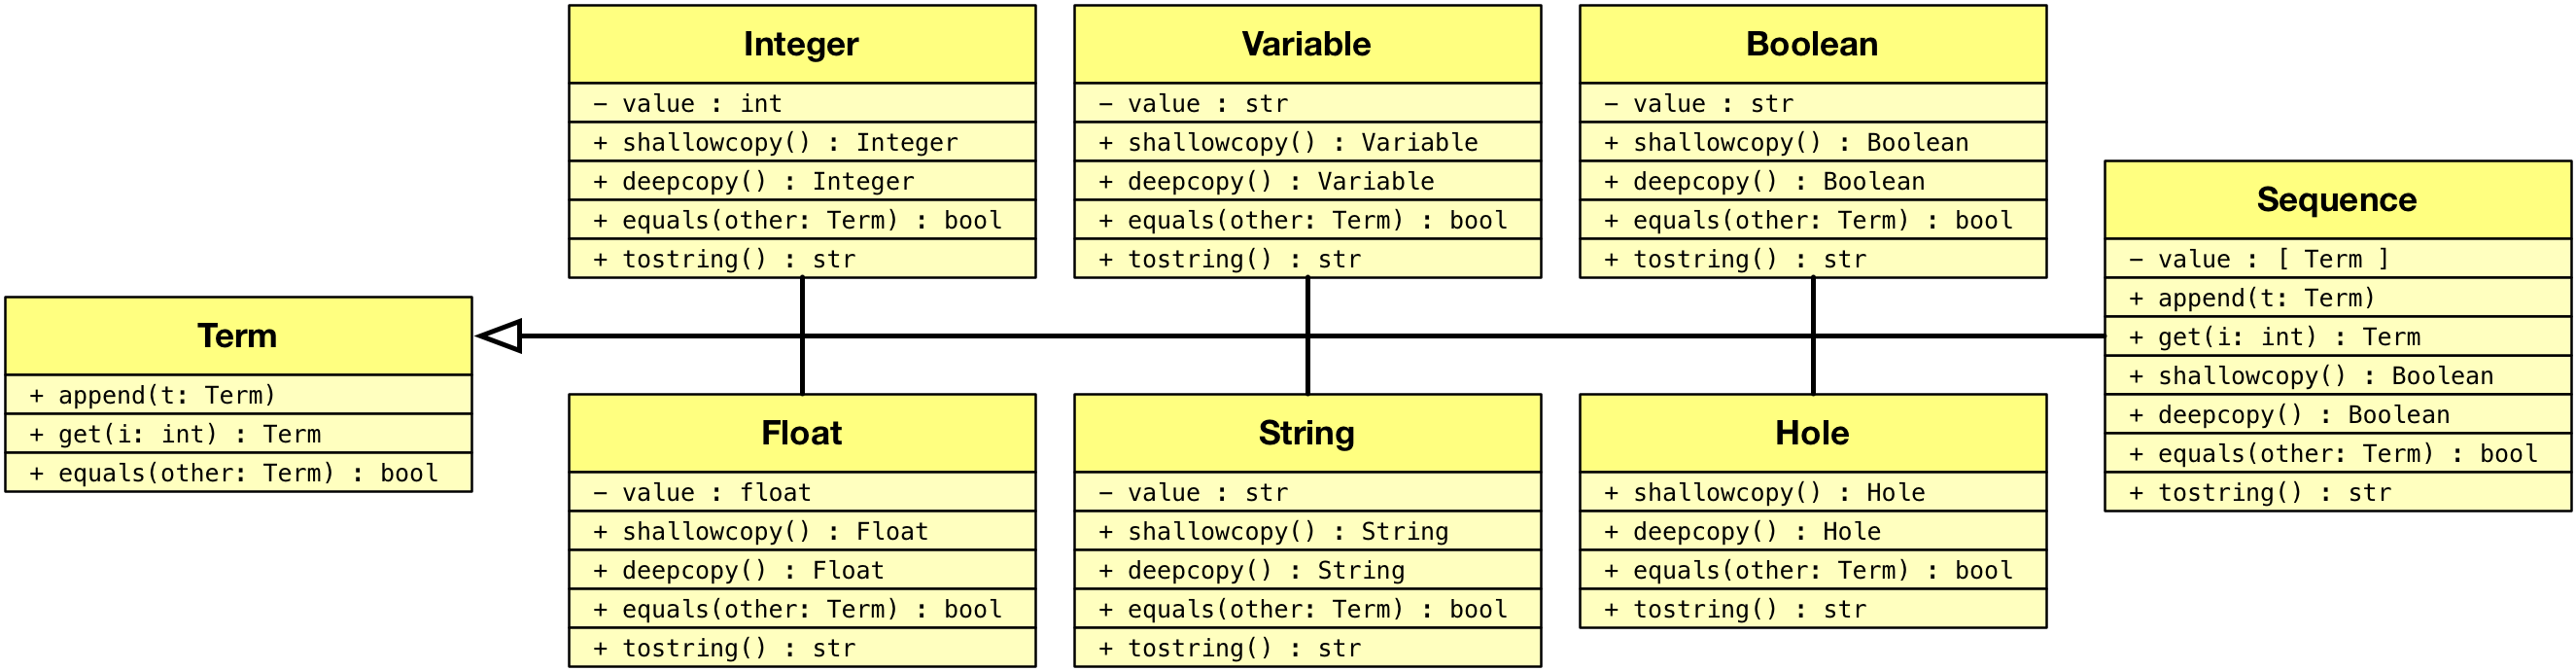
\includegraphics[scale=0.17]{class-diagram-runtime-term.png} }
\caption{\texttt{Term} class hierarchy.}
\label{class-diagram-runtime-term}
\end{figure}

These classes are all very similar and essentially just act as a wrapper for some primitive type. \texttt{Term} is the base class. Due to how RPython's type inference works creating a single class to represent all child classes such as \texttt{String} or \texttt{Float} results in the following compilation error.  Since the \texttt{LeafNode} instance is created with the \texttt{helloworld!} string, any other instantiation of \texttt{LeafNode} expects its second argument to be of type \texttt{string}. 

One may notice that, for example, \texttt{String} and \texttt{Variable} could be merged into one class and an additional \texttt{tag} field could be introduced to differentiate between strings and variables. However, since \texttt{isinstance} function is supported by RPython, such change would make term comparison logic more complex.

\begin{minted}[tabsize=2,obeytabs,fontsize=\normalsize]{python}
class LeafNode:
    def __init__(self, kind, value):
        self.kind = kind 
        self.value = value

def entrypoint():
    p = LeafNode('hello world!')
    q = LeafNode(12.5)

# UnionError:
#  SomeString(const='hello world!', no_nul=True)
#  SomeFloat(const=12.5)
\end{minted}

All classes implement the following methods.
\begin{itemize}
\item \texttt{shallow\_copy} returns an exact copy of the term. This kind of copying is not recursive.
\item
\texttt{deep\_copy} copies the term recursively. In practice, it duplicates \texttt{shallow\_copy} for every term type except \texttt{Sequence}; each term in the sequence is deep-copied and a new \texttt{Sequence} instance is returned containing copied terms.
\item
\texttt{equals} compares two terms based on the type of the term and then on the value.
\item
\texttt{tostring} returns a string representing the term. These are made to look like actual Racket expressions.
\end{itemize}
 
In addition, the following utility functions are provided to make implementation of certain functionalities easier.

\begin{itemize}
\item
	\texttt{copy\_path\_and\_replace\_last}. Given a path of terms $t_1, ..., t_n$  where terms $t_1, ..., t_{n-1}$ are expected to be of type \texttt{Sequence}, and given term $t_n^{\prime}$, the path is copied using \texttt{shallow\_copy} up to $t_n$, producing terms $t_1^\prime, ..., t_{n-1}^\prime$ and $t_n$ is replaced with $t_n^{\prime}$. All pointers to successor terms are also fixed up; that is, given two copied terms $t_i^{\prime}$ and $t_{i+1}^{\prime}$, $t_i^{\prime}$ will point to $t_{i+1}^{\prime}$ instead of $t_{i+1}$. $t_1^\prime$ is returned.
\item
	\texttt{locatehole} recursively traverses the term $t$ looking for term of type \texttt{Hole}. Each term on the path to \texttt{Hole} is recorded and upon successful search the path is returned.
\item
	\texttt{plughole}. Given two terms $t_1$ and $t_2$, first \texttt{locatehole} is called with $t_1$ as an argument. If a resulting path is non-empty, the result of \texttt{copy\_path\_and\_replace\_last} called with resulting path and $t_2$ is returned. Otherwise, $t_1$ is returned.
\item
	\texttt{asserttermsequal}. Given two terms, \texttt{equals} method is called and an Exception is raised if \texttt{equals} returns False.
\item
	\texttt{asserttermlistsequal}. Given two lists $T_1$, $T_2$ containing \texttt{Term} instances, \\ \texttt{asserttermsequal} function is called for each pair $t_1 \in T_1$ and $t_2 \in T_2$. Both lists are expected to have same lengths.
\item 
	\texttt{asserttermsequalpairwise}. Given a list $T$ containing \texttt{Term} instances, asserts that each pair $t_i, t_{i+1} \in T$ is equal, using \texttt{equals} method described previously.
\end{itemize}

\section{Runtime Representation of Matches}
\label{section:Match}

To implement matches, two classes are defined - \texttt{Match} and \texttt{Binding}, as seen in Figure \ref{class-diagram-match-binding}.

\begin{figure}[H]
	\centering
	\makebox[\textwidth][c] { 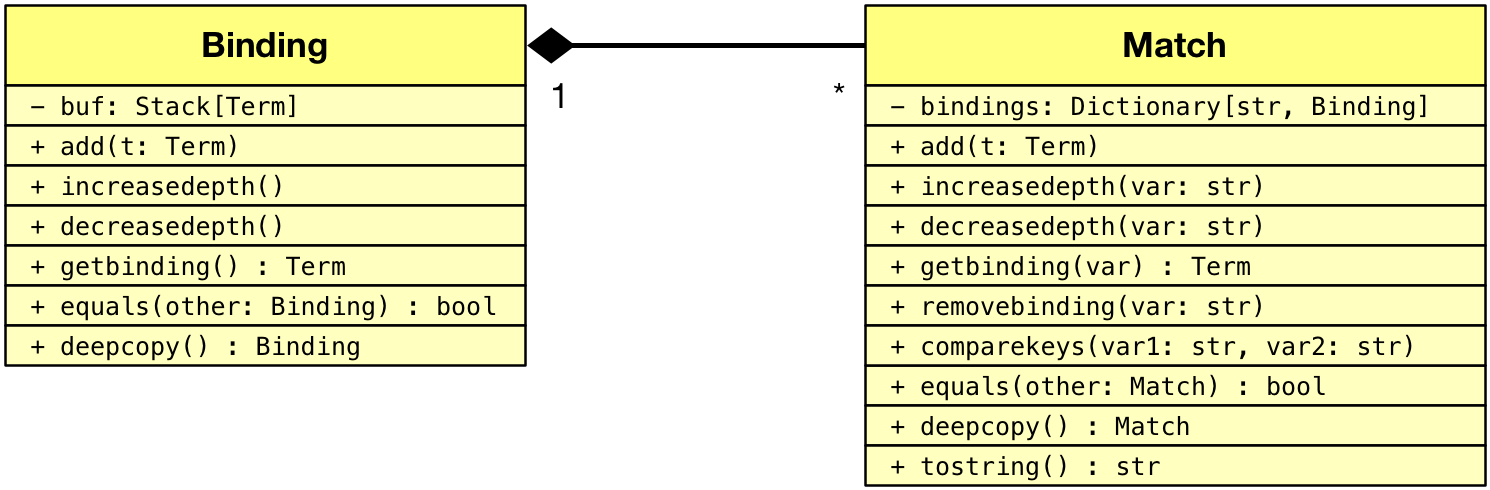
\includegraphics[scale=0.27]{class-diagram-match-binding.png} }
	\caption{\texttt{Match} and \texttt{Binding} class diagram.}
\label{class-diagram-match-binding}
\end{figure}

The \texttt{Binding} class encapsulates a stack of terms and provides three methods for its manipulation:

\begin{itemize}
\item 
\texttt{increase\_depth} pushes the term \texttt{Sequence} onto the stack provided a term on top of the stack is also a \texttt{Sequence}, otherwise it raises an Exception.

\item
\texttt{decrease\_depth} has the following behavior:
	\begin{enumerate}
		\item
        if the stack is empty, raises an Exception.
		\item
		if the stack size is 1 and the topmost element is not a \texttt{Sequence}, raises an Exception.
		\item
		if the stack size is 1 and the topmost element is a \texttt{Sequence}, does nothing.
		\item
        if the stack size is greater than one, pops the topmost \texttt{Sequence} and appends it to \texttt{Sequence} below. (this works because \texttt{increasedepth} must be called beforehand)
	\end{enumerate}

\item
\texttt{add(term)} has the following behavior:
	\begin{enumerate}
		\item
         if the stack is empty, adds \texttt{term}. 
		\item
         if the stack is not empty and the topmost term is not \texttt{Sequence}, raises an Exception
		\item
        if the stack is not empty and the topmost term is \texttt{Sequence}, adds \texttt{term} to the \texttt{Sequence}.
	\end{enumerate}
\end{itemize}

\texttt{Match} class associates pattern-variable with \texttt{Binding} instance.

\begin{itemize}
\item
\texttt{increase\_depth} calls \texttt{increase\_depth} method of relevant \texttt{Binding} instance.

\item
\texttt{decrease\_depth} calls \texttt{decrease\_depth} method of relevant \texttt{Binding} instance.

\item
\texttt{addtobinding} calls \texttt{add} method of relevant \texttt{Binding} instance with \texttt{term}.

\item
\texttt{comparekeys(key1, key2)}. Given two keys, appropriate \texttt{Binding} instances are retrieved and then the topmost terms on the stack are compared.

\item
\texttt{deepcopy} creates a new \texttt{Match} with deep-copies of \texttt{Binding} and \texttt{Term}. 
\end{itemize}

\section{Processing Input}
\label{section:lex-parse}

\subsection{Lexical Analysis and Parsing}
Since user-provided programs for a given language are initially stored as a string, it first needs to be transformed into something that could be interpreted, which in this case are \texttt{Term} instances, described in Section \ref{section:runtime-terms}. 

\begin{enumerate}
\item
\textit{Lexical analysis} breaks up the string into individual tokens and decides which kind of token it is. Most commonly tokens are described using regular expressions. 
\item 
Parsing takes individual lexemes and based on lexeme kind the appropriate \texttt{Term} instance is returned.
\end{enumerate}

However, since PLTRedex is embedded into Racket, all user-defined languages use either atoms such as integers and identifiers or potentially nested lists of atoms. The grammar for such expressions can be seen in Figure \ref{tok-lex-grammar}.

\begin{figure}[h]
\begin{minted}[tabsize=2,obeytabs,escapeinside=::,mathescape=true,fontsize=\normalsize]{text}
term = term-sequence 
     | term-atom

term-sequence = lparen term* rparen

atom = (\#true|\#false|\#t|\#f)					  :$\langle boolean \rangle$:
	   | \"([^\"\\]|(\\[\s\S]))*\"				   :$\langle string  \rangle$:
	   | (\+|\-)?[0-9]*\.[0-9]+					    :$\langle float \rangle$:
	   | (\+|\-)?[0-9]+							        :$\langle integer \rangle$:
	   | ([^ \(\)\[\]\{\}\"\'`;\#\n])*
	     ([^ \(\)\[\]\{\}\"\'`;\#0123456789\n])+ 
	     ([^ \(\)\[\]\{\}\"\'`;\#\n])*       :$\langle identifier \rangle$:

lparen = [\[\{\(]             :$\langle opening \text{ } parentheses \rangle$:
rparen = [\]\}\)]             :$\langle closing \text{ } parentheses \rangle$:
\end{minted} 
\caption{Grammar for terms. All atoms match given regular expressions.}
\label{tok-lex-grammar}
\end{figure}

\subsection{Implementation}
The class diagram for both \texttt{Tokenizer} and \texttt{Parser} can be seen in Figure \ref{class-diagram-lexer-parser}.

\begin{figure}[h]
	\centering
	\makebox[\textwidth][c] { 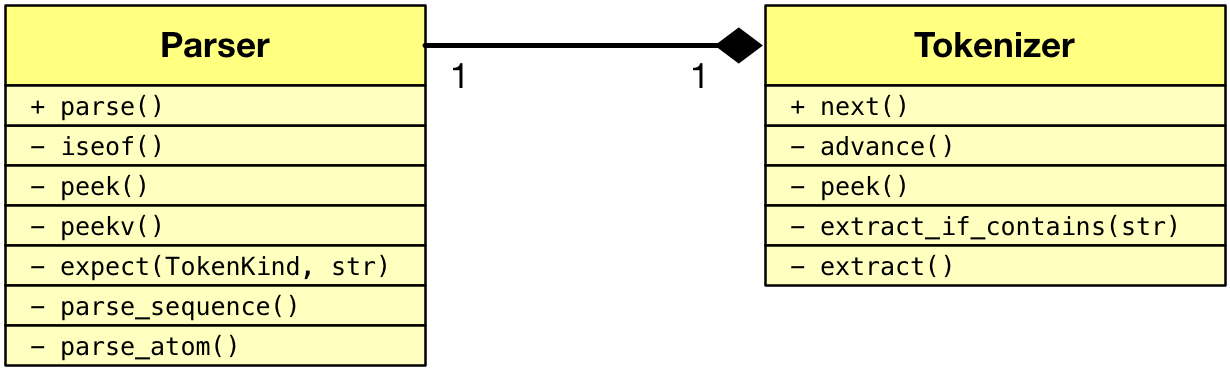
\includegraphics[scale=0.30]{class-diagram-lexer-parser.png} }
\caption{Class diagram for \texttt{Tokenizer} and \texttt{Parser}.}
\label{class-diagram-lexer-parser}
\end{figure}

The lexer implementation doesn't use regular expressions that were described above but implements their functionality using a manually implemented state machine. Functions that classify characters can be seen in Figure \ref{characterpredicates}.

\begin{figure}[h]
\begin{minted}[tabsize=2,obeytabs,escapeinside=::,mathescape=true,fontsize=\normalsize]{python}
def is_whitespace(c):
    return c == ' ' or c == '\t' or c == '\n' or c == '\r'

def is_newline(c):
    return c == '\n'

def is_reserved(c): 
    return c in ['(', ')', '[', ']', '{', '}', '\"', '\'', '`', ';', '#', '|', '\\']

def is_digit(c):
    return c in ['0', '1', '2', '3', '4', '5', '6', '7', '8', '9']

def is_plusminus(c):
    return c in ['-', '+']

def is_delimeteter(c):
    return is_reserved(c) or c == '\0' or is_whitespace(c)

def is_leftparen(c):
	return c in ['(', '[', '{']

def is_rightparen(c):
	return c in [')', ']', '}']
\end{minted}
\caption{Predicates for character identification.}
\label{characterpredicates}
\end{figure}


\begin{itemize}
\item
\texttt{string} is the string that requires lexical analysis.

\item
\texttt{start} and \texttt{end} are indices indicating an interval within the \texttt{string}. The substring that ends with the index \texttt{start} has already been analyzed. A substring between \texttt{start} and \texttt{end} is a potential token. Any substring after \texttt{end} requires analysis.

\item
\texttt{advance()} method increments \texttt{end} by one.

\item
\texttt{peek()} returns a character at index \texttt{end} of the \texttt{string}.

\item
\texttt{extract\_if\_contains(substring)} extracts substring \texttt{s} beginning at \texttt{start} and ending at \texttt{start+len(substring)} and compares it against provided \texttt{substring}. If both strings are equal, \texttt{start} and \texttt{end} indices are set to \texttt{start+len(substring)} and True is returned. Otherwise, False is returned.

\item
\texttt{extract()} extracts the string between \texttt{start} and \texttt{end}, sets \texttt{start=end} and returns the extracted string.

\item
	\texttt{next()} returns the next token in the string. This method implements the tokenization logic. All regular expressions are implemented directly instead of using RPython's regular expression library (for reasons why see below). State machine representing this method can be seen in Figure \ref{lexical-analysis-tokenize}.

\begin{figure}[th!]
	\centering
	\makebox[\textwidth][c] { 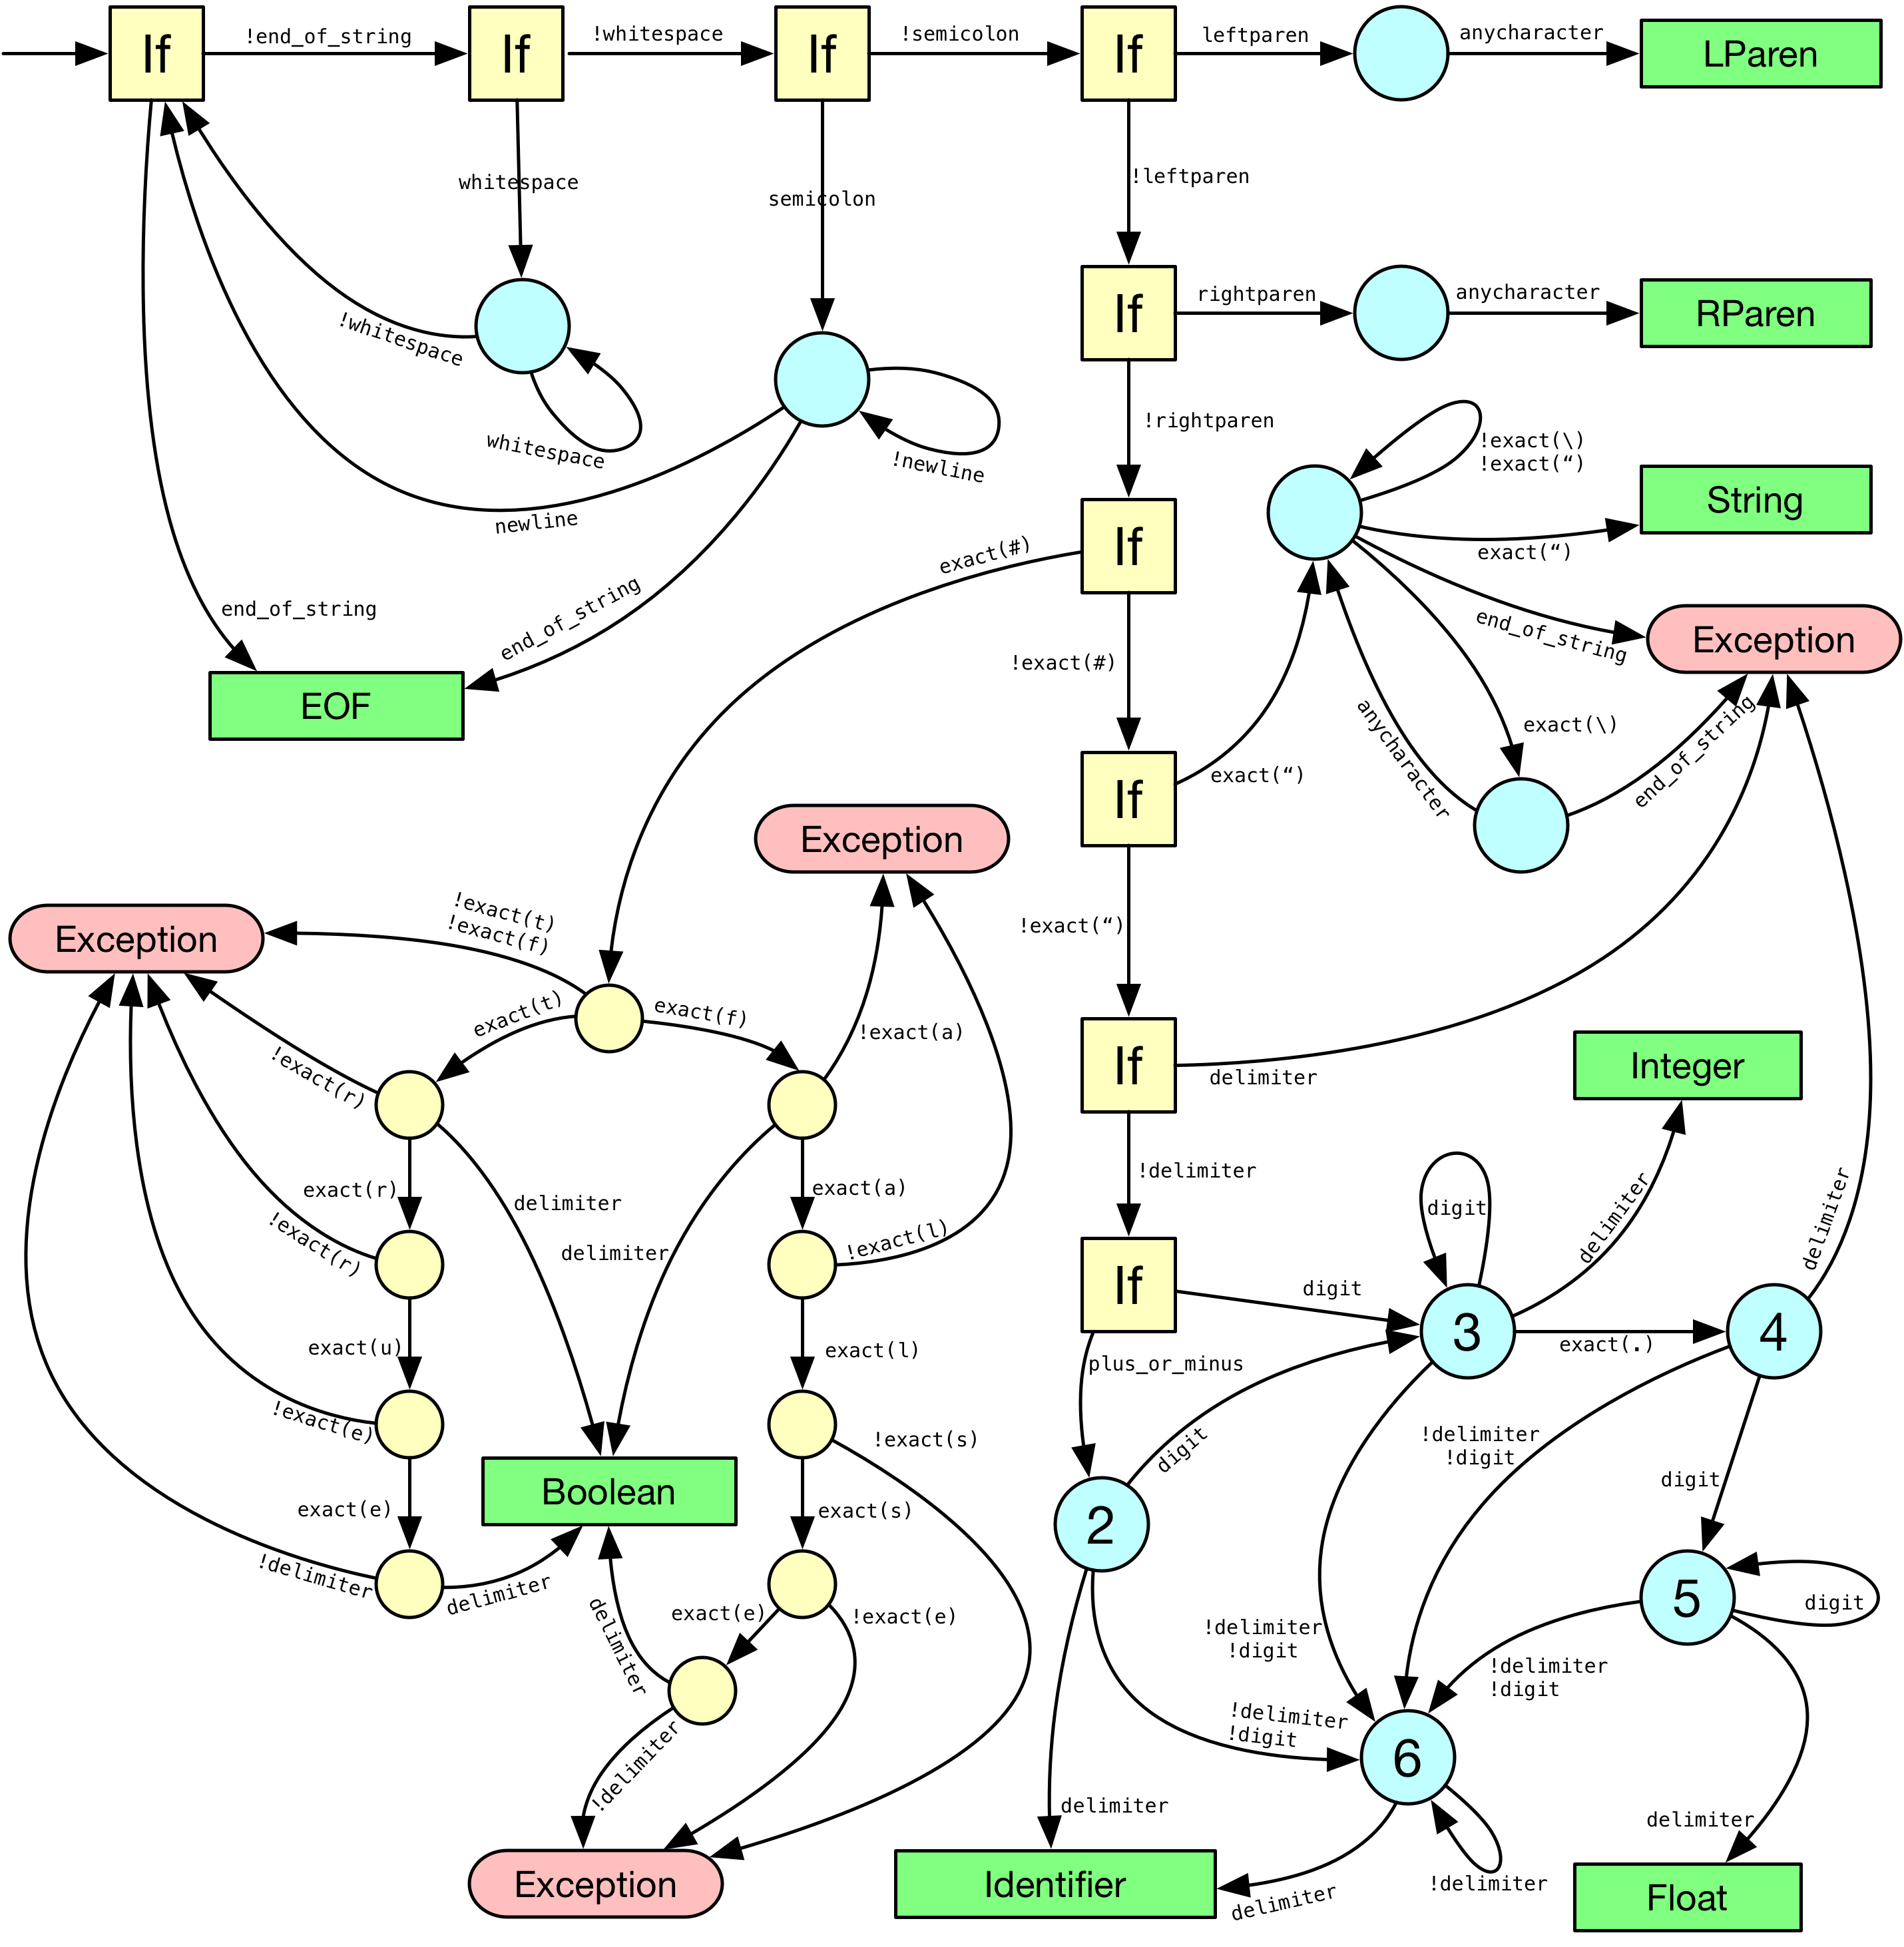
\includegraphics[scale=0.16]{lexical-analysis-tokenize.png} }
\caption{State machine for lexical analysis.}
\label{lexical-analysis-tokenize}
\end{figure}

Edges of the graph represent calls to \texttt{peek()} and ensures the character satisfies a predicate that an edge is labeled with (see Figure \ref{characterpredicates}). Unlike more traditional state machines such as finite automatons (in which moving from one state to another is associated with input consumption), the one above consumes input only after switching to some state. There are different state kinds which consume input in different ways.
\begin{itemize}
\item States that return tokens annotated with their types are highlighted in green. After moving to this state no input is consumed.
\item States that raise Exceptions are highlighted in red. After moving to this state no input is consumed.
\item \texttt{If} states correspond to \texttt{if} statements. They consume no characters.
\item Circled blue states actually consume characters that satisfy a predicate that the incoming edge is labeled with. They can also have self-loops indicating consumption of one or more characters satisfying a given predicate.
\item Circled yellow states are conceptually identical to blue states but are handled differently as explained below.
\end{itemize}

The state machine proceeds in the following manner:

\begin{enumerate}
\item First it ensures the end of the string has not been reached, otherwise \texttt{EOF} token is returned. 
\item Then, if the current character is whitespace, greedily consume all whitespace characters and move to initial state.
\item If the current character is a semicolon thus indicating the beginning of a comment, greedily consume all characters until a newline character or end of the string, thus returning \texttt{EOF} token. 
\item The next two \texttt{If} statements detect opening and closing parentheses/braces/brackets and return \texttt{LParen} or \texttt{RParen} tokens accordingly.
\item If the current character starts with a pound sign indicating a possible boolean, the transition to the yellow state would be taken. However, these yellow states do not consume input on character by character basis like blue states do but utilize \texttt{extract\_if\_contains} method to peek and consume multiple characters at once. This method is called in the following manner:
\begin{itemize}
\item
if \texttt{extract\_if\_contains("\#t")} return \texttt{(Boolean, \#t)}
\item
if \texttt{extract\_if\_contains("\#f")} return \texttt{(Boolean, \#f)}
\item
if \texttt{extract\_if\_contains("\#true")} return \texttt{(Boolean, \#t)}
\item
if \texttt{extract\_if\_contains("\#false")} return \texttt{(Boolean, \#f)}
\end{itemize}

\item If the current character is a double quote, consume any character until the closing double quote is found. Escape sequences are supported expecting a single character after a backward slash. If end-of-string is encountered prematurely, an Exception is raised. Otherwise, a \texttt{(String, self.extract())} token is returned.

\item Finally, the only token kinds remaining to process are \texttt{Integer}, \texttt{Float} and \texttt{Identifier}. First, need to ensure that the current character is not a special reserved one, raising an Exception. Otherwise, state machine moves to the last \texttt{If} statement. Essentially, the state machine attempts to match an \texttt{Integer} or \texttt{Float} first but once a character that may not be in these two token kinds is seen, the resulting token immediately becomes \texttt{Identifier}. All input from that point on is consumed greedily until some delimiter character.
\end{enumerate}

\end{itemize}

This completes the description of the \texttt{Tokenizer}. The parser is implemented as a very simple recursive descent parser. Below follows the description of its methods and their functionalities.

\begin{itemize}
\item
\texttt{iseof()} returns true if the end of the string has been reached.

\item
\texttt{peek()} returns kind of the next token. 

\item
\texttt{peekv()} returns kind of the next token along with its value.

\item 
\texttt{expect(expectedkind, tok=None)} throws Exception when \texttt{currenttoken} is not the one expected. In particular:
	\begin{itemize}
		\item
		If \texttt{expectedkind != nexttoken.kind}, raise an Exception.
		\item
		If \texttt{tok != None}, check if \texttt{tok=nexttoken.value} and raise an Exception if it is not.
		\item
		Otherwise, call \texttt{tokenizer.next()} and assign it to \texttt{nexttoken} and return the previous token. 
	\end{itemize}

\item 
	\texttt{parse\_sequence} implements parsing of \texttt{term-sequence} from the grammar above
	\begin{itemize}
		\item
		Let \texttt{seq} be an empty list.

		\item
		The first token is expected to be \texttt{LParen}.

		\item
		While \texttt{peek()} is not \texttt{RParen}, if \texttt{peek()} is \texttt{LParen}, call \texttt{term-sequence} and append its result to \texttt{seq}, otherwise call \texttt{parse\_atom} and append its result to \texttt{seq}.
	
		\item
		\texttt{expect(RParen)} and return \texttt{Sequence(seq)}
	\end{itemize}

\item
\texttt{parse\_atom} implements parsing of \texttt{atom} from grammar.
	\begin{itemize}
	\item
		If \texttt{peek()} is an \texttt{Integer} token, return \texttt{Integer(expect(Integer))}
	\item
		If \texttt{peek()} is a \texttt{Float} token, return \texttt{Float(expect(Decimal))}
	\item

		If \texttt{peek()} is a \texttt{String} token, return \texttt{String(expect(String))}
	\item
		If \texttt{peek()} is a \texttt{Boolean} token, return \texttt{Boolean(expect(Boolean))}
	\item

		If \texttt{peek()} is an \texttt{Ident} token, then call \texttt{peekv} to retrieve the \texttt{value} of the token. If a \texttt{value} of token is \texttt{hole} return \texttt{Hole()}, otherwise \texttt{Variable(value)} is returned
	\end{itemize}
	

\end{itemize}

\subsection{Implementation: Difficulties}
The implementation of the initial lexical analysis relied on a regular expression library provided by RPython used to identify integers, floating point numbers, and identifiers using regular expressions shown in Figure \ref{tok-lex-grammar}. While the library works fine when running the lexer using \texttt{python2.7}, attempting to compile the lexer code using \texttt{rpython} toolchain results in the following compilation error:

\begin{minted}[tabsize=2,obeytabs,fontsize=\normalsize]{python}
[translation:ERROR] AttributeError: 'FrozenDesc' object has no attribute 'pycall'
Processing block:
 block@1149[_choice5_0...] is a <class 'rpython.flowspace.flowcontext.SpamBlock'> 
 in (rpython.rlib.parsing.regexparse:1495)RegexParser._charclass 
 containing the following operations: 
       v1 = simple_call((type set), v0) 
       v2 = simple_call((builtin_function range), (97), (123)) 
       v3 = newlist() 
       v4 = iter(v2) 
       v5 = hint(v3, v2, ({'maxlength': True})) 
\end{minted}

There appears to be a bug within RPython's \texttt{RegexParser} functionality. After investigating the issue, it was decided to implement these regular expressions manually instead of relying on the library. This decision was also made because the construction of those regular expressions was rather slow.

\subsection{Future Improvements}

Since lexical analysis and parsing were implemented very early on, some of the regular expressions were hacked together to make everything work in short amount of time. In certain cases tokenization is not performed correctly with respect to Racket's tokenization logic. For example, Racket allows for the specification of floating point numbers such as \texttt{.045} or \texttt{1.} (that is there must be either a digit before or after a decimal), which the current implementation doesn't support (and are identified as Identifier instead). Scientific notation isn't supported, either.

\section{Fresh Variable Generation}
PLTRedex provides a very convenient form \texttt{(variables-not-in t p)}. Term \texttt{p} is expected to contain a single variable \texttt{v} such as \texttt{(term a)}. Given term \texttt{t}, \texttt{variables-not-in} form produces a term containing a fresh variable \texttt{v\_out} with prefix \texttt{p\_out} and some suffix \texttt{s\_out} such that there's no variable \texttt{v\_prime} in \texttt{t} with \texttt{v\_out = v\_prime}; or \texttt{v\_out not in Variables(t)} where \texttt{Variables(t)} is the set of all variables in \texttt{t}. Suffix \texttt{s\_out} may contain only digits or be empty. 

For example, variable \texttt{abc1xyz123} is decomposed into prefix \texttt{abc1xyz} and suffix \texttt{123}.

\subsection{Algorithm}
\begin{itemize}
\item
Initialize an empty dictionary.

\item
For each \texttt{v\_prime in Variables(t)}, try to decompose \texttt{v\_prime} into \texttt{p\_prime} and \texttt{s\_prime} interpreted as a number. 

	\begin{itemize}
	\item
	If such decomposition is possible, insert \texttt{(p\_prime, s\_prime)} into the dictionary. If \texttt{p\_prime} is not in the dictionary, initialize it to be an empty list and append \texttt{s\_prime} to it.

	\item
		Otherwise, insert \texttt{(v\_prime, -1)} into the dictionary \texttt{d}. If \texttt{v\_prime} is not in the dictionary, initialize it to be an empty list and append string -1 to it. A special value of -1 is used to indicate that \texttt{v\_prime} does not have a suffix.
	\end{itemize}

\item
Decompose \texttt{v} into prefix \texttt{p} and suffix \texttt{s}.

	\begin{itemize}
	\item
	If decomposition is not possible, check if \texttt{v} is in dictionary \texttt{d} and if it isn't return \texttt{Variable(v)}, meaning term \texttt{v} is not in \texttt{Variables(t)}.
	\item
	If decomposition is possible, check if \texttt{p} is in dictionary \texttt{d} and if it isn't return \texttt{Variable(v+s)}. Additionally, check if suffix \texttt{s} is in \texttt{d[p]}. If it isn't, return \texttt{Variable(v+s)}. This is done to return \texttt{a00} given \texttt{Variables(t) = \{a, a0\}} and \texttt{v=a00}, for example. Otherwise, let \texttt{v=p}.
	\end{itemize}

\item
Otherwise, the algorithm searches for a unique suffix by interpreting each suffix in \texttt{d[v]} as a number. Let \texttt{N} be the list containing prefixes interpreted as a number and sorted in ascending order.  The goal is to find the smallest number \texttt{i > 0} that is not in \texttt{N}. If first \texttt{N[0]} is not \texttt{-1}, then \texttt{v} is not in \texttt{Variables(t)} and is already fresh. Return \texttt{Variable(v)}.

\item
Initialize \texttt{i=1} and \texttt{j=1}. \texttt{N[0]} is -1. Let \texttt{n} be the length of the list \texttt{N}. While \texttt{j<n}:
	\begin{itemize}
		\item
		If \texttt{i < N[j]} return \texttt{Variable(v+i)}.
		\item
		If \texttt{i > N[j]} then increment \texttt{j} by one. This case only happens when 0 is in \texttt{N}.
		\item
		If \texttt{i = N[j]} then increment both \texttt{i} and \texttt{j} by 1.
	\end{itemize}
\item
The end of the list is reached and \texttt{Variable(v+i)} is returned.
\end{itemize}






\chapter{Compile-Time PLT Redex Representation}
\label{chapter05}

This chapter describes how PyPltRedex represents the constructs of PLTRedex that were described in Section \ref{01-pltredex} and establishes the notation that will be used throughout the report. Forms that are not part of PLTRedex are also introduced.

\section{Pattern Language}

This section describes the subset of PLTRedex's pattern specification language supported by \texttt{PyPltRedex}. Grammar for the pattern language can be seen in Figure \ref{pattern-grammar}, in EBNF notation. 

\begin{figure}[h]
\begin{minted}[tabsize=2,obeytabs,escapeinside=//,mathescape=true,fontsize=\normalsize]{text}
pattern = number 
        | integer 
        | real 
        | natural 
        | string 
        | boolean 
        | variable-not-otherwise-mentioned 
        | hole 
        | symbol
        | (in-hole pattern pattern)
        | (pattern-sequence *) 

pattern-sequence : pattern 
                 | pattern ...  # literal ellipsis
\end{minted}
\caption{Grammar of the pattern language.}
\label{pattern-grammar}
\end{figure}

\begin{itemize}
\item
\textit{number} pattern matches any number.

\item
\textit{integer} matches any exact integer. 

\item
\textit{real} matches any real number.

\item
\textit{natural} matches any natural number; that is, any non-negative integer.

\item
\textit{string} matches any string.

\item
\textit{boolean} matches any boolean \texttt{\#t} or \texttt{\#f}.
\item
\textit{variable-not-otherwise-mentioned} matches any symbol that is not used as a literal in the language definition. For example, if language definition contains the pattern \texttt{(+ number number)} \textit{variable-not-otherwise-mentioned} will not match symbol \texttt{+}.

\item
\textit{hole} matches \texttt{hole} term exactly.

\item
\textit{symbol} matches any symbol except if its value coincides with non-terminal symbol in the language definition or contains an underscore.
\end{itemize}

All patterns above, except \textit{hole} can be suffixed with underscore and identifier (for example, \textit{number\_1}) to create a binding to a matched term.

\begin{itemize}
\item
\textit{(in-hole pattern pattern)} traverses the term trying to match the second pattern; upon successful match the term matching the second pattern is replaced with the term \texttt{hole} and then the first pattern is matched. The first pattern must match exactly one hole.

\item
\textit{pattern-sequence} pattern matches a term list, where each pattern-sequence element matches an element of the list. Each individual pattern within the sequence can be suffixed with \texttt{...} (literal ellipsis) and that will match zero or more terms matching the pattern.

Ellipses may produce non-deterministic matches. For example, consider a pattern \texttt{(number\_1\ ...\ number\_2\ ...)} and a term \texttt{(1 2)}. There are three resulting matches: 
\begin{itemize}
	\item \texttt{(number\_1:\ (), number\_2:\ (1 2))}
	\item \texttt{(number\_1:\ (1), number\_2:\ (2))}
	\item \texttt{(number\_1:\ (1 2), number\_2:\ ())}
\end{itemize}
		
In the first case, \texttt{number\_1 ...} matches zero terms that match the pattern \texttt{number\_1} and hence pattern \texttt{number\_2\ ...} has to match remaining numbers. In the second case, \texttt{number\_1\ ...} matches a term \texttt{1}, and hence the term \texttt{2} is matched by \texttt{number\_2 ...}. Lastly, \texttt{number\_1\ ...} may match all the numbers in the sequence, leaving nothing for \texttt{number\_2\ ...} to consume.
\end{itemize}

If patterns in the pattern-sequence are suffixed with the same identifier (e.g. \texttt{(number\_1 number\_1)})), then the match is constrained to terms that are equal. That means term \texttt{(1 1)} matches the pattern but \texttt{(1 2)} does not. For patterns in a \texttt{define-language} form constraint checking is not performed. PLTRedex provides other constraint checks but they will not be considered.

\section{Compile-Time Representation of Patterns}

Throughout the report the following notation will be used to represent the Python classes used in the implementation of the pattern language. It follows the following format: \mintinline{text}{Typename(|$a$|: A, [|$b_1,...,b_n$|]: B, [|$c_1,...,c_m$|]: C?)}. $a$ is a field of type \texttt{A}. \mintinline{text}{[|$b_1,...,b_n$|]} is a sequence containing $n$ fields of type \texttt{B}. \mintinline{text}{[|$c_1,...,c_m$|]} is a sequence containing \textit{zero} or $m$ fields of type \texttt{C} (that is, \texttt{C?} is an optional type).

\begin{figure}[ht]
	\centering
	\makebox[\textwidth][c] { 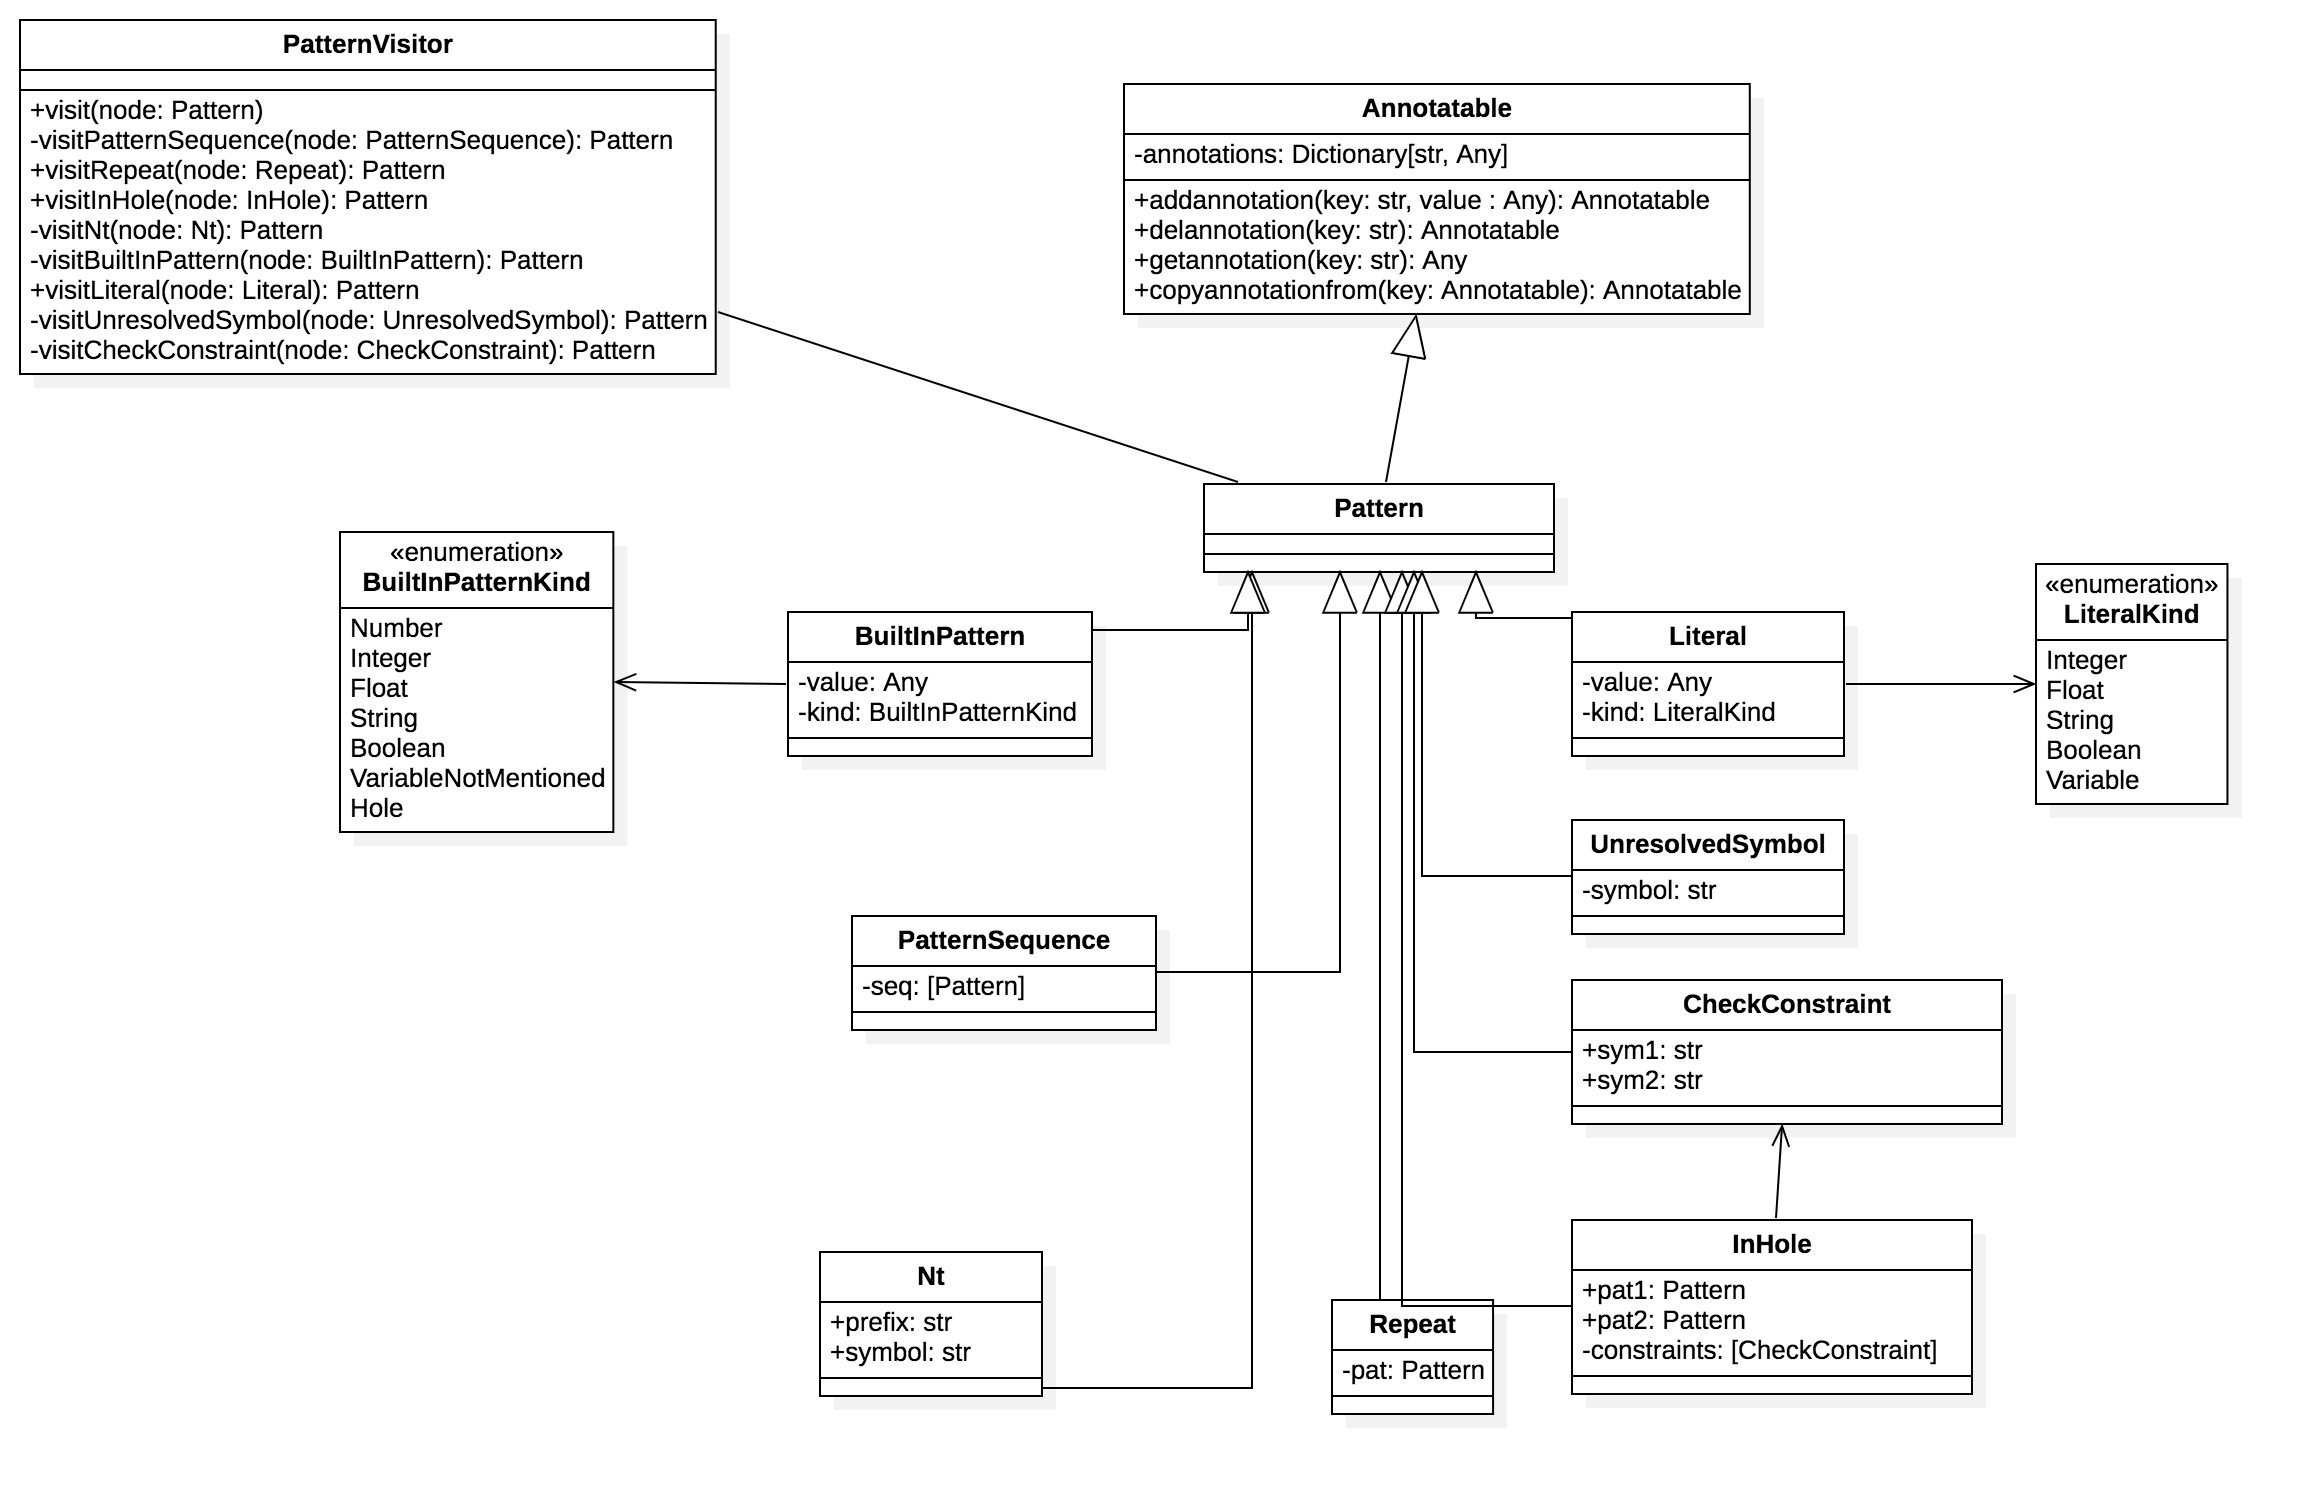
\includegraphics[scale=0.23]{class-diagram-pattern.png} }
	\caption{Representation of patterns.}
\label{class-diagram-pattern}
\end{figure}

Figure \ref{class-diagram-pattern} shows class diagram for all patterns.

\begin{itemize}
\item
\PatternSequence \space represents the \texttt{pattern-sequence} clause of the pattern language and may contain zero or more child patterns $p_i$. 

\item 
\PatternRepeat \space represents pattern $p_r$ under ellipsis.

\item
\PatternCheckConstraint is used for equality checking of terms. Terms assigned to $sym_1$ and $sym_2$ are checked for equality.

\item 
\NonTerminal \space represents non-terminal. $nt$ is a non-terminal symbol, while $pv$ is a pattern-variable to which some term will be assigned during matching. 

\item
\BuiltInPattern \space represents various built-in patterns such as \texttt{number} or \texttt{string}. $tag$ is chosen from \texttt{BuiltInPatternKind} enumeration.

\item
\PatternInHole \space represents \texttt{in-hole} pattern where $p_1$ and $p_2$ are patterns, and $c_1, ..., c_n$ are optional \ConstraintCheckNoArg \space instances.

\item 
\LiteralPattern \space represents a literal value seen in a pattern. Its $kind$ is chosen from \texttt{PatternLiteralKind} enumeration and $v$ is the value of the literal. The type of the literal must match the $kind$.

\item 
\UnresolvedSymbol is used to represent symbols that are initially unknown to be non-terminal, built-in pattern, or literal; $sym$ is the symbol.

\end{itemize}

\section{Term-Templates}
\label{section:term-templates}

The compile-time representation of terms differs greatly from the runtime representation described previously. The reason for this is the necessity to handle ellipses; or, more specifically, the substitution of pattern variables under ellipses - \texttt{PLTRedex} handles this dynamically and erroneous ellipses aren't detected until term creation time.
It is desirable to handle ellipsis depth checking of pattern variables at compile time to be able to provide compile time error messages. Doing this allows for the complete elimination of ellipses from the runtime (with variable \texttt{...} being a reserved symbol that throws an Exception). In addition, this also allows for the detection of metafunction applications statically.

The grammar for terms can be seen in Figure \ref{termtemplate-grammar}. To differentiate between runtime terms, the compile-time representation of terms will be called \textbf{term-templates}.

\begin{figure}
\begin{minted}[tabsize=2,obeytabs,escapeinside=//,mathescape=true,fontsize=\normalsize]{text}
term-template = pattern-variable
              | (term-sequence *)
              |,(functionname term*)
              |(in-hole term term)
              | hole
              | integer
              | float
              | string
              | boolean
term-sequence = term
              | term ... ; literal ellipsis
              | ,@(function term *)
\end{minted}
\caption{Grammar for term-templates.}
\label{termtemplate-grammar}
\end{figure}

\begin{itemize}
\item
\texttt{pattern-variable} represents pattern variables.
\item
\texttt{,(functionname term*)} calls a user-implemented RPython function with zero or more terms as arguments.
\item
\texttt{,@(functionname term*)} calls a user-implemented RPython function with zero or more terms as arguments that must return a list. The content of the returned list are then inserted into term-sequence at that position.
\item
\texttt{(in-hole term term)} locates \lstinline{hole} in the first term and replaces it with the second term.
\item
\texttt{hole} represents the term \lstinline{hole}
\item
\texttt{integer} represents any literal integer.
\item
\texttt{float} represents any literal floating point number.
\item
\texttt{string}  represents any literal string.
\item
\texttt{boolean}  represents any literal boolean.
\item
	\texttt{term-sequence} represents a list of term-templates.  Each individual term-template within the sequence can be suffixed with \texttt{...} (literal ellipsis) indicating the ellipsis depth of some pattern-variable in that term-template.
\end{itemize}

\section{Compile-time Representation of Term-Templates}

Throughout the report the following notation will be used to represent actual Python classes used to implement the term-templates.

\begin{figure}[ht]
	\centering
	\makebox[\textwidth][c] { 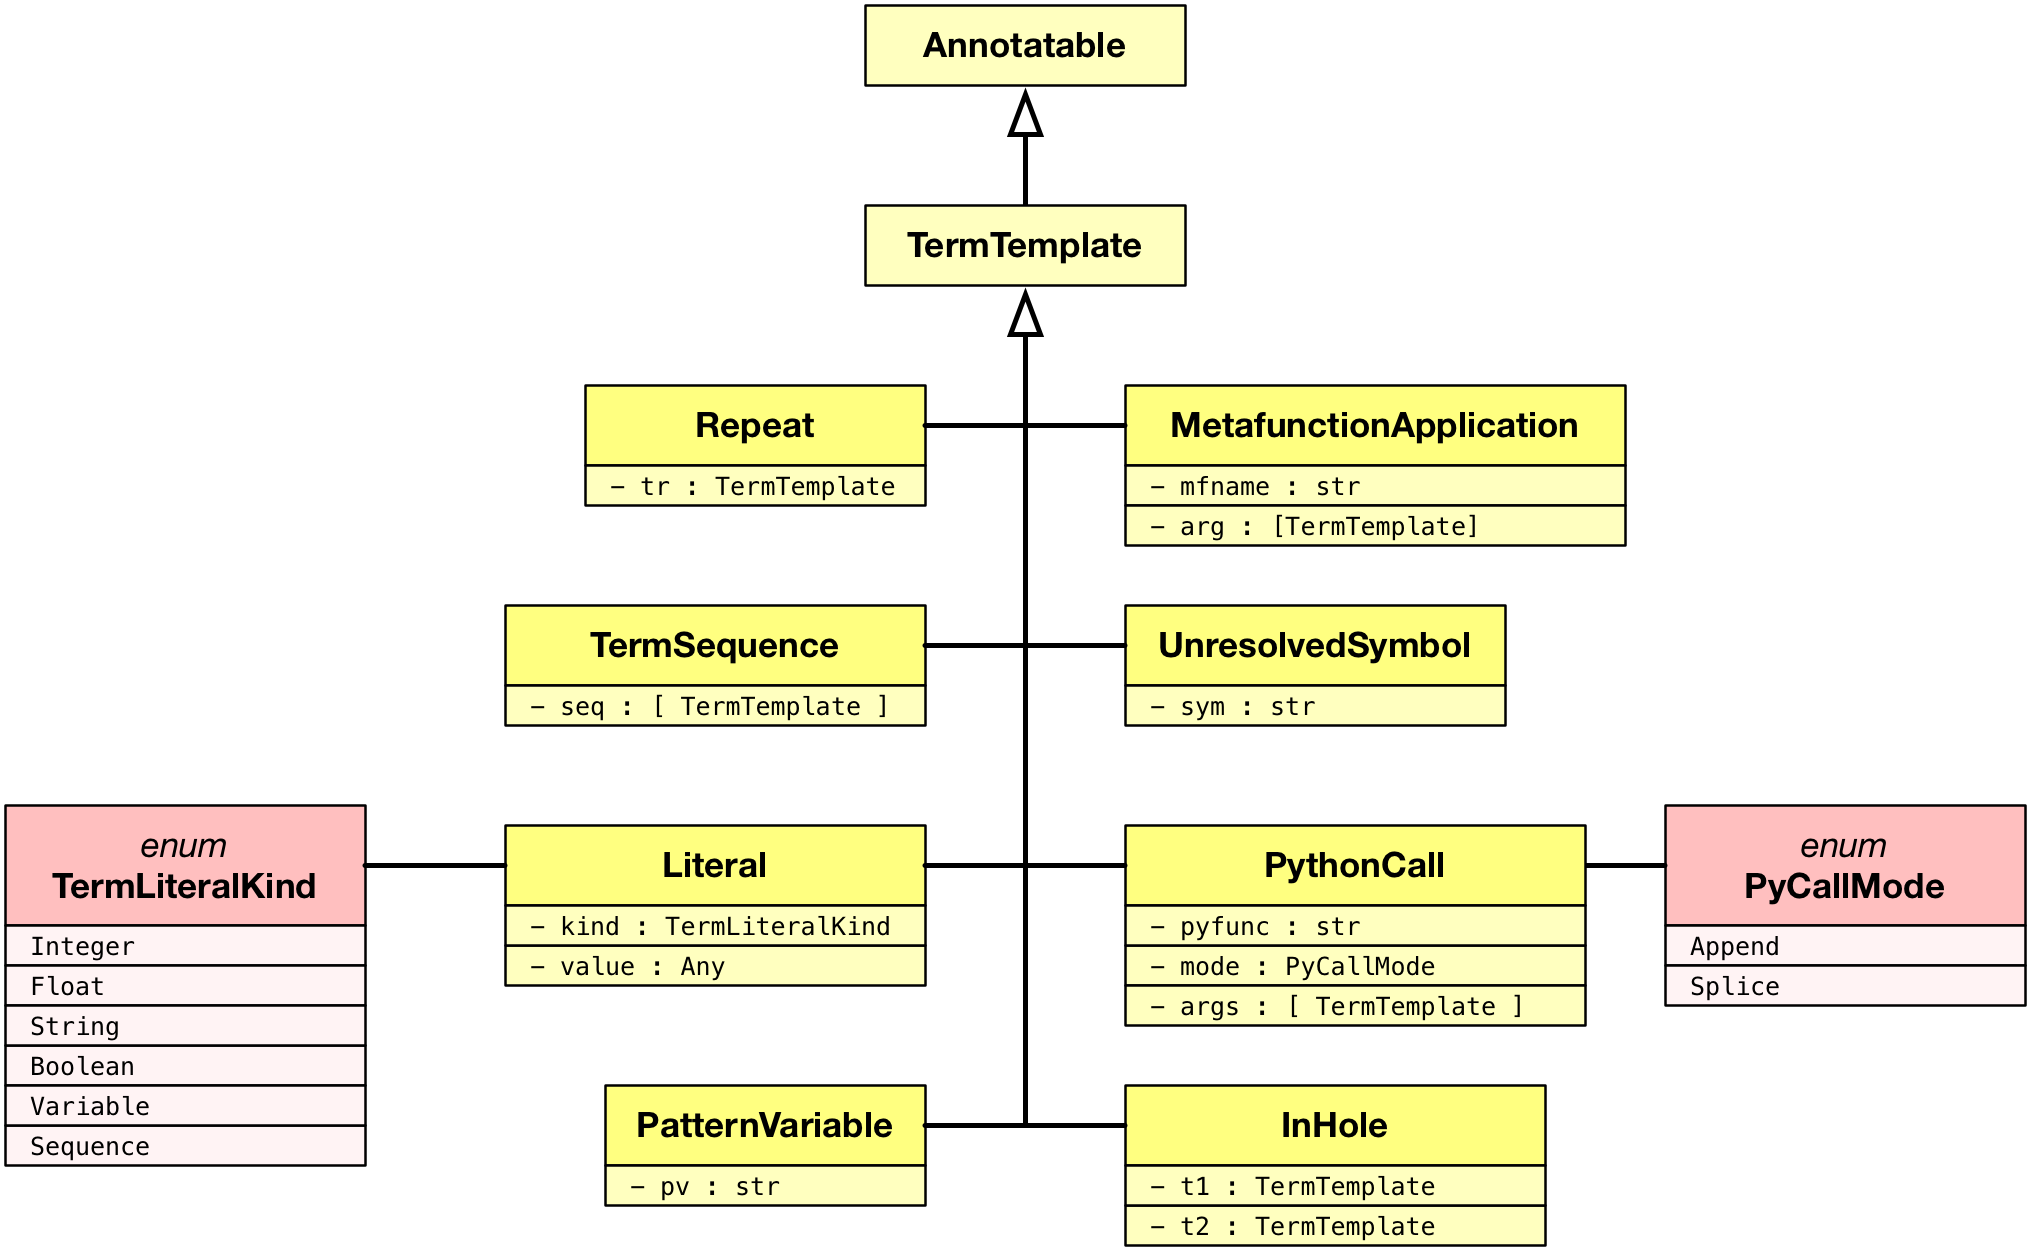
\includegraphics[scale=0.19]{class-diagram-termtemplate.png} }
	\caption{Representation of term-templates.}
\label{class-diagram-termtemplate}
\end{figure}

Figure \ref{class-diagram-termtemplate} shows class diagram for all term-templates.


\begin{itemize}
\item \TermSequence \space represents term-template sequences and may contain zero or more child term-templates $t_i$.
\item \TermRepeat \space represents a term-template under ellipsis.
\item \TermInHole \space represents \texttt{in-hole} term-template
\item \PythonCall \\ represents \texttt{,(functionname term*)} and \texttt{,@(functionname term*)} term-template. $mode$ is used to indicate which one of those it is - $m$ is set to \texttt{Normal} if it is the first, otherwise \texttt{Splice} if it is the latter. $pyfunc$ is expected to be a defined RPython-compatible function.
\item \TermLiteral \space represents any literal. It is initialized with the appropriate tag.
\item \PatternVariable \space represents all pattern-variables.
\item \UnresolvedSymbol \space represents unresolved symbols. Initially it is unknown if a symbol is a pattern-variable or a literal.
\end{itemize}

\section{Top-Level Forms}

\mbox{PyPltRedex supports three primary forms. \texttt{define-language} and \texttt{define-metafunction}} forms are lifted directly PLTRedex. \texttt{reduction-relation} form had to be modified resulting in \texttt{define-reduction-relation}. \texttt{read-from-stdin-and-apply-reduction-relation*} form  is based on  \texttt{apply-reduction-relation} but instead it reads a term from standard input, parses it, and only then applies reduction relation. The grammar for these forms can be found in Figure \ref{grammar-tlmain}.

\begin{figure}
\begin{minted}[tabsize=2,obeytabs,escapeinside=//,mathescape=true,fontsize=\normalsize]{text}
define-language = ( define-language language-name non-terminal-definition+ )
non-terminal-definition = ( non-terminal-name ::= pattern+ )

define-metafunction = ( define-metafunction language-name metafunction-contract metafunction-case+ )
metafunction-contract =	id : pattern-sequence* -> pattern
metafunction-case =  [( name pattern* ) term-template]

reduction-relation = ( define-reduction-relation name language domain reduction-case+ )
reduction-case = (-> pattern term-template reduction-case-name)
domain = #:domain pattern

read-from-stdin-and-apply-reduction-relation = ( read-from-stdin-and-apply-reduction-relation :#mf metafunction-name )
\end{minted}
\caption{Grammar for primary top-level forms.}
\label{grammar-tlmain}
\end{figure}

\begin{itemize}
\item
\TlDefineLanguage. $n$ is the name of the language and $nt_1,...,nt_m$ are \NtDefinitionN \space instances containing one or more \texttt{Pattern} instances.

\item
\TlDefineMetafunction. $n$ is the \texttt{id} specified by \texttt{metafunction-contract}. Let $p_1, ..., p_n$ be the pattern sequence specified by the \texttt{metafunction-contract}, between \texttt{id} and \texttt{->}. $domain$ pattern is then constructed in the following way: \mintinline{text}{PatternSequence(|$n$|, [|$p_1$|, |$...$|, |$p_n$|])}. $codomain$ pattern is the one following \texttt{->}. If input term doesn't match pattern $domain$, an Exception is raised. Similarly, if the resulting term doesn't match $codomain$ pattern, an Exception is also raised. If metafunction produces no terms, an Exception is raised. $mc_1,...,mc_n$ is the sequence of \space \MetafunctionCase \space containing the pattern $p$ to be matched and the term-template $t$ to plug matches into. $l$ is the name of the language with respect to which all non-terminal symbols in patterns $p$ are resolved.

\item \TlDefineReductionRelation. $n$ is the name of the reduction-relation; an optional $domain$ pattern ensures that the input term and resulting terms match the pattern otherwise an Exception is raised, and each $rc_i$=\ReductionCase \space contains a pattern $p$ and term-template $t$; $n$ is the name of the reduction case.

This form had to be modified due to the fact that PyPltRedex doesn't interpret Racket in any way and thus \texttt{define} form is not supported. Therefore, \texttt{define} and \texttt{reduction-relation} forms had to be collapsed into a single \texttt{define-reduction-relation} form.

\item \ReadFromStdinAndApplyReductionRelation \space is self-explanatory -  it reads a string from a standard input or file, parses it into a term using logic outlined in Section \ref{section:lex-parse}, and applies a reduction-relation with name $r$. Optionally, one can provide the metafunction with a name $f$ to apply to the parsed term before application of $r$. This allows for separation of the specification of "code" from everything else that is required to evaluate the "code" (such as model of the heap/stack, etc).
\end{itemize}

PyPltRedex provides several additional forms with testing functionality. The goal is to run individual components of PyPltRedex, such as the pattern matcher and term generator, and then compare the results against expected ones. These additional forms are \texttt{redex-match-assert-equal}, \texttt{term-let-assert-equal} and \\ \texttt{apply-reduction-relation-assert-equal}.

\begin{itemize}
\item \RedexMatchAssertEqual. Given a term instantiated from term-template $t$, it is matched against a pattern $p$ containing non-terminal symbols from language $l$. A resulting list of matches is then compared against the list of expected matches $m_1,...,m_n$, potentially empty, where $m_i=$\space\Match. The term instantiated from term-template $t_i$ is assigned to pattern-variable $s_i$. An Exception is raised under the following conditions:
	\begin{enumerate}
	\item Lengths of both lists do not match.
	\item Given two matches from both lists at position $i$, $m_i^{expected} \neq m_i^{actual}$, with the equality operation defined in Section \ref{section:Match}.
	\end{enumerate}
	This form is based on the \texttt{redex-match} form provided by PLTRedex.

\item \TermLetAssertEqual. Given a list of pattern-variable assignments $(v_i, n_i, t_i)$, a new \texttt{Match} instance is created, the term instantiated from the term-template $t_i$ is assigned to the pattern-variable $v_i$. The resulting \texttt{Match} is then plugged into term-template $t$, and the resulting term is compared against a term produced by term-template $e$.

\item \ApplyReductionRelationAssertEqual. This form takes a term produced by the term-template $t$, applies reduction relation with name $r$, and then compares resulting terms against a list of terms instantiated from term-templates $e_1,...,e_n$.
	\begin{enumerate}
	\item Lengths of both lists do not match.
	\item Given two terms from both lists at position $i$, $t_i^{expected} \neq t_i^{actual}$, with equality operation defined in Section \ref{section:runtime-terms}
	\end{enumerate}
\end{itemize}

Figure \ref{class-diagram-toplevel} shows class diagram for all top-level forms.

\begin{figure}[htb]
	\centering
	\makebox[\textwidth][c] { 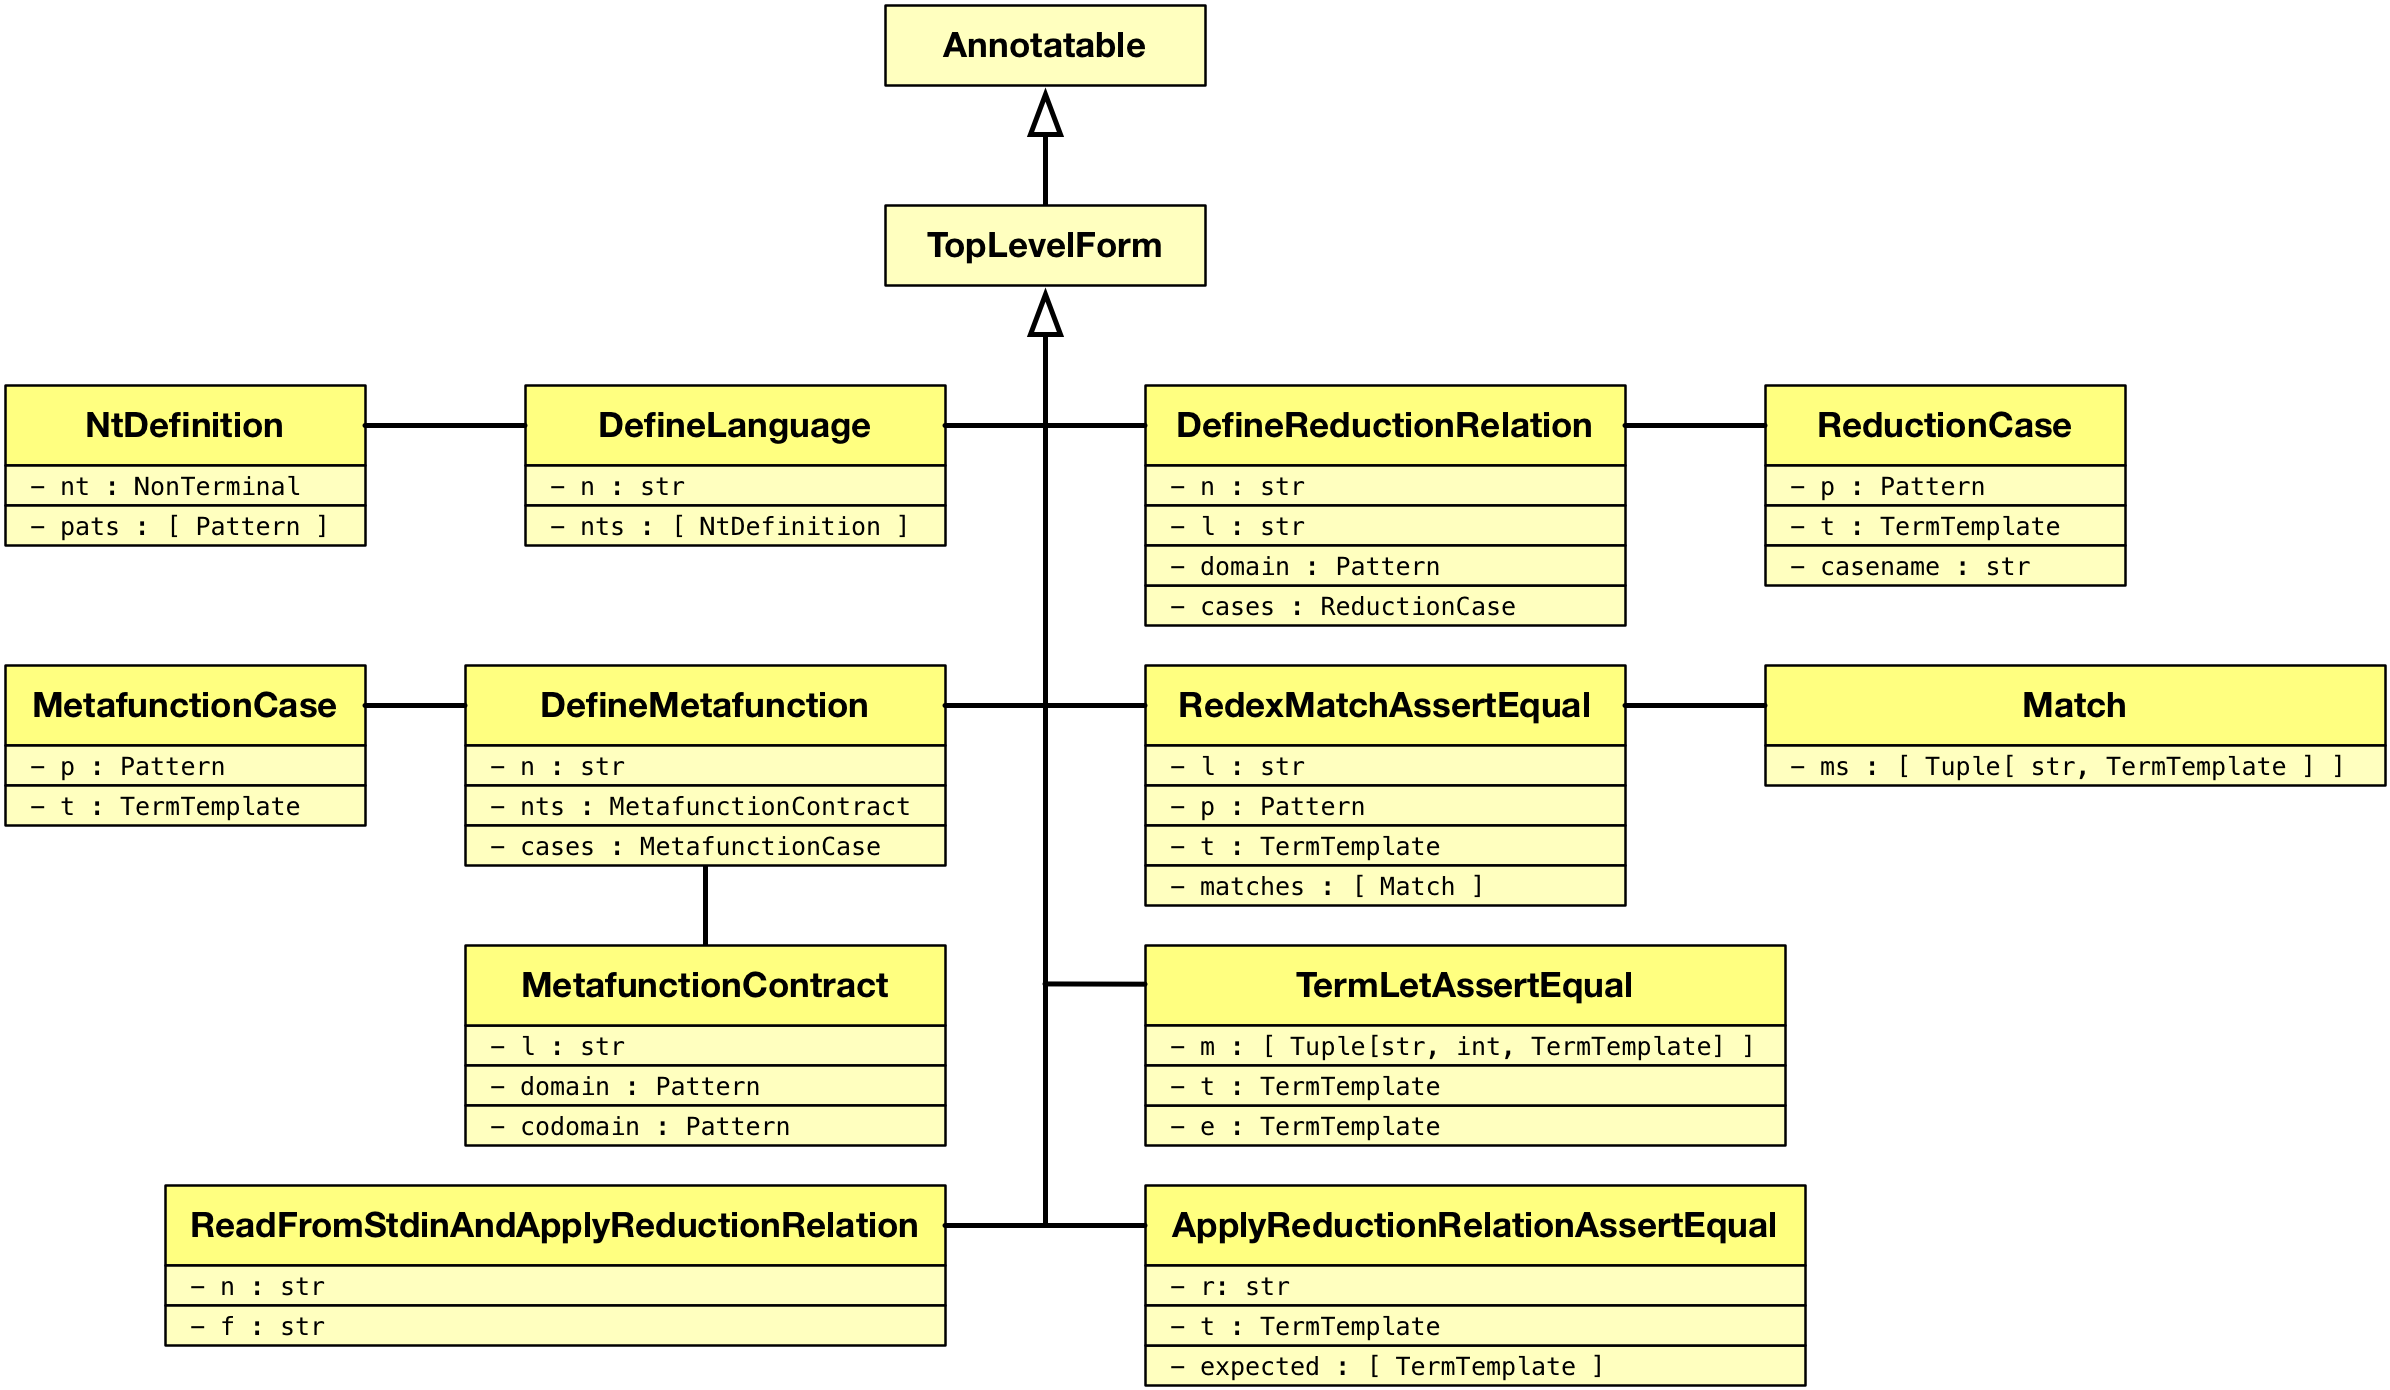
\includegraphics[scale=0.21]{class-diagram-toplevel.png} }
	\caption{Representation of top-level forms.}
\label{class-diagram-toplevel}
\end{figure}

\section{Visitors}
\label{section:visitors}
Since patterns, term-templates, and top-level forms require analysis or transformations applied to them, visitors for each \texttt{TermTemplate}, \texttt{Pattern} and \texttt{TopLevelForm} are provided, as seen in Figure \ref{class-diagram-visitors}.

In other programming languages the \texttt{Visitor} design pattern would require each \newline \texttt{TermTemplate}, \texttt{Pattern} or \texttt{TopLevelForm} class to implement the \texttt{accept} method with \texttt{Visitor} passed as a parameter. However, since Python is a dynamic language, it is possible to invoke methods given their names as strings. The \texttt{\_visit} method does exactly that - it looks up the type-name of a passed element, constructs the string, attempts to retrieve the method, and calls it. For example, given the \texttt{PatternSequence} instance, the resulting method name would be \texttt{\_visitPatternSequence}.

The only method of interest left is \texttt{run}. It is expected to be overridden by each transformation or analysis pass.  Since patterns used in \texttt{define-language} form require different treatment, \texttt{run} implementation may contain iteration logic over \texttt{define-language}, calling \texttt{\_visit} on each pattern.

\section{\texttt{Annotatable} Class}

When applying Transform/Analysis Passes to top-level forms, patterns, and term-templates, additional information needs to be stored pertaining to those elements. One more obvious idea is to store those bits of information in a separate hash-map or dictionary, with \texttt{TermTemplate}, \texttt{Pattern} or \texttt{TopLevelForm} instances acting as keys. However, since a given instance may be completely replaced with something else during transformation, the key of the dictionary has to also be updated, making dictionary management a necessity.

PyPltRedex solves this by storing these bits of information directly into the nodes. \texttt{TermTemplate}, \texttt{Pattern}, and \texttt{TopLevelForm} are subclasses of the \texttt{Annotatable} class. The class diagram can be seen in Figure \ref{class-diagram-visitors}.

Python's dynamicity is leveraged to store arbitrary information in the dictionary with \texttt{str} instances acting as keys. \texttt{addmetadata} adds data to the dictionary, \texttt{getmetadata} retrieves it from the dictionary. \texttt{removemetadata} removes a key-value pair from the dictionary. \texttt{copymetadatafrom} makes a shallow copy of the dictionary of the provided element, if the element is being replaced by something else.

\begin{figure}[ht]
	\centering
	\makebox[\textwidth][c] { 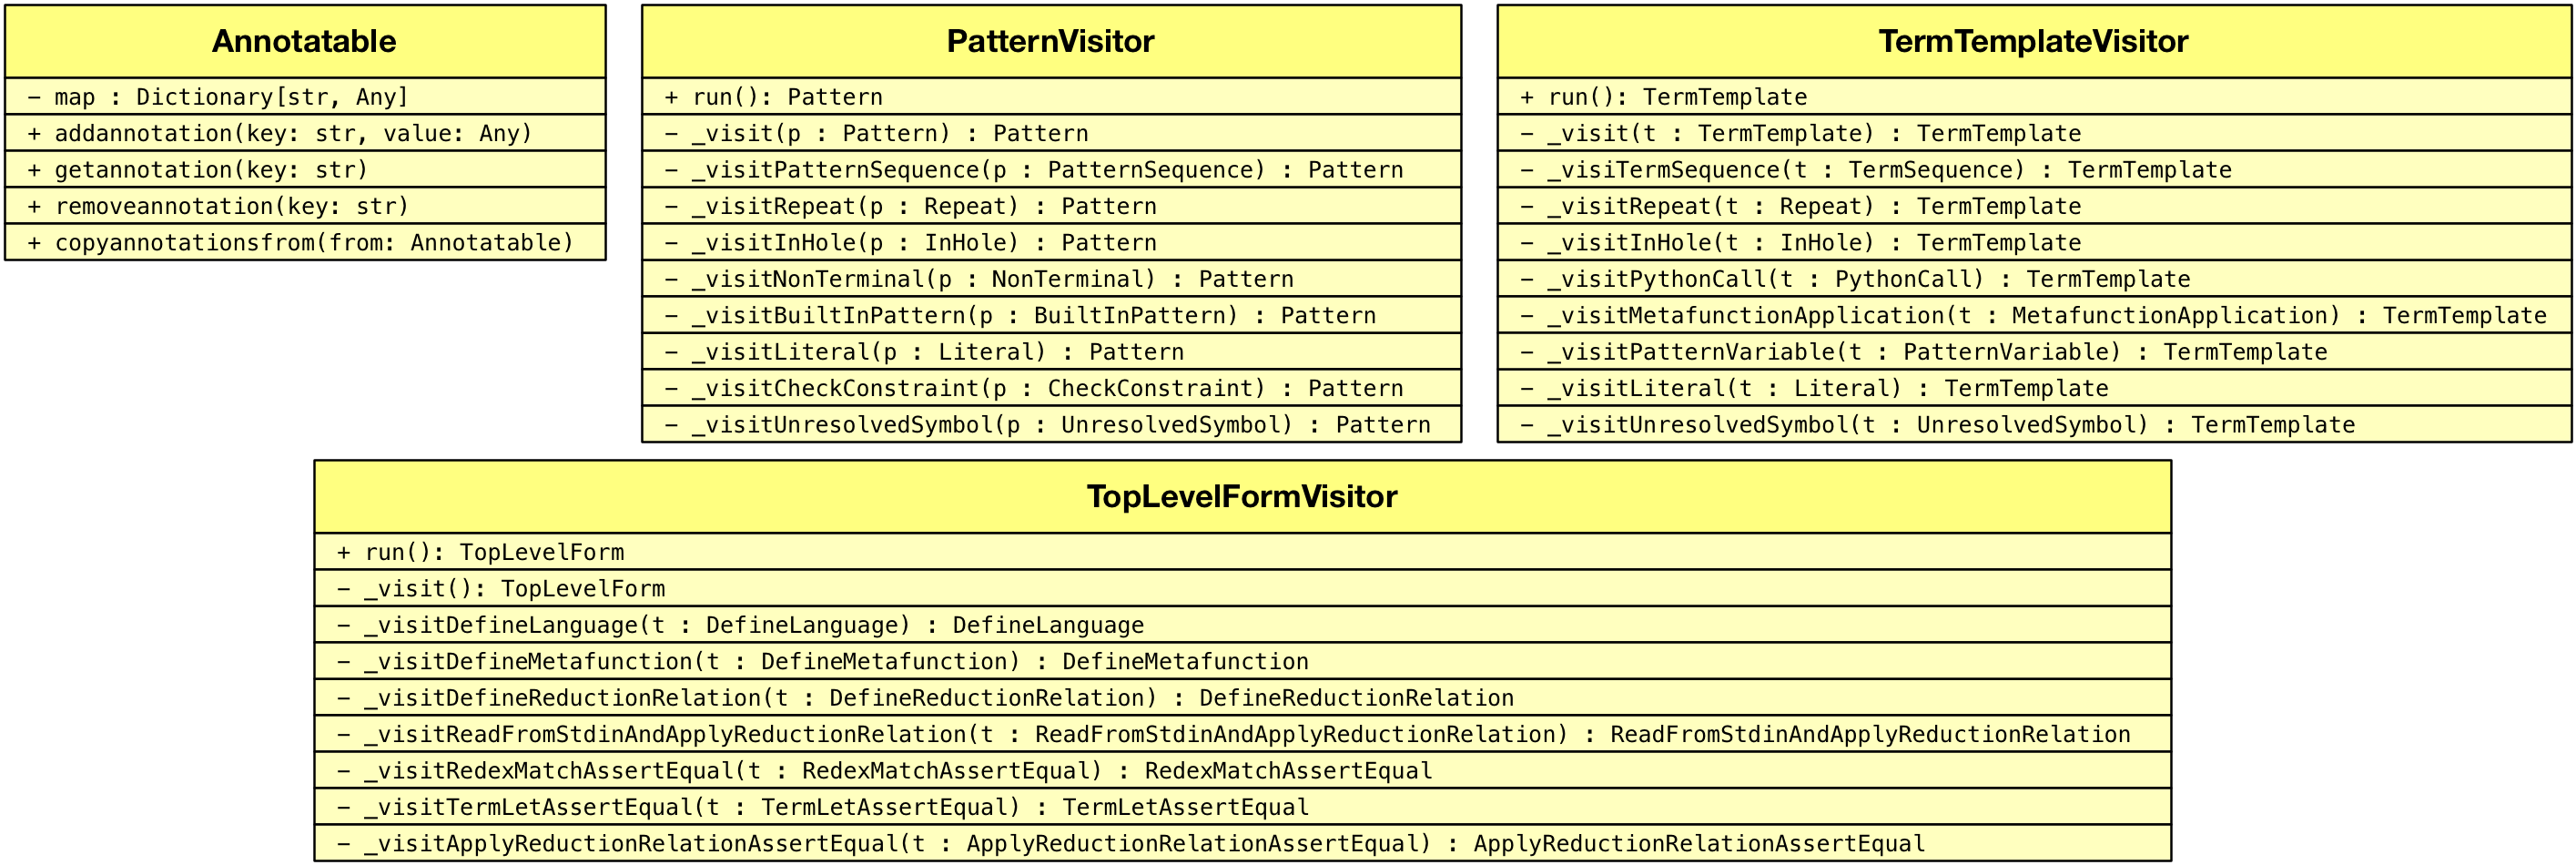
\includegraphics[scale=0.20]{class-diagram-visitors.png} }
	\caption{Representation of visitors and \texttt{Annotatable} class.}
\label{class-diagram-visitors}
\end{figure}

\FloatBarrier


\chapter{Preprocessing Patterns, Term-Templates, and Top-Level Forms}

This section describes Transformation/Analysis Passes that are applied to patterns and \texttt{define-language} forms. Most of these are based on \texttt{Visitor} classes described in Section \ref{section:visitors}.


\section{Pattern: Pattern-Variable Resolution}
\label{section:pv-resolve}

\subsection{Algorithm}

Immediately after parsing the PLTRedex specification, it is unknown whether certain elements of a pattern are built-in patterns, non-terminal symbols or just literals. These elements are represented with \UnresolvedSymbol instances and will have to be resolved in one of the following ways: \BuiltInPatternNoArg, \NonTerminalNoArg, or \LiteralPatternNoArg.

If this transformation is being applied to \texttt{define-language} form, all sub-patterns that resolve to \LiteralPatternNoArg \space need to be stored in set $V$ (initially empty) which is the set of all variables used by the given language. After applying the transformation, \texttt{define-language} $l$ form has to be annotated with $V$ - \MakeAnnotation{$l$}{"ReservedVariables"}{$V$}.

Given \LetDefineLanguage{$l$}, let $\mathit{Nt_{l}}$ be the set of all non-terminal symbols of the language. Given string $\mathit{sym}$, the prefix of $\mathit{sym}$ needs to be extracted. Let $\mathit{prefix_{sym}}$ be a string of characters up to the first occurrence of an underscore character in $\mathit{sym}$. There are several cases to consider.

\begin{itemize}
\item $\mathit{prefix_{sym}}$ does not exist; there are no underscore characters in $\mathit{sym}$. Let $\mathit{prefix_{sym}=sym}$.
\item $\mathit{prefix_{sym}}$ is empty; the first character of $\mathit{sym}$ is underscore. Raise an Exception because PLTRedex doesn't consider such symbols valid.
\item Otherwise, $\mathit{prefix_{sym}}$ is the prefix.
\end{itemize}

The resolution algorithm proceeds in the following manner. The pattern is traversed recursively. When coming across \UnresolvedSymbol \space node, extract $\mathit{prefix_{sym}}$. One of the following cases may happen.

\begin{itemize}
\item Prefix is \texttt{number}, return \BuiltInPattern[Number][$\mathit{sym}$][false].
\item Prefix is \texttt{integer}, return \BuiltInPattern[Integer][$\mathit{sym}$][false].
\item Prefix is \texttt{real}, return \BuiltInPattern[Real][$\mathit{sym}$][false].
\item Prefix is \texttt{natural}, return \BuiltInPattern[Natural][$\mathit{sym}$][false].
\item Prefix is \texttt{string}, return \BuiltInPattern[String][$\mathit{sym}$][false].
\item Prefix is \texttt{boolean}, return \BuiltInPattern[Boolean][$\mathit{sym}$][false].
\item Prefix is \texttt{variable-not-otherwise-mentioned}, \\ return \BuiltInPattern[Variable][$\mathit{sym}$][false]
\item Prefix is \texttt{hole}. Since PLTRedex doesn't allow underscores for \texttt{hole} patterns check if $\mathit{prefix(sym) \neq sym}$ and raise an Exception accordingly. \\ Return \BuiltInPattern[Hole][$\mathit{sym}$][false].
\item $\mathit{prefix_{sym} \in Nt_l}$, return \NonTerminal[$\mathit{prefix_{sym}}$][$\mathit{sym}$][false].
\item Finally, ensure that symbol does not contain underscores. PLTRedex only allows underscores after non-terminal symbols and built-in patterns. Abort compilation process if that is the case. Otherwise, $V=V\cup\{\mathit{sym}\}$ and return \LiteralPattern[Variable][$\mathit{sym}$][false]
\end{itemize}

\subsection{Example}

\begin{figure}[ht]
	\makebox[\textwidth][c] { 
		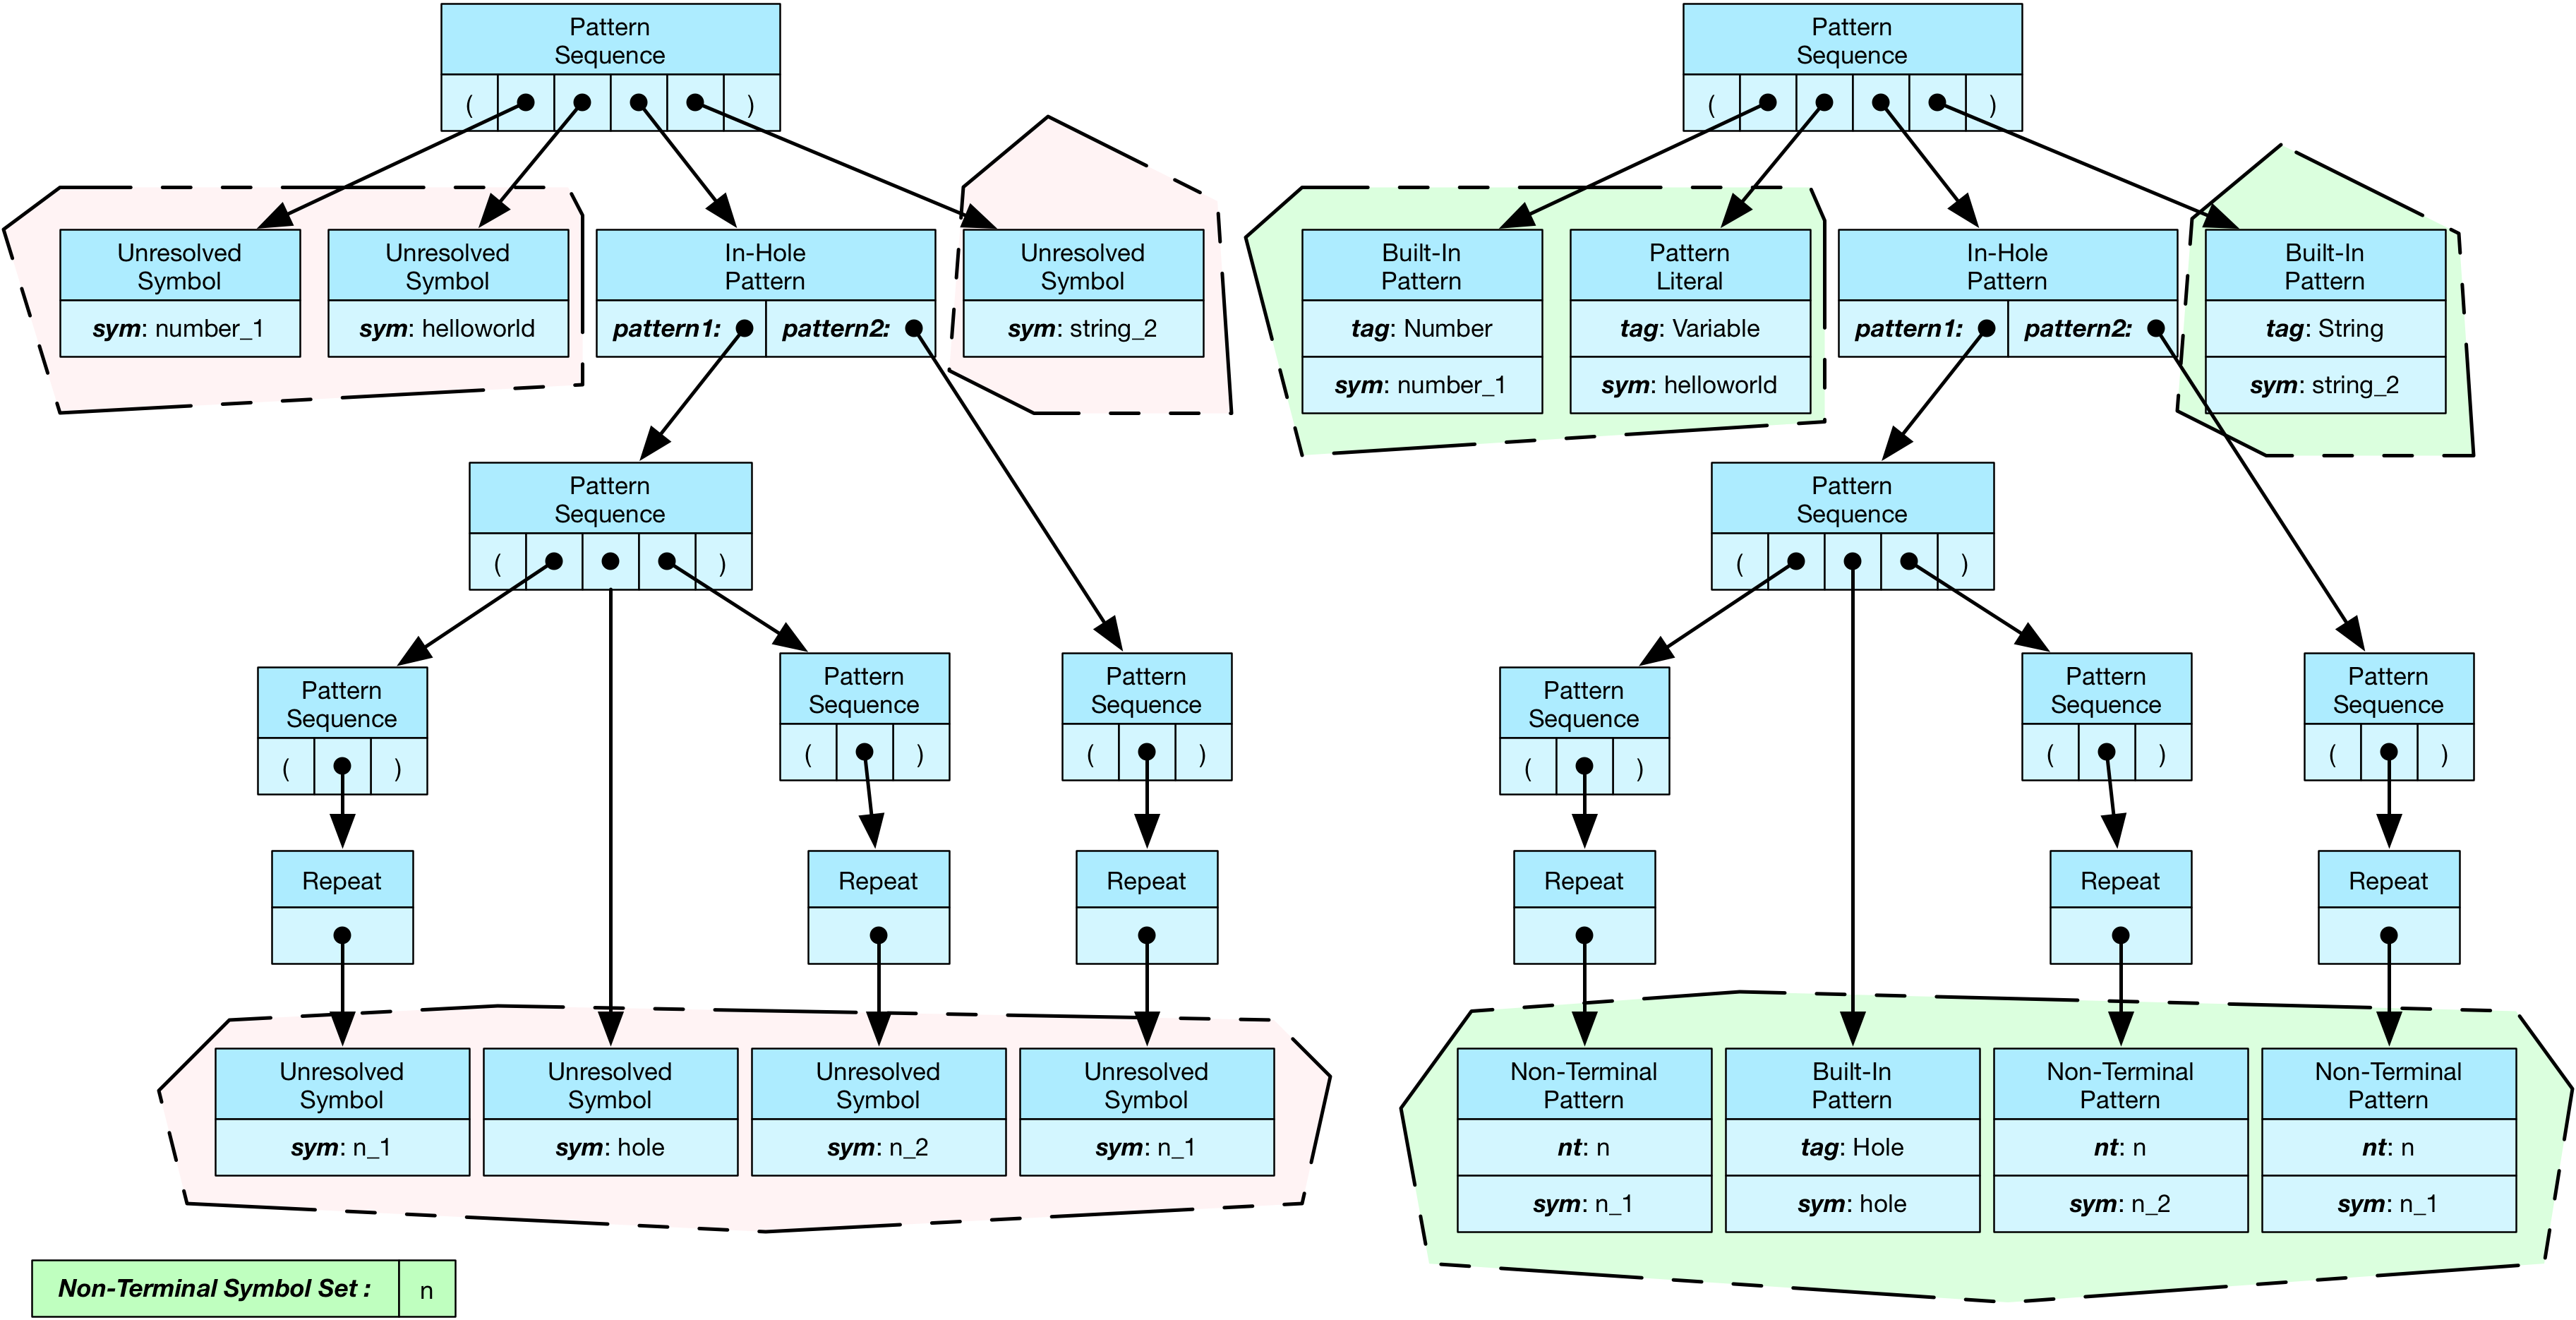
\includegraphics[scale=0.13]{transformation-pattern-resolvesym.png}
	}
\caption{Pattern before and after pattern variable resolution.}
\label{transformation-pattern-resolvesym}
\end{figure}

Figure \ref{transformation-pattern-resolvesym} shows an effect of transformation on pattern \texttt{(number\_1\ helloworld\ (in-hole\ ((n\_1\ ...)\ hole\ (n\_2\ ...))\ (n\_1\ ...))\ string\_2)}. Assume the related \texttt{define-language} has a single non-terminal \texttt{n}. Initially the pattern has six unresolved symbols - \texttt{number\_1}, \texttt{helloworld}, \texttt{n\_1}, \texttt{n\_2}, \texttt{hole} and \texttt{string\_2}. \texttt{number\_1}, \texttt{string\_2}, and \texttt{hole} become \texttt{BuiltInPattern} with appropriate tags,  \texttt{n\_1} and \texttt{n\_2} turn into non-terminals because prefix \texttt{n} is in the set of non-terminal symbols of given \texttt{define-language} and \texttt{helloworld} becomes a \texttt{LiteralPattern} with tag \texttt{Variable}. If this pattern were a part of \texttt{define-language}, \texttt{helloworld} would have been included into set $V$.

\section{DefineLanguage: Identifier Rewriting}
\label{section:id-rewrite}

\subsection{Motivation}

For patterns in the \DefineLanguageNoArg \space constraint checking is not performed. This means that in this context, patterns \texttt{(+ e e)} and \texttt{(+ e\_1 e\_1)} are equivalent. Due to design of \texttt{Match} class described in Section \ref{section:Match}, PyPltRedex needs to modify all such pattern-variables to be unique. Given the pattern-variable $pv$, $\mathit{prefix_{pv}}$ (defined in Section \ref{section:pv-resolve}) is extracted and concatenated with some previously unused integer - $\mathit{freshint()}$.

\subsection{Algorithm}
Given \LetDefineLanguage{$l$}, each pattern $p_i$ in \NtDefinitionN \space is visited recursively.
\begin{itemize}
\item Given \BuiltInPattern, \\ return \BuiltInPattern[$\mathit{tag}$][$\mathit{prefix_{pv}+freshint()}$][false].
\item Given \NonTerminal, \\ return \NonTerminal[$\mathit{nt}$][$\mathit{prefix_{pv}+freshint()}$][false].
\end{itemize}

\subsection{Example}

Figure \ref{id-rewrite-example} shows an example of the transformation on the \DefineLanguage form. Numerical suffixes are added to each occurrence non-terminal \texttt{e}, \texttt{n} and built-in pattern \texttt{number}.

\begin{figure}[h]
	\begin{minipage}{0.5\linewidth}
		\centering
		\begin{minted}[tabsize=2,obeytabs,escapeinside=||,mathescape=true,fontsize=\small]{Racket}
(define-language L
	(e ::= (+ |\colorbox{identbefore}{e} \colorbox{identbefore}{e}|)
	       (* |\colorbox{identbefore}{e} \colorbox{identbefore}{e}|) |\colorbox{identbefore}{n}|)
	(n ::= |\colorbox{identbefore}{number}|))
		\end{minted}
	\end{minipage}
	\begin{minipage}{0.5\linewidth}
		\centering
		\begin{minted}[tabsize=2,obeytabs,escapeinside=||,mathescape=true,fontsize=\small]{Racket}
(define-language L
	(e ::= (+ |\colorbox{identafter}{e\_0} \colorbox{identafter}{e\_1}|)
	       (* |\colorbox{identafter}{e\_2} \colorbox{identafter}{e\_3}|) |\colorbox{identafter}{n\_0}|)
	(n ::= |\colorbox{identafter}{number\_0}|))
		\end{minted}
	\end{minipage}
	\caption{\texttt{define-language} before and afte renaming of identifiers.}
	\label{id-rewrite-example}
\end{figure}

\section{Pattern: Ellipsis Depth Checking}

\subsection{Motivation}

Pattern-variables with the same symbol should be under a consistent number of ellipses. For example, in pattern \texttt{(((n\_1 ...)\ n\_1)\ ...)} the pattern variable \texttt{n\_1} is not under a consistent number of ellipses - one ellipses has an \textit{ellipsis depth} of one, whereas the other is two. Such invalid patterns should be reported during the compilation process.

In addition, after pattern matching, the pattern-variables are plugged into term-templates and the ellipsis depth of each pattern-variable is needed to ensure that a given term-template is well-formed.

\subsection{Algorithm}

During pattern traversal, the following need to be maintained:

\begin{enumerate}
\item
Let $n$ be \textbf{number of ellipses} on the path from the root of the pattern to some child sub-pattern. $n$ is modified accordingly when visiting patterns of kind \RepeatNoArg.

\item Association between pattern-variable $pv$ and its ellipsis depth $d$. Let $E=\emptyset$ containing pairs $(pv, d)$.
\end{enumerate}

Given some pattern $p$, \Visit{$p$}. The following kinds of $p$ are of interest.
\begin{itemize}
\item $p=$\space \PatternRepeat. Let $n=n+1$, \Visit{$p_r$}, and then let $n=n-1$.
\item $p=$\space \BuiltInPattern. Check if there exists a pair $(pv, d) \in E$. If it does not, $E = E \cup \{ (pv, d) \}$. Otherwise, if $n \neq d$, then $pv$ has inconsistent ellipsis depth and an Exception is raised.
\item $p=$\space \NonTerminal \space is handled in the same way as \BuiltInPatternNoArg.
\end{itemize}

Finally, the pattern $p$ has to be annotated with $E$ - \MakeAnnotation{$p$}{"EllipsisDepths"}{$E$}.

\section{DefineLanguage: Non-Terminal Cycle Checking}

\subsection{Motivation}
PltRedex doesn't allow language definitions such as the one in Figure \ref{dl-ntcyclegraph}.

\begin{figure}[H]

	\centering
\begin{minipage}{0.45\linewidth}
\begin{minted}[tabsize=1,obeytabs,escapeinside=||,mathescape=true,linenos,fontsize=\small]{racket}
(define-language L
	(e ::= (e e) n)
	(n ::= (n n) number p)
	(p ::= (p p) real e))
	(s ::= string)
\end{minted}
\end{minipage}
\begin{minipage}{0.45\linewidth}
	\centering
	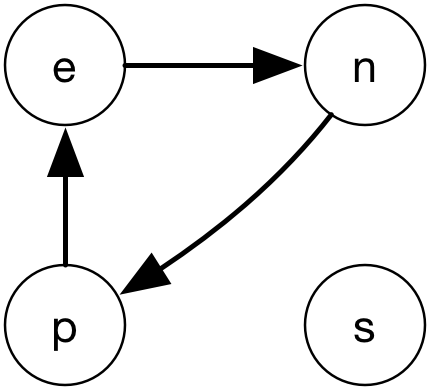
\includegraphics[scale=0.18]{transformation-pattern-ntgraph.png}
\end{minipage}
	\caption{\texttt{define-language} and its non-terminal graph}
	\label{dl-ntcyclegraph}
\end{figure}

The problem with the language above (aside from it being completely useless) is a cycle of non-terminals $n \rightarrow p \rightarrow e$. When testing if some term is a non-terminal, a term is matched against every pattern in a non-terminal definition. For example, given term \texttt{String("hello world")}, it is matched against non-terminal \texttt{e}. Since  the term doesn't match the pattern \texttt{(e e)}, non-terminal \texttt{n} is then matched. Since the term doesn't match any patterns here either, non-terminal \texttt{p} is then matched. Similarly, the term doesn't match any patterns here either, \texttt{e} is then matched, but that's where the matching has started and thus \textit{infinite recursion} becomes an issue. Languages need to be analyzed for presence of non-terminal cycles.

\subsection{Algorithm}
To detect such cycles, \DefineLanguageNoArg \space needs to be interpreted as a directed graph and some cycle-detecting algorithm must be used. The graph is constructed in the following manner.

\begin{enumerate}
\item
For each \NtDefinitionN[n], create a vertex labeled $n$.
\item
For $p_1, ..., p_n$, if $p_i$ is \NonTerminal[m][m\_?], create the edge $n\rightarrow m$.
\end{enumerate}


To detect cycles, depth-first-search is employed. Vertices in the graph can be assigned one of three colors:

\begin{itemize}
\item

\textbf{White} - meaning the vertex hasn't been visited before. All vertices are initially assigned this color.

\item
\textbf{Gray} - meaning successors of the vertex $v$ are still being visited. When $v$ is visited for the first time, $color(v)$ becomes \textbf{Gray}.
\item
\textbf{Black} - meaning all successors of the vertex $v$ have been explored.
\end{itemize}

A path of vertices visited during depth-first traversal is maintained.  Let $V$ be a set of vertices whose \DFSColor{$v$}{Black}, initially empty; let $U$ be a set of vertices whose \DFSColor{$v$}{White}, initially containing all vertices of the graph.

The algorithm proceeds in the following way:

\begin{enumerate}
\item Pick random vertex $u \in U$.
\item If \DFSColor{$u$}{White}, set color to \textbf{Gray} and add $u$ to the path.
\item If \DFSColor{$u$}{Gray}, report the cycle (using vertices on the path) and abort compilation.
\item Visit each successor vertex $u^{\prime}$ of $u$ recursively.
\item Set color of $u$ to \textbf{Black} and remove it from the path. $V = V \cup \{u\}$.
\item If there are no more vertices left to visit, let $U = U-V$ and go to step 1.
\end{enumerate}

It should be noted that the algorithm described does not report all the cycles in the graph but the first one it manages to find. One improvement could be finding all cycles in the graph.

%\section{Hole Reachability}

The pattern \InHolePattern requires $p_1$ to match exactly one \lstinline{hole} term. The main problem is counting a number of holes matched by non-terminal symbols of the language. Consider the language \lstinline{MatchesManyHoles} listed below.

\begin{lstlisting}
(define-language MatchesManyHoles
	(n ::= number)
	(P ::= E (n ... E ...))
	(E ::= (+ E P) (+ n E) hole))
\end{lstlisting}

To compute value for  the non-terminal \lstinline{E}, an analysis of pattern \lstinline{(+ E P)} is required but the value of \lstinline{E} is not yet known. Moreover, computing a single value that represents number of holes is insufficient; pattern lstinline{(E ...)} may match zero or many holes. Thus, a \textbf{minimum} and \textbf{maximum} number of holes matched by some pattern must be computed.

\subsection{Graph Modeling}

Graph consists of two parts - \textbf{outer-nodes} and \textbf{inner-nodes}.

Outer-nodes are a stand-in for the pattern and come in four different varieties:

\begin{itemize}
\item \lstinline{Sequence} representing pattern-sequences.
\item \lstinline{Repeat} representing ellipses.
\item \lstinline{LeafHole} representing the pattern \lstinline{hole}.
\item \lstinline{LeafNotHole} representing any other pattern except \InHolePattern
\end{itemize}

Inner-nodes are stored in \lstinline{Sequence} and \lstinline{Repeat} outer-nodes and act as non-terminal references. Each inner-node has a set of outer-node successors pointing to a set of expressions that the non-terminal matches.

Graph for language defined above can be seen in the following figure:
TODO

\subsection{Graph Construction}

Constructing the graph involves two stages:
\begin{enumerate}
\item
Creation of outer nodes for each top-level pattern such as `(+ E P)` or `hole`.
\item
Creation of inner nodes and edges from inner to outer nodes. If the outer node is a `Sequence` and it contains other sequences or ellipses, additional creation of outer-nodes will be required.
\end{enumerate}


\subsection{Creation of Outer Nodes}

A mapping of `M` has to be maintained between patterns in non-terminal definition. For each non-terminal definition `N` let `E\_N = \{\}` be a set storing top-level non-terminal references. For example, in the language described above for non-terminal definition `P` the only such reference is `E`.

Each non-terminal definition `N` is visited and we may come across the following patterns.
\begin{itemize}

\item
\BuiltInPattern. If kind is `Hole` then `n = LeafHole` node is created.  Otherwise, `n = LeafNotHole` node is created. Thus, `M = M union {(p, n)}`.
\item
\Nt. This means that `N` is also `nt` and thus all expressions in non-terminal definition of `nt` should also be reachable from any inner-node that reaches expressions in `N`. Thus, `E\_N = E\_N union {nt}`.
\item
\InHolePattern. Raise compilation error and quit. This, however, is not actual behavior of the PltRedex. (TODO explain why we handle it differently?)
* `p = PatternSequence(pattern ...)`. If length of `p` is zero, then `n = LeafNotHole`, otherwise `n = Sequence`. Thus, `M = M union {(p, n)}`.
\end{itemize}

Note that creating multiple `LeafHole` or `LeafNotHole` nodes is not necessary and existing nodes of these kinds can be reused. This means that the graph may have at most two leaf nodes.


\subsection{Creation of Inner Nodes and Edges}

The only top-level pattern kind that may contain inner nodes at this point is `Sequence` and thus they need to be visited. One thing that needs to be maintained is the stack `S` of outer-nodes where inner-nodes are to be stored.

For each non-terminal definition `N` and each pattern $p_i$, if $p_i$ is `PatSequence`, retrieve `M[$p_i$]` from the mapping and place on top of the stack S. For each subpattern $q_i$ in $p_i$, visit $q_i$.

\begin{itemize}
\item
\PatternSequence. Create outer-node `Sequence` `s` for `p`; create inner node `i`; add edge `i->s`. Retrieve parent outer-node `O` and add node `i` to it. Append `s` to the stack `S`. For each child pattern $c_i$ of `p`, recursively visit each $c_i$. Pop topmost element off the stack `S`.

\item
* \Repeat. Create outer-node `Repeat` `r` for `p`, create inner node `i`, add edge `i->r`. Retrieve parent outer-node `O` and add node `i` to it. Append `r` to the stack `S`. Visit child pattern `c` of `p`. Pop topmost element off the stack `S`.

\item
\InHolePattern Raise compilation error and quit.

\item
\BuiltInPattern. Create inner node `i`. If kind is Hole then let s = LeafHole, otherwise s = LeafNotHole. Create edge `i->s`.  Retreieve parent outer-node `O` from the top of the stack and add node `i` to it.

\item
\Nt Create inner node `i`. For each pattern in non-terminal definition of `nt`, retrieve outer-node `o` from the mapping `M` and create edge `i->o`. Do the same for each non-terminal in the set `E\_nt`. Retrieve outer-node `O` from the stack and append `i` to it.

\end{itemize}

\subsection{Minimal/Maximal Value Representation and Arithmetic}

Minimum / maximum number of holes can be one of the following: `Zero`, `One`, `Many` (i.e. >= 2) and `Uninitialized` indicating said value should not be used for computation just yet.

Furthermore, three operators need to be defined - `+`, `min`, `max`. Assume Zero = 0, One = 1, Many = 2 and Uninitialized = 3

Addition operation.

\begin{align}
	a + b =
	\begin{cases}
		3 \text{ if } a = 3 \text{ and } b = 3 \\
		a \text{ if } b = 3 \\
		b \text{ if } a = 3 \\
		min(a + b, 2)
	\end{cases}
\end{align}

Min operation:

\begin{align}
	min(a,b) =
	\begin{cases}
		3 \text{ if } a = 3 \text{ and } b = 3 \\
		a \text{ if } b = 3 \\
		b \text{ if } a = 3 \\
		min(a, b)
	\end{cases}
\end{align}

Max operation:
\begin{align}
	max(a, b) =
	\begin{cases}
		3 \text{ if } a = 3 \text{ and } b = 3 \\
		a \text{ if } b = 3 \\
		b \text{ if } a = 3 \\
		max(a, b)
	\end{cases}
\end{align}


\subsection{Computation of Values}
Min/max values are computed both for inner-nodes and outer-nodes. First, they have to be initialized.

\begin{itemize}
\item
Inner nodes are initialized with (Uninitialized, Uninitialized)
\item
`Sequence` and `Repeat` outer nodes are initialized with (Uninitialized, Uninitialized)
\item
`LeafHole` outer node is initialized with (One, One)
\item
`LeafNotHole` outer node is initialized with (One, One)
\end{itemize}


Given initial values $min_inner$, $max_inner$ of some inner-node  and new values $v_1$, $v_2$, $min_inner = min(min_inner, v1)$, $max_inner = max(max_inner, v2)$.


Given outer-node `o`, there are a few cases to consider.

\begin{itemize}
\item
`LeafHole` and `LeafNotHole` - its min/max values are never updated.
\item
* `Sequence` - $min_o = \sum_{i in inner(o)} min_i$ and $max_o = \sum_{i in inner(o)} max_i$. Summation is described above.
\item
* `Repeat` - $min_o = Zero$, $max_o = Many if max_inner = One or max_inner = Many else Zero$.
\end{itemize}

\subsection{Hole Reachability Algorithm}

Before initiating graph traversal, verify if `LeafHole` node is actually in `V`. If there is no such node, that means the source pattern does not match any `hole` and thus each non-terminal should be annotated with `Zero,Zero` number of holes.

Otherwise, the graph is traversed in reverse direction starting from nodes `LeafHole` and `LeafNotHole` using breadth-first strategy. Maintain queue Q that initially stores all `LeafHole` and `LeafNotHole` nodes.

The algorithm is as follows:
\begin{enumerate}
\item
Remove outer node `o` from the queue `Q`.
\item
* For each inner-node `i` such that `i->o`:
	\begin{enumerate}
	\item
	if `parent(i) = o` then $update(i, o_min, o_max)$ and `update(o)`. This means that if the inner node contains an edge to the outer-node `o` `i` is a child of, thus can be considered a "self-loop". The reason for doing this will be discussed later. (TODO is this actually needed aside from really degenerate patterns?)
	\end{enumerate}

\item
For each inner-node `i` such that `i->o`:
	\begin{enumerate}
	\item
	if `parent(i) != o`, $update(i, o_min, o_max)$ and update(o). If values of $o_min, o_max$ are different from ones before update operation, add `o` to the queue `Q`.
	\end{enumerate}

\item
* Repeat until queue `Q` is empty.

\end{enumerate}


\subsection{Computing Min/max values for non-terminal definition}

Given non-terminal definition `nt` and set of patterns `P` it matches, $min_nt = max_nt = Uninitialized$. Then, $min_nt = \min_{i in P} min_i$ and $max_nt = \max_{i in P} max_i$.Note that some parrern `i` in `P` may be Nt, in which case $min_i$ and $max_i$ for non-terminal definition `i` first. By ensuring that language contains no non-terminal cycles, such recursive procedure s guaranteed to terminate.

After completing all computations, each non-terminal definition `nt` is annotated with corresponding $min_nt, max_nt$.


\subsection{Edge cases}.

This algorithm doesn't do one very specific thing - infinite terms and presence of `hole`. Consider the language below

\begin{lstlisting}
(define-lagnuge Infinite
     (P ::= (E))
     (E ::= P hole))
\end{lstlisting}

\subsection{Example}
TODO

%\section{Pattern: \lstinline{in-hole} Pattern Checker}

Having computed `min/max` numbers for each non-terminal in the language, now the question is whether `pattern1` in pattern \InHolePattern actually matches exactly one hole. Doing so involves two stages:

\begin{enumerate}
\item
Locating \InHolePattern in the top-level pattern.
\item
Checking if $p_1$ matches exactly one hole. Since $pattern1$ doesn't necessarily have to be a non-terminal, extra work will be required.
\end{enumerate}

\subsection{Checking pattern for number of holes}

Assuming \InHolePattern pattern has already been found, $p_1$ has to be visited recursively. One of the following nodes may be visited.

\begin{itemize}
\item
\BuiltInPattern - if $t=$hole then $min_p = One, max_p = One$, otherwise $min_p = Zero, max_p=Zero$.

\item
\Nt. Read appropriate annotation from non-terminal definition in `define-language` and return values.

\item

\LiteralPattern min\_p = Zero, max\_p = Zero.

\item
\InHolePattern. Return $min_p = Zero, max_p = Zero$, this seems to be default PltRedex behaviour.

\item
\Repeat. Recursively visit the $p$ obtaining $min_p2$, $max_p2$. The logic for Repeat is identical to the one used in **Hole Reachability**; that is:
	\begin{itemize}
	\item
	$min_n = Zero$
	\item
	$max_p = Many if max_p2 = One or max_p2 = Many$
	\item
	$max_p = Zero$ otherwise
	\end{itemize}

\item
* \PatternSequence. Initially, $min_p$, $max_p = Unitialized$. Then, $min_p = \sum_{p_i in p} minp_i$. To obtain $minp_i$, $p_i$ has to be recursively visited.
\end{itemize}

\subsection{Example}
TODO

\section{Pattern: Constraint Check Insertion}
\label{section:constraint-check}
\subsection{Motivation}
As mentioned before, PLTRedex supports a few different forms of constraint checking; however, for the initial PyPltRedex implementation only the "equality of terms" constraint check is supported. For example, in the pattern \texttt{(number\_1 number\_1)} both terms bound to \texttt{number\_1} must be the same, meaning the term \texttt{(1 1)} does match the pattern but \texttt{(1 2)} does not.

However, since the current design of the \texttt{Match} class, explained in Section \ref{section:Match}, does not allow assigning multiple terms to the same pattern-variable, certain pattern-variables have to be renamed. Given $n$ occurrences of a pattern-variable, $n-1$ occurrences are to be renamed. After completion of pattern matching these $n-1$ pattern-variables must be removed from all returned \texttt{Match} instances.

Finally, actual equality checks have to be inserted. There are two obvious strategies that could be employed:

\begin{itemize}
\item Compare required pattern-variables \textit{after} matching a term against a pattern. The disadvantage of this strategy is that the pattern has to be matched entirely despite the fact that failure may happen very early in the matching process, thus resulting in useless work.

\item Compare required pattern-variables at the \textit{earliest} time possible, as pattern-variables become available. This is the strategy that PyPltRedex uses.
\end{itemize}

\subsection{Pattern-Variable Renaming}
Pattern variable $pv$ is renamed in the following manner: $\mathit{pv + \# + freshint()}$, $\mathit{freshint()}$ if $\mathit{freshint() > 0}$ otherwise $pv$. $\mathit{freshint}$ operation was defined previously in Section \ref{section:id-rewrite}. For example, assuming $\mathit{freshint()=0}$, renaming \texttt{m} results in \texttt{m}. Successive application of the renaming operation results in \texttt{$m\#1$}.

\subsection{Algorithm}
Since the algorithm is based on renaming (or modification) of pattern-variables, let $v^{\prime}$ be a new pattern-variable after modifying $v$. The pairs $(pv, pv^{\prime})$ need to be maintained in order to decide where to insert equality checks. Let $M$ be a set containing such pairs. Furthermore, to remove renamed pattern-variables after matching, the set $R$ containing such pattern-variables has to be maintained.

Given some pattern $p$, \Visit{$p$}. The following kinds of $p$ are of interest.
\begin{itemize}
\item $p=$\space \BuiltInPattern. Let $pv^{\prime}$ be a renamed variable and let $M=\{(pv, pv^{\prime})\}$. If $pv \neq pv^{\prime}$, $R=R \cup \{pv^{\prime}\}$. Return \BuiltInPattern[$tag$][$pv^{\prime}$][false] and $M$.
\item $p=$\space \NonTerminal. Let $pv^{\prime}$ be a renamed variable and let $M=\{(pv, pv^{\prime})\}$. If $pv \neq pv^{\prime}$, $R=R \cup \{pv^{\prime}\}$. Return \NonTerminal[$nt$][$pv^{\prime}$][false] and $M$.
\item $p=$\space \LiteralPattern \space contains no pattern-variables and thus $p$ and $\emptyset$ are returned.
\item $p=$\space \PatternRepeat. Let $p_r^{\prime}, M=$\space\Visit{$p_r$}. Return \PatternRepeat[$p_r^{\prime}$], $M$.
\item
$p=$\space \PatternSequence. If the sequence contains no child patterns, return $p$, $\emptyset$. Define \texttt{merge} operation that, given two sets $M_i, M_j$ returns two sets $M_k$ and $M_r$; this operation will be discussed below.
Let $p^{\prime}$ be the pattern sequence that replaces $p$.
Let $p_1^{\prime}, M_1$=\Visit{$p_1$}. Insert $p_1^{\prime}$ into $p^{\prime}$. For $p_i \in p_2, ..., p_n$, let $p_i^{\prime}, M_i$=\Visit{$p_i$}.
	\begin{enumerate}
	\item
	Insert $p_i^{\prime}$ into $p^{\prime}$.
	\item
	Let $M_1$, $M_r$ = \texttt{merge}($M_1$, $M_i$). For each pair of pattern-variables $(pv_a, pv_b) \in M_r$, insert \PatternCheckConstraint[$pv_a$][$pv_b$][false] into $p^{\prime}$.
	\end{enumerate}
Finally, return $p^{\prime}, M_1$.

\item
$p=$\space \PatternInHole.\\ Let $p_1^{\prime}, M_1$= \Visit{$p_1$} and $p_2^{\prime}, M_2$= \Visit{$p_2$}. Let $M, M_r$=\texttt{merge}($M_1$, $M_2$). For each pair of pattern-variables $(pv_a, pv_b) \in M_r$, let $c_i$=\PatternCheckConstraint[$pv_a$][$pv_b$][false]. Return \PatternInHole[$p_1^{\prime}$][$p_2^{\prime}$][$c_1$][$c_n$][false], $M$.
\end{itemize}

Finally, make an annotation \MakeAnnotation{$p$}{"PatConstraintCheckRemoveVars"}{$R$}.

\subsection{\texttt{merge} Operation}
Before proceeding with pattern traversal, \texttt{merge} operation needs to be defined. Given two sets $M_1$ and $M_2$ it produces two sets $M$ and $M_r$. Those sets are constructed in the following manner:

\begin{enumerate}
\item Let $M=\emptyset$ and $M_r=\emptyset$.
\item For each $(pv, pv^{\prime}) \in M_1$, find a pair $(pv, pv^{\prime\prime}) \in M_2$.
\begin{enumerate}
\item If such pair exists, then $M_r=M_r \cup \{(pv^{\prime},  pv^{\prime\prime})\}$ and $M=M \cup \{(pv,  pv^{\prime\prime})\}$.
\item Otherwise, $M=M \cup \{(pv,  pv^{\prime})\}$
\item For any other $(pv, pv^{\prime\prime}) \in M_2$ s.t.  $(pv, pv^{\prime}) \notin M_1$, $M=M \cup \{(pv,  pv^{\prime\prime})\}$
\end{enumerate}
\end{enumerate}

\subsection{Example}

\begin{figure}[htp]
	\centering
	\makebox[\textwidth][c] { 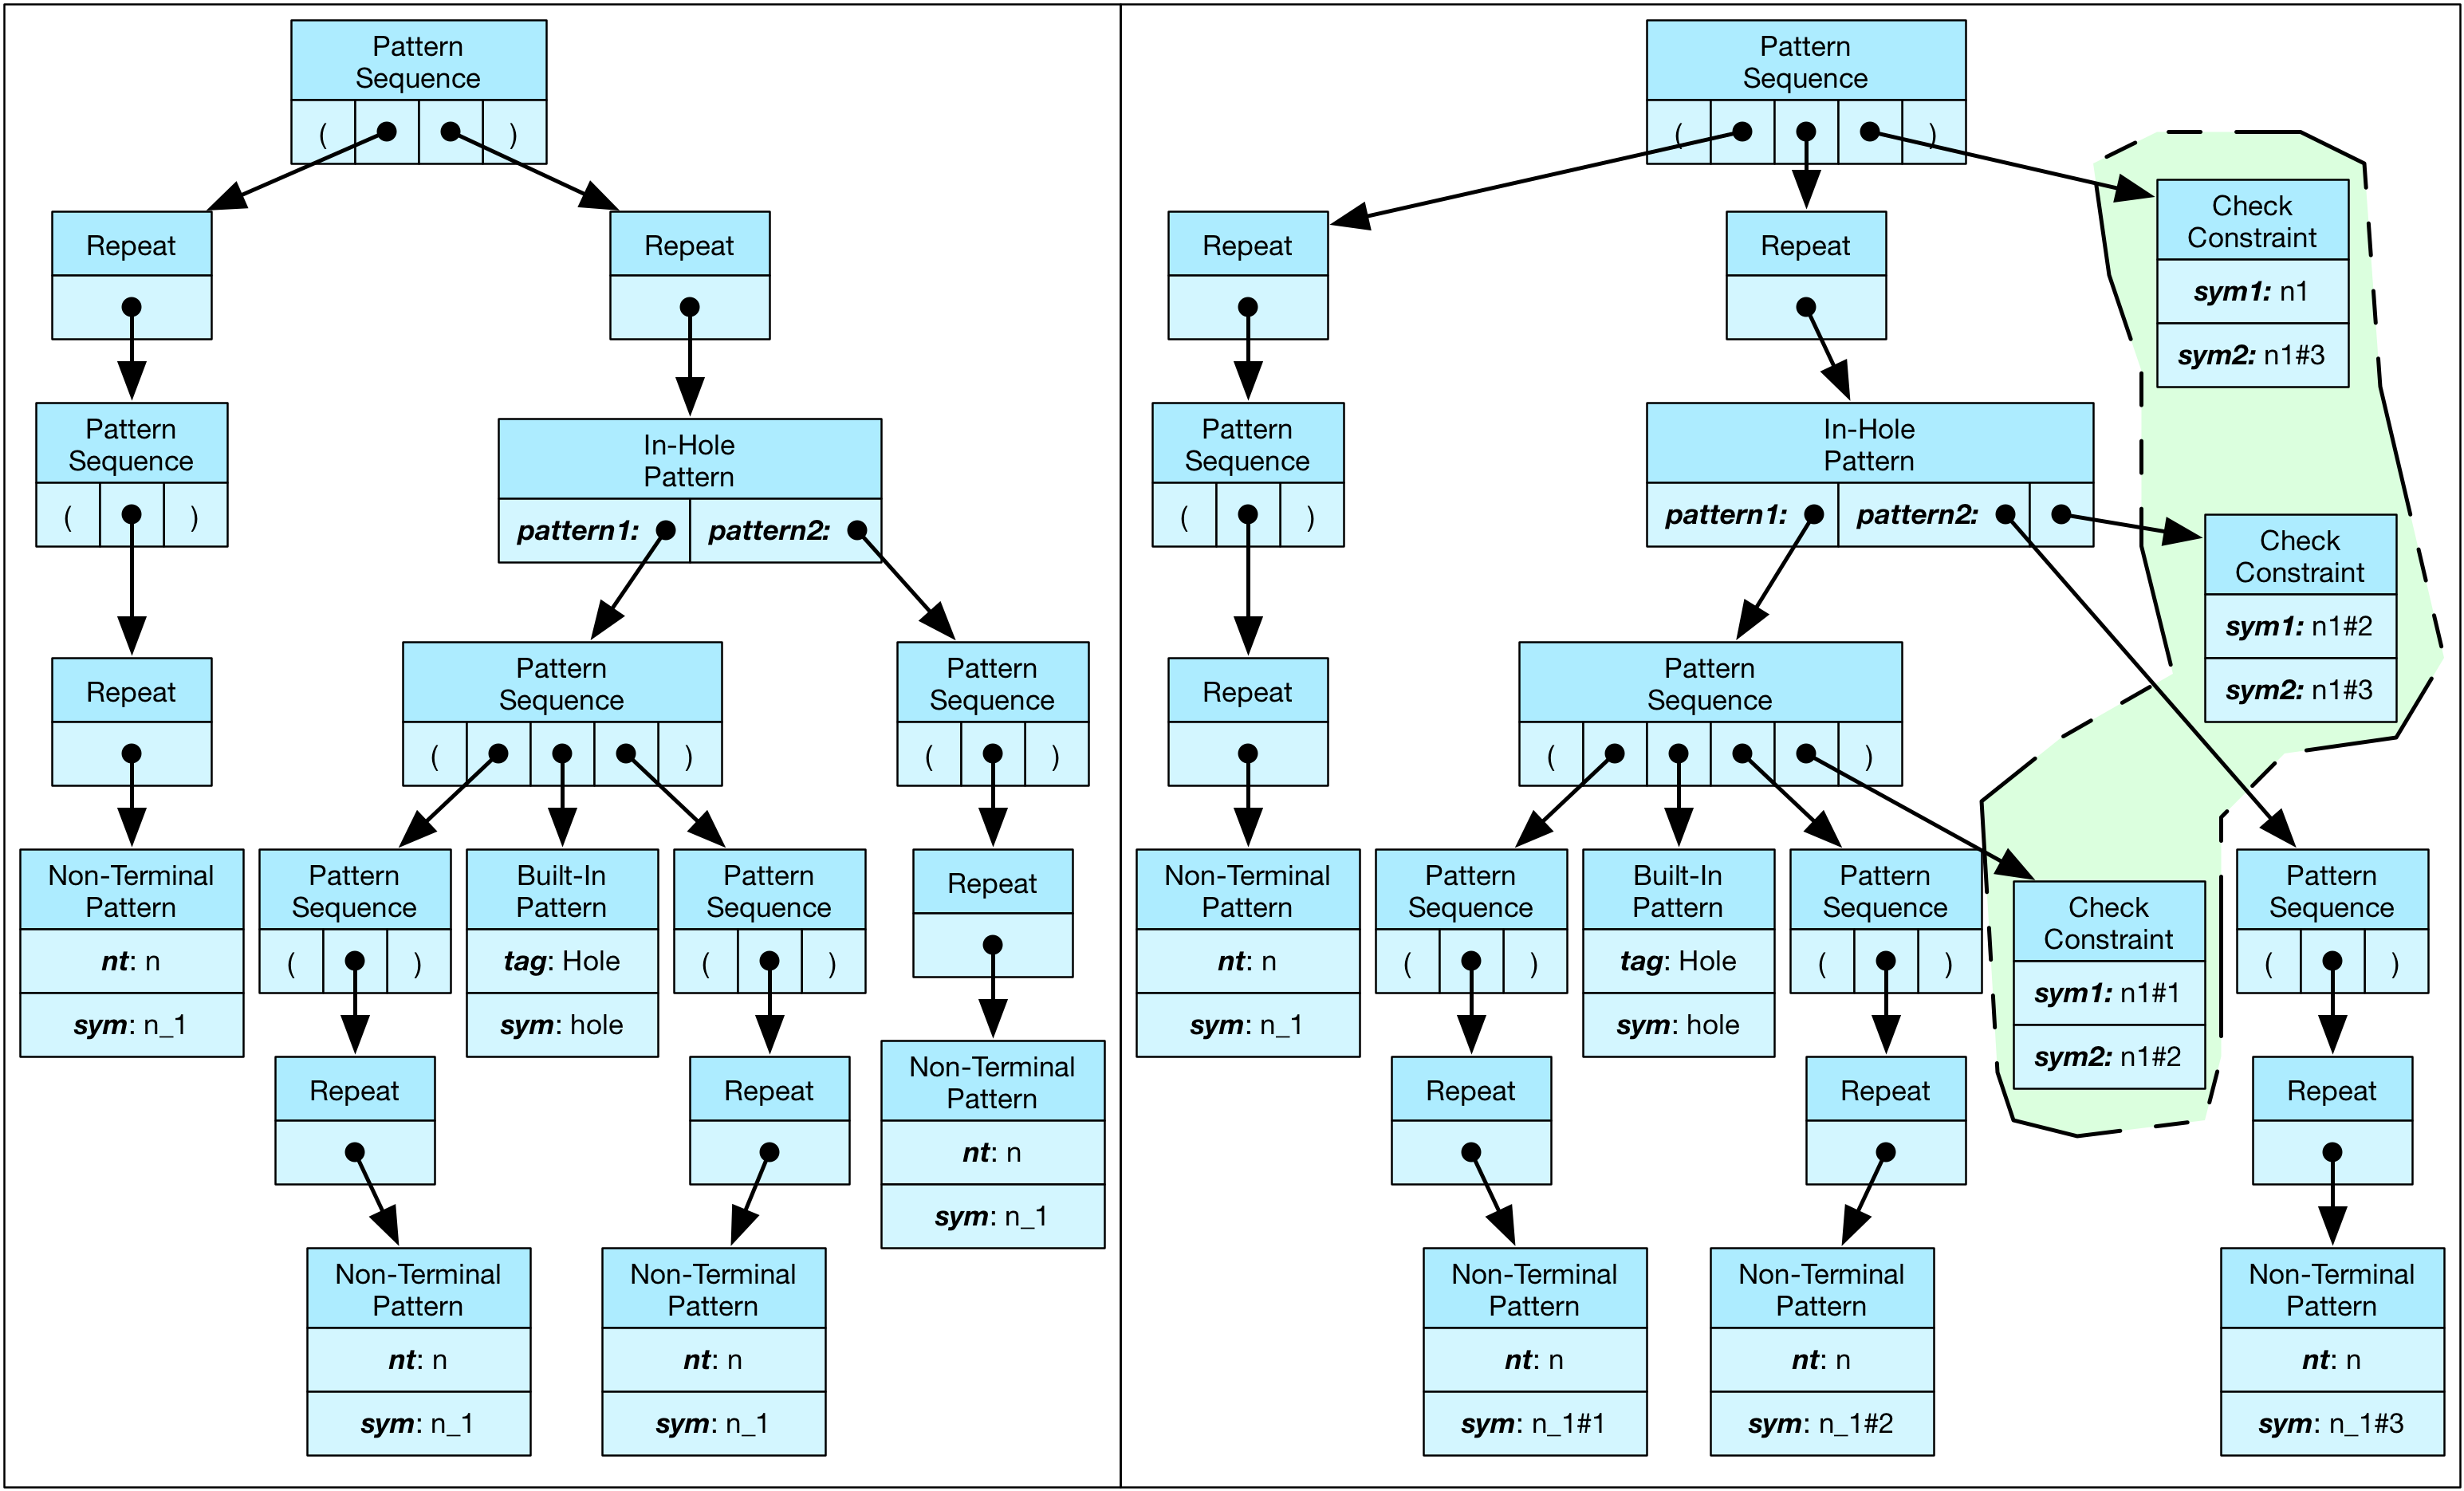
\includegraphics[scale=0.135]{transformation-pattern-constraintcheck.png} }
\caption{Applying transformation to pattern \texttt{((n\_1\ ...)\ ...\ (in-hole\ ((n\_1\ ...)\ hole\ (n\_1\ ...))\ (n\_1\ ...))\ ...)}, before and after.}
\label{transformation-pattern-constraintcheck}
\end{figure}

Figure \ref{transformation-pattern-constraintcheck} shows an effect of described transformation on the pattern \texttt{((n\_1\ ...)\ ...\ (in-hole\ ((n\_1\ ...)\ hole\ (n\_1\ ...))\ (n\_1\ ...))\ ...)}. Notice that all occurrences of \texttt{n\_1} have an ellipsis depth of two. The first occurrence of \texttt{n\_1} goes unmodified. Then, when processing the first pattern inside the \texttt{in-hole} pattern, there are two occurrences of \texttt{n\_1}. The first occurrence is renamed to \texttt{n\_1\#1}, the second to \texttt{n\_1\#2}, and \texttt{CheckConstraint(n\_1\#1, n\_1\#2)} is appended to the \texttt{PatternSequence}. The final occurrence of \texttt{n\_1} is seen in the second pattern of \texttt{in-hole} and is renamed to \texttt{n\_1\#3}. \texttt{CheckConstraint(n\_1\#2, n\_1\#3)} is then added to the \texttt{in-hole}. Finally after exiting \texttt{in-hole}, \texttt{CheckConstraint(n\_1, n\_1\#3)} is appended to \texttt{PatternSequence}.

\section{Pattern: Pattern-Variable Extraction}
\label{section:pv-extraction}

\subsection{Motivation}
Since \texttt{Match} instances are initialized with pattern-variables, all pattern-variables used by some pattern $p$ need to be known. 

\subsection{Algorithm}
The algorithm recursively traverses the pattern and at each step returns a set of pattern-variables $V$. Given some pattern $p$, $V=$\space \Visit{$p$}. The following kinds of $p$ are of interest.

\begin{itemize}
\item $p=$\space \NonTerminal. Return $V = \{ pv \}$.
\item $p=$\space \BuiltInPattern. Return $V=\{ pv \}$.
\item $p=$\space \LiteralPattern. Return $V=\emptyset$.
\item $p=$\space \PatternSequence. Return $V=\bigcup_{i=1}^{n}$\Visit{$p_i$}.
\item $p=$\space \PatternRepeat. Let $V_r=$\space\Visit{$p_r$}. Need to annotate $p$ with $V_r$: \MakeAnnotation{$p$}{"PatternVariables"}{$V_r$}.
\item $p=$\space \PatternInHole. Let $V_1=$\space\Visit{$p_1$} and  $V_2=$\space\Visit{$p_2$}. Annotate $p_1$ and $p_2$ with corresponding pattern-variable sets: \MakeAnnotation{$p_1$}{"PatternVariables"}{$V_1$} and \\ \MakeAnnotation{$p_2$}{"PatternVariables"}{$V_2$}. Return $V = V_1 \cup V_2$.
\end{itemize}

Finally, \MakeAnnotation{$p$}{"PatternVariables"}{$V$}.

\section{Term-Template: Ellipsis Depth Checking}

\subsection{Motivation}

Immediately after parsing the PLTRedex specification, it is unknown whether certain elements of a term-template are pattern-variables or just literal variables. These elements are represented with \UnresolvedSymbol \space instances. Since pattern-variables may be under ellipsis, all occurrences of the pattern-variable must have consistent \textit{ellipsis depths}. Finally, since ellipses produce lists of terms, it has to be decided how and where these sub-terms are to be extracted from the last and plugged into the term-template. An ellipsis depth of each pattern-variable is assumed to be known - it comes from \textbf{EllipsisDepths} annotation of related pattern $p$.

These goals are achieved by introducing the following term-template annotations. For term-template $t$,

\begin{itemize}
\item
\texttt{InArg(parameter\_name)} indicates that there is a pattern-variable in $t$ or child term-template of $t$ that requires substitution; the value of the term to be plugged in is assigned to meta-variable \texttt{parameter\_name}.
\item
\texttt{ReadMatch(parameter\_name, sym)} indicates that there is a pattern-variable in $t$ or child term-template of $t$ that requires substitution; the value of the term to be plugged in is read from provided \texttt{Match} instance by retrieving a term assigned to pattern-variable \texttt{sym} and assigning it to \texttt{parameter\_name}.
\item
\texttt{ForEach(parameter\_name)} annotation is added to \TermRepeat \\ term-templates. Assuming the term assigned to \texttt{parameter\_name} is a list, each term of that list is plugged into term-template $t_r$.
\end{itemize}

\subsection{Algorithm}

To perform annotation, a \textbf{path} of term-templates must be maintained to be able to count all occurrences of ellipsis on the path to the root term-template. The path is represented using a stack. When the term-template $t$ is visited, it is added to the top of the stack, child term-templates of $t$ are visited recursively and $t$ is popped from the stack. Now, \Visit{$t$}.
\begin{itemize}

\item
	$t=$\TermUnresolvedSymbol. First, check if the pattern-variable $\mathit{sym}$ is present in the set \textbf{EllipsisDepths}. If it is not, then $sym$ is just a literal variable and is resolved to \TermLiteral[Variable][$sym$][false].
Otherwise, $sym$ is a pattern-variable with \textit{expected ellipsis depth} $d_e$. Let $d_a$ be the \textit{actual ellipsis depth}, initially zero. Let $d_p$ be a number of \RepeatNoArg \space term-templates on the \texttt{path}. In the end it must be true that $d_p \geq d_e$ and $d_a = d_e$. There is a number of cases to consider. Let $x$ be a fresh symbol.
	\begin{itemize}
	\item
	$d_e=0$. Add the following annotation to $t$: \MakeAnnotation{$t$}{"MatchRead"}{$(n, sym)$} and return.
	\item
	$d_e>0$. Add the following annotation to $t$: \MakeAnnotation{$t$}{"InArg"}{$n$}. Now, contents of the \texttt{path} has to be inspected to be able to determine $d_a$. The topmost element of the \texttt{path} is $t$; iterate over the \texttt{path} in reverse order ignoring the topmost term-template. Let $t^{\prime}$ be a term-template on the \texttt{path}.
		\begin{enumerate}
		\item
		$t^{\prime}=$\space \texttt{TermSequence} or $t^{\prime}=$\space \texttt{InHole}; and $d_a \neq d_e$. Add the following annotation to $t^{\prime}$: \MakeAnnotation{$t^{\prime}$}{"InArg"}{$n$}.
		\item
		$t^{\prime}=$\space \texttt{TermSequence} or $t^{\prime}=$\space \texttt{InHole}; and $d_a = d_e$.  Add the following annotation to $t^{\prime}$: \MakeAnnotation{$t^{\prime}$}{"MatchRead"}{$(n, sym)$} and return.
		\item
		$t^{\prime}=$\space \RepeatNoArg. $d_a = d_a + 1$ and add the following annotation to $t^{\prime}$: \MakeAnnotation{$t^{\prime}$}{"ForEach"}{$n$}.
		\item
		$t^{\prime}=$\space \texttt{PythonCall}. This case doesn't happen.
		\end{enumerate}
	  Otherwise, all elements of the \texttt{path} have been inspected with $d_a \neq d_e$, meaning $d_p < d_e$. An \texttt{Exception} is raised.
	\end{itemize}
\item
$t=$\space \TermRepeat. Recursively \Visit{$t_r$}. By now $t$ must contain at least one \texttt{ForEach} annotation indicating that there's at least one pattern-variable under ellipsis. Raise \texttt{Exception} if that's not the case.
\item
$t=$\space \TermSequence. For $t_i$, recursively \Visit{$t_i$}.
\item
$t=$\space \TermInHole. \\ Recursively \Visit{$t_1$} and \Visit{$t_2$}.
\item
$t=$\space \PythonCall. Remove all elements $p_1, ..., p_m$ from \texttt{path} and recursively \Visit{$t_i$}. Push elements $p_1, ..., p_m$ to the \texttt{path}. Since \texttt{PythonCall} emulates escape to Racket, all term-templates $t_i$ must be self-contained and have valid ellipsis depths.
\end{itemize}

\section{Term-Template: Rewriting Metafunction Applications}

Since metafunction applications have the following shape:\newline \texttt{(metafunction-name\ term-template\ ...)} these can be detected quite trivially given a list of defined metafunctions. 

\subsection{Algorithm}
Let $Mf$ be the set of metafunction names. Let $t$ be some term-template, \Visit{$t$}. 
\begin{itemize}
\item $t=$\space \TermSequence. Check if $t_1$ is \TermLiteral\space with $kind=$\space Variable and $v \in Mf$. Return \\ \ApplyMetafunction[$v$][$t$][false] if that is the case, handling annotations as described below; otherwise return $t$. 

$t$ may contain \texttt{InArg} and \texttt{MatchRead} annotations and they are modified in the following way:
\begin{itemize}
\item
\texttt{InArg} annotations are left intact. Signatures of both \texttt{TermSequence} and \texttt{ApplyMetafunctions} must match.
\item
\texttt{MatchRead} annotations can be safely removed. None of such variable assignments are used to generate $t$.
\end{itemize}
\end{itemize}
\subsection{Example}
The example shown in Figure \ref{transformation-term-mfapply} displays the transformation described above given a set of meta-function names only containing a single \texttt{set-contains?}. Since the first element of \texttt{TermSequence} is a \texttt{Variable} term-template with suitable name, an additional \texttt{MetafunctionApplication} term is added.

\begin{figure}[htbp]
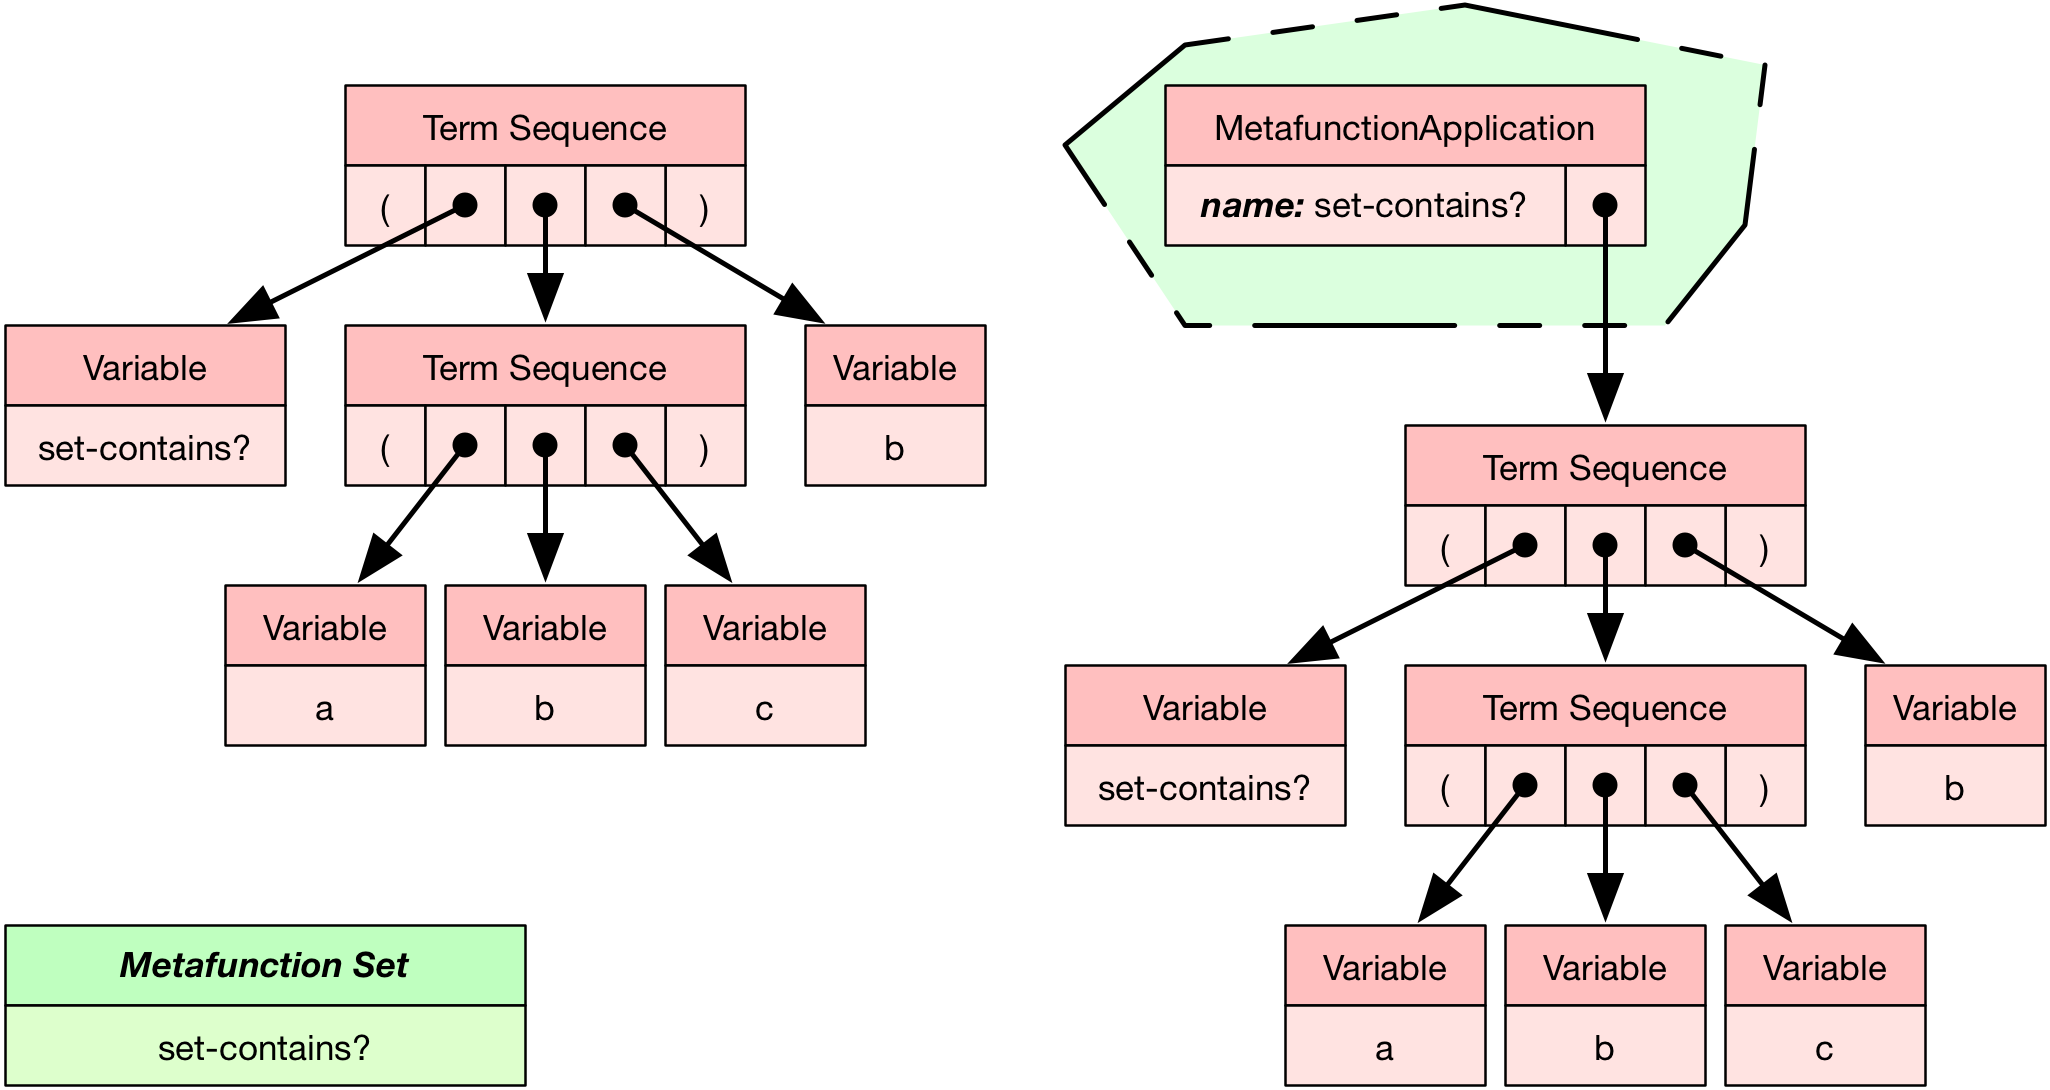
\includegraphics[scale=0.20]{transformation-term-mfapply.png}
\caption{Term-template before and after applying metafunctions.}
\label{transformation-term-mfapply}
\end{figure}

\section{Preprocessing Top-Level Forms}

Having defined and explained transformation/analysis passes for both patterns and term-templates, these are combined according to the needs of top-level forms. They are depicted in Figure \ref{transform-pipeline}. 

There are three different strategies that can be applied to patterns. Strategy \textbf{(a)} is applied to all patterns used in \texttt{define-language} form. Strategy \textbf{(b)} is applied to patterns used for domain/codomain testing of terms. Strategy \textbf{(c)} is applied to any other pattern. For term-templates, there's only a single transformation strategy.

\begin{figure}[ht]
\centering
	\makebox[\textwidth][c] { 
		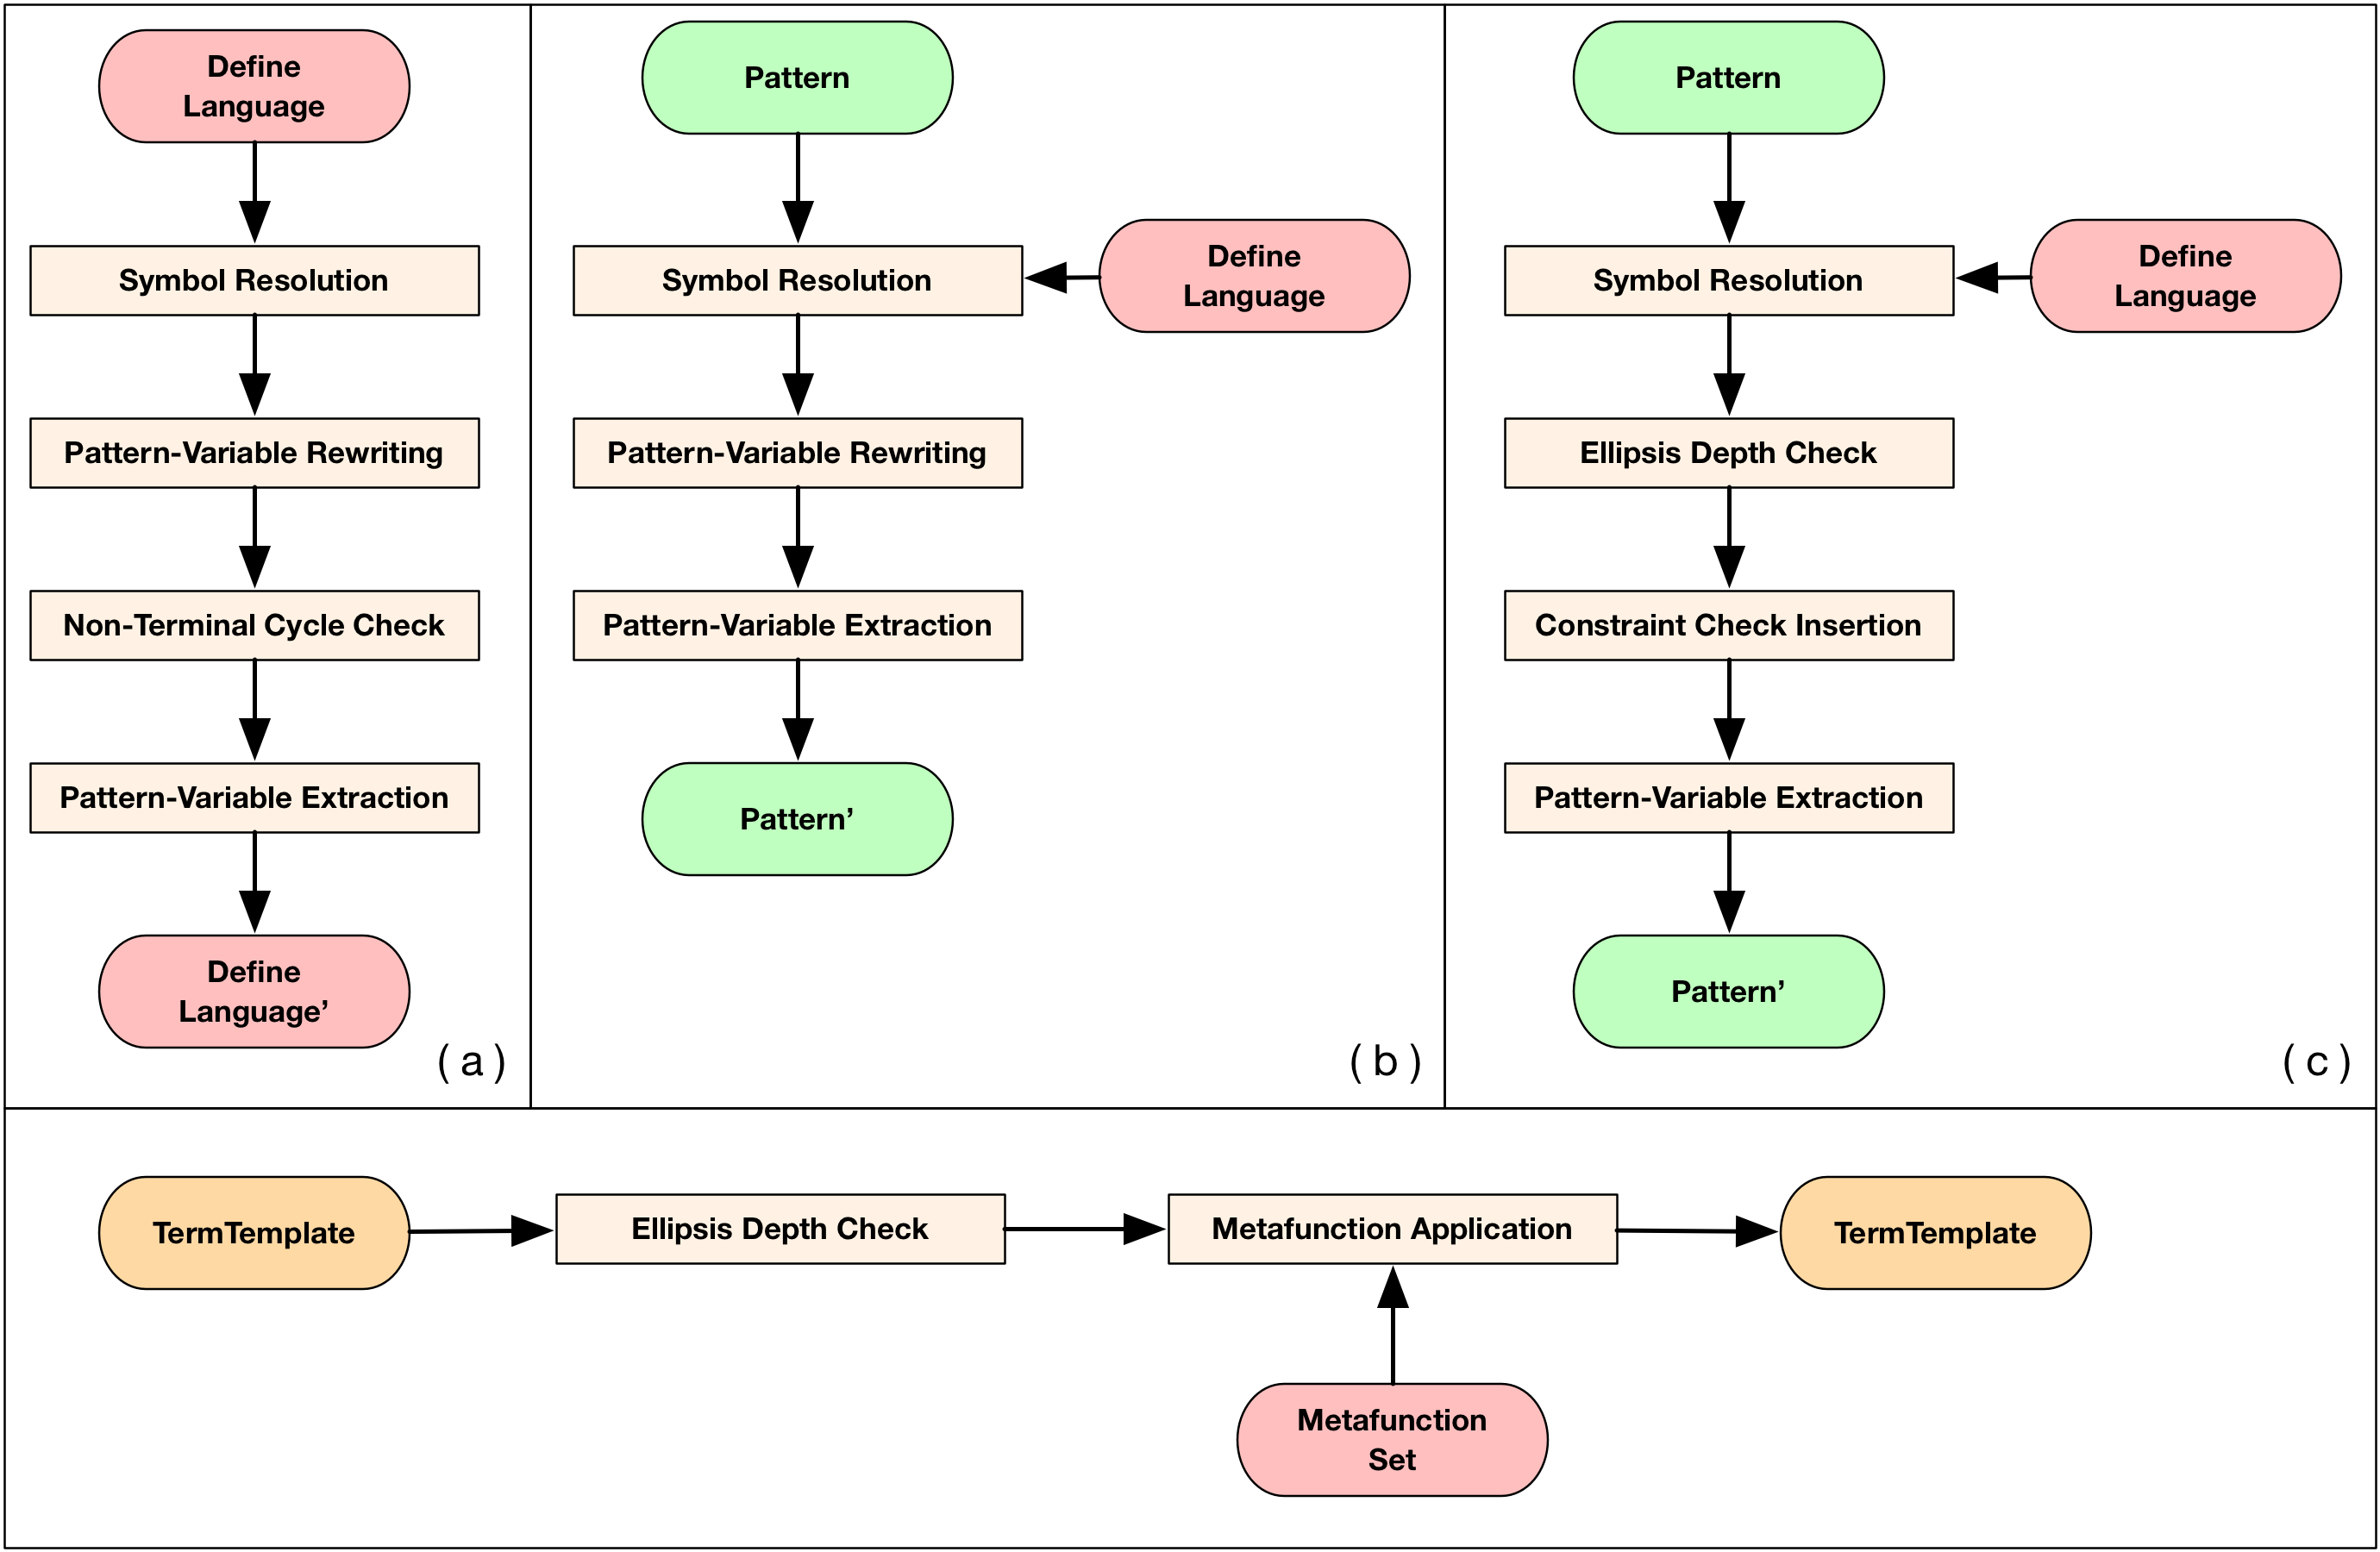
\includegraphics[scale=0.165]{transform-pipeline.png}
	}
	\caption{Transformations applied to patterns and term-templates.}
	\label{transform-pipeline}
\end{figure}


Notice that non-terminal resolution occurs with respect to non-terminal definitions on some \DefineLanguageNoArg \space form. Similarly, \textit{Metafunction Application} Pass requires the set $Mf$ containing all meta-functions defined until this point. 

\begin{enumerate}
\item All $tl=$\space \TlDefineLanguage \space forms. Maintain a set $L$ that stores ($n, tl$) pairs.
\item All $tl=$\space \TlDefineMetafunction \space forms. Maintain a set $M$ that stores $(n, tl)$ pairs.
\item All $tl=$\space \TlDefineReductionRelation \space forms. Maintain a set $R$ that contains $(n, tl)$ pairs.
\end{enumerate}

\subsection{Top-Level Form Analysis}

\begin{itemize}
\item
Given $tl=$\space \TlDefineLanguage
	\begin{enumerate}
		\item Apply strategy \textbf{(a)} to $tl$ resulting in $tl^{\prime}$.
		\item $L = L \cup \{ (n, tl^{\prime}) \}$
		\item Return $tl^{\prime}$.
	\end{enumerate}

\item $tl=$\space \TlDefineMetafunction:
	\begin{enumerate}
	\item Ensure that there exists a tuple $(l, df) \in L$, otherwise raise an Exception.
	\item Apply strategy \textbf{(b)} to $domain$ and $codomain$ patterns resulting in $domain^\prime$ and $codomain^\prime$.
	\item For each $mc_i=$ \MetafunctionCase, apply strategy \textbf{(c)} to $p$ thus resulting in $p^{\prime}$ and apply term-processing strategy to $t$ resulting in $t^{\prime}$. Let $mc_i^{\prime}$ = \MetafunctionCase[$p^{\prime}$][$t^{\prime}$].
	\item Let $tl^\prime$  = \TlDefineMetafunction[$n$][$l$][$domain^\prime$][$codomain^\prime$][$mc_1^\prime$][$mc_n^\prime$][false].
	\item $M = M \cup \{ (n, tl^\prime)\}$ and return $tl^\prime$.
	\end{enumerate}

\item $tl=$ \TlDefineReductionRelation:
\begin{enumerate}
\item Ensure that there exists a tuple $(l, df) \in L$ otherwise raise an Exception.
\item Apply strategy \textbf{(b)} to $domain$ pattern resulting in $domain^\prime$, if it exists.
\item For each $rc_i=$ \ReductionCase \space in $r$, apply strategy \textbf{(c)} to $p$ resulting in $p^{\prime}$ and apply the only term-processing strategy to $t$ resulting in $t^\prime$. Let $rc_i^\prime=$\space \ReductionCase[$p^{\prime}$][$t^{\prime}$][$n$][false].
\item Let $tl^\prime=$\space \TlDefineReductionRelation[$n$][$l$][$domain^\prime$][$rc_1^\prime$][$rc_n^\prime$]
\item $R = R \cup \{ (n, tl^\prime) \}$ and return $tl^\prime$.

\end{enumerate}

\item $tl=$ \ReadFromStdinAndApplyReductionRelation
\begin{enumerate}
\item If $f$ is present, ensure there exists a tuple $(f, mf) \in M$, otherwise raise Exception.
\item Ensure there exists a tuple $(r, red) \in R$, otherwise raise an Exception.
\item Return $tl$.
\end{enumerate}

\item
$tl=$ \RedexMatchAssertEqual.
	\begin{enumerate}
	\item Ensure that there exists a tuple $(l, df) \in L$, otherwise raise an Exception.
	\item Process $p$ according to strategy \textbf{(c)} resulting in $p^\prime$.
	\item Process $t$ according to the only specified strategy, resulting in $t^\prime$.
	\item For each $m_i=$\space \Match, process each $t_i$ according to the only specified strategy resulting in $t_i^\prime$. Let $m_i^\prime=$\space \Match[$s_1$][$t_1^\prime$][$s_n$][$t_n^\prime$][false].
	\item Let $tl^\prime=$\space\RedexMatchAssertEqual[$l$][$p^\prime$][$t^\prime$][$m_1^\prime$][$m_n^\prime$][false] and return $tl^\prime$.
	\end{enumerate}

\item $tl=$ \TermLetAssertEqual
	\begin{enumerate}
	\item  Process each $t_i$ according to the only specified strategy resulting in $t_i^\prime$.
	\item Process $t$ and $e$ according to the only specified strategy, resulting in $t^\prime$ and $e^\prime$, respectively.
	\item Let $tl^\prime=$\space \TermLetAssertEqual[$v_1$][$n_1$][$t_1^\prime$][$v_m$][$n_m$][$t_m^\prime$][$t^\prime$][$e^\prime$][false] and return $tl^\prime$.
	\end{enumerate}

\item $tl=$ \ApplyReductionRelationAssertEqual
	\begin{enumerate}
	\item Ensure that there exists a tuple $(r, red) \in R$, otherwise raise an Exception.
	\item Process $t$ according to the only specified strategy resulting in $t^\prime$
	\item Process each term $e_i$ according to the only specified strategy, resulting in $e_i^\prime$.
	\item Let $tl^\prime=$\space \ApplyReductionRelationAssertEqual[$r$][$t^\prime$][$e_1^\prime$][$e_n^\prime$][false] and return $tl^\prime$.
	\end{enumerate}
\end{itemize}

\subsection{Remarks}
It should be noted that the way in which PyPltRedex handles metafunction resolution is slightly different from PLTRedex. PLTRedex seems to keep track of metafunctions that have been defined up until a certain point, and it also keeps track of metafunctions that have not been defined yet. Roughly speaking, instead of passing a single set $Mf$ into "Metafunction Application Pass", PLTRedex passes a second set $\overline{Mf}$ containing names of metafunctions that haven't been defined yet. This way, when attempting to detect metafunction applications, "Metafunction Application Pass" also checks set $\overline{Mf}$ and raises \textbf{"cannot use metafunction before its definition"} error. Since PyPltRedex doesn't handle this at this time, all possible metafunction applications do not get rewritten and thus more often than not $codomain$ check fails.



\chapter{Code Generation}
\section{Notation}

A few words about notation; the original intent was to simply reuse Python code but it turned out to be not particularly space-friendly. Instead, to stay consistent with the notation described in Chapter \ref{chapter05}, the following notation for code-generation is used, as seen in the code snippet below.


\begin{minted}[tabsize=2,obeytabs,escapeinside=||,mathescape=true,fontsize=\normalsize]{pythoncomplexer.py:PythonCompLexer -x}

	
def |$f_p$|(match, term, head, tail):
	return None


\end{minted}

\begin{itemize}
\item Statements between \texttt{\{\%} and \texttt{\%\}} are Python statements executed by the compiler. Statements that are not, are generated RPython code.
\item Variables such as $f_p$ are \textit{meta-variables}; when a meta-variable is used in description of generated RPython code, an actual value assigned to it will be emitted instead.
\item Special \texttt{endfor}, \texttt{enddef}, \texttt{endif} are used to indicate an end of Python block.
\item Occasionally, there's a need for iterative Python statement generation, based on contents of a pattern or term-template. Array reference is used to retrieve fields of compile-time objects.

\end{itemize}

\section{Patterns}

\subsection{Introduction}

To be able to generate code for patterns, three kinds of functions are required.

\begin{enumerate}
\item
The \texttt{IsA} function that accepts a term and returns a boolean if it matches the desired pattern. This is done by ensuring that each term instance is of an expected class (e.g. \texttt{Integer}) and additionally verifying side conditions (e.g. \texttt{natural} term must be of class \texttt{Integer} and its value must be greater or equal to zero). All \texttt{IsA} functions have the following signature:

\begin{minted}[tabsize=2,obeytabs,escapeinside=||,mathescape=true,fontsize=\normalsize]{python}
isA(term: Term) -> boolean
\end{minted}

\item
The matching function that accepts a \texttt{Match} instance, a \texttt{Term} instance, and two extra arguments \texttt{head} and \texttt{tail}, which indicate a range of subterms in the term that haven't been matched yet. Successful matching increments value of \texttt{head} by one. In principle it should be possible to perform pattern matching bi-directionally but PyPltRedex doesn't implement this. All matching functions have the following signature:

\begin{minted}[tabsize=2,obeytabs,escapeinside=||,mathescape=true,fontsize=\normalsize]{python}
matchfunc(match: Match, term: Term, head: int, tail: int) -> [(Match, int, int)]
\end{minted}

\item
The top-level matching function that accepts a \texttt{Term} instance, initializes \texttt{Match} with pattern-variables found in the pattern and calls a matching procedure. \texttt{Match} instances are then filtered and returned. All top-level matching functions have the following signature:
\begin{minted}[tabsize=2,obeytabs,escapeinside=||,mathescape=true,fontsize=\normalsize]{python}
toplevel_matchfunc(term: Term) -> [Match]
\end{minted}
\end{enumerate}


\subsection{Is-A Functions}

\texttt{IsA} functions are generated for all built-in patterns excluding \texttt{InHole} patterns.  Originally, most of these procedures were generated by PyPltRedex dynamically but then I realized these could just the part of the runtime library introduced in Chapter \ref{chapter04}. This allowed for greater code generator simplification.

\begin{figure}[H]
\begin{minted}[tabsize=2,obeytabs,escapeinside=||,mathescape=true,fontsize=\normalsize]{python}
def term_is_number(term):
    return isinstance(term, Float) or isinstance(term, Integer)

def term_is_integer(term):
    return isinstance(term, Integer)

def term_is_float(term):
    return isinstance(term, Float)

def term_is_natural_number(term):
    return isinstance(term, Integer) and term.value() >= 0

def term_is_hole(term):
    return isinstance(term, Hole)

def term_is_string(term):
    return isinstance(term, String)

def term_is_boolean(term):
    return isinstance(term, Boolean)

def term_is_variable_not_otherwise_mentioned(term, variableset):
    return isinstance(term, Variable) and term.value() not in variableset
\end{minted}
\caption{\texttt{IsA} functions for all built-in datatypes.}
\label{codegen-builtin-isa}
\end{figure}

The figure above shows the \texttt{IsA} procedures for \texttt{number}, \texttt{real}, \texttt{natural}, \texttt{string}, \texttt{boolean} and \texttt{variable-not-otherwise-mentioned} patterns. All of these use Python's built-in \texttt{isinstance} function to check if a given term is of the proper subclass of \texttt{Term} described in Section \ref{section:runtime-terms}.

Most of these functions can be called directly. The only function that looks different is \texttt{term\_is\_variable\_not\_otherwise\_mentioned} and that is because a set of variables used by the related \texttt{define-language} form is required and is not known until compile time. This is solved by creating a wrapper function.

This completes the description of \texttt{IsA} functions. \texttt{IsA} functions are also generated for each non-terminal definition in a \texttt{define-language} form and their generation will be explained later.

\subsection{Matching Functions: Literals}
Matching $p=$\space \LiteralPattern \space is very similar to \texttt{IsA} functions described above. They first check if the passed \texttt{term} is of the expected class and then they compare the value of the term to the value $v$, passed in the place of \texttt{literal} parameter. These functions are also a part of the runtime library and can be seen in Figure \ref{codegen-pat-literal}.

\begin{figure}[ht]
\begin{minted}[tabsize=2,obeytabs,escapeinside=||,mathescape=true,fontsize=\normalsize]{python}
def consume_literal_integer(term, match, head, tail, literal):
    if isinstance(term, Integer) and term.value() == literal:
        return [ (match, head+1, tail) ]
    return []

def consume_literal_float(term, match, head, tail, literal):
    if isinstance(term, Float) and abs(literal - term.value()) < 0.001:
        return [ (match, head+1, tail) ]
    return []

def consume_literal_string(term, match, head, tail, literal):
    if isinstance(term, String) and term.value() == literal:
        return [ (match, head+1, tail) ]
    return []

def consume_literal_boolean(term, match, head, tail, literal):
    if isinstance(term, Boolean) and term.value() == literal:
        return [ (match, head+1, tail) ]
    return []

def consume_variable(term, match, head, tail, literal):
    if isinstance(term, Variable) and term.value() == literal:
        return [ (match, head+1, tail) ]
    return []
\end{minted}
\caption{Functions that match literals in a pattern.}
\label{codegen-pat-literal}
\end{figure}

Since functions do not conform to the previously described interface, a wrapper function is generated, calling one of the functions based on $kind$, as seen in Figure \ref{codegen-lit-code}.

\begin{figure}[ht]
\begin{minted}[tabsize=2,obeytabs,escapeinside=||,mathescape=true,fontsize=\normalsize]{pythoncomplexer.py:PythonCompLexer -x}

	
	
def |$f_p$|(match, term, head, tail):
	return |$consume_p$|(term, p[|$v$|])


\end{minted}
\caption{Generated function for a \LiteralPatternNoArg \space pattern}
\label{codegen-lit-code}
\end{figure}

\subsection{Matching Functions: Built-In Patterns and Non-terminals}

\begin{figure}[H]
\begin{minted}[tabsize=2,obeytabs,escapeinside=||,mathescape=true,fontsize=\normalsize]{pythoncomplexer.py:PythonCompLexer -x}

	
	
def |$f_p$|(match, term, head, tail):
	tmp0 = |$isa_p$|(term)
	if tmp0 == True:
		tmp1 = match.addtobinding(|$pv$|, term)
		head = head + 1
		return [(match, head, tail)]
return []


\end{minted}
\caption{Matching built-in patterns and non-terminal symbols.}
\label{codegen-builtin-nt-1}
\end{figure}

Given \BuiltInPattern \space or \space \NonTerminal \space and equipped with \texttt{IsA} functions defined above (also assuming \texttt{IsA} functions for non-terminal definitions have been generated), upon successful application of appropriate \texttt{IsA} procedure, \texttt{head} must be incremented by one and term must be assigned to the pattern-variable $pv$. The choice of \texttt{IsA} procedure depends on $t$.

Generated code does the following:

\begin{enumerate}
\item Call appropriate \texttt{IsA} procedure.
\item If the result is True, add the term to the \texttt{Match} instance under appropriate pattern-variable, increment \texttt{head} by one and return a list containing \texttt{(match, head, tail)} tuple.
\item Otherwise, return an empty list.
\end{enumerate}


\subsection{Matching Functions: Repeat}
\label{section:pattern-repeat}
Recall that patterns under ellipsis match lists of terms and can only be contained in pattern sequences and thus the \texttt{term} argument is always to be expected to be \newline \PatternSequence. Given $p=$ \PatternRepeat \space pattern, non-deterministic matching repetition of terms is handled in the following way. Let $pv_1^{(p)}, ..., pv_n^{(p)}$ be a set of pattern-variables assigned in $p_r$. These are read from the \newline \texttt{PatternVariables} annotation.  Let $f_p$ be the matching function for $p$ with usual parameters. Generate the matching function for $p_r$, $f_{p_r}$. Figure \ref{codegen-pattern-ellipsis-1} demonstrates this.

\begin{enumerate}
\item
For each symbol in $pv_i^{(p)}$, call \texttt{match.increasedepth} method. The functionality of \texttt{increasedepth} was described in Section \ref{section:Match}.
\item
Pack \texttt{match}, \texttt{head}, \texttt{tail} back into a tuple, and initialize lists \texttt{matches} and \texttt{queue} containing said tuple. \texttt{matches} will eventually contain all the matches produced by $f_p$. \texttt{queue} contains matches that are yet to be processed. Since $p_r$ can be non-deterministic, $f_{p_r}$ needs to be applied for every match in \texttt{queue}.
\item The following is repeated until \texttt{queue} is empty.
	\begin{enumerate}
	\item
	Remove \texttt{(m, h, t)} from the queue. If \texttt{h == t} then all elements of the sequence have been matched and there's nothing left to do.
	\item
	Retrieve an element at index the \texttt{head} of the term sequence and call $f_{p_r}$ with the resulting \texttt{Match} instance after calling \texttt{m.deepcopy}.
	\item Append the resulting list of matches to \texttt{matches} and \texttt{queue}.
	\end{enumerate}

\item
For each obtained \texttt{(m, h, t)} in \texttt{matches} call \texttt{m.decreasedepth} method with $pv_i^{(p)}$. This completes matching the list of terms. \texttt{matches} is returned.
\end{enumerate}

\begin{figure}[ht]
\begin{minted}[tabsize=2,obeytabs,escapeinside=||,mathescape=true,fontsize=\normalsize]{pythoncomplexer.py:PythonCompLexer -x}

	
	
	
def |$f_p$|(term, match, head, tail):
	:
	match.increasedepth(|$pv_i^{p}$|)
	
	matchtuple = (match, head, tail)
	matches, queue = [matchtuple], [matchtuple]
	while len(queue) != 0:
		m, h, t = queue.pop(0)
		if h == t: continue
		m = m.copy()
		newmatches = |$f_{p_r}$|(term.get(h), m, h, t)
	matches, queue = matches + newmatches, queue + newmatches
	for (m, h, t) in matches:
	:
		m.decreasedepth(|$pv_i^{p}$|)
	
	return matches

\end{minted}
\caption{Matching repetition of terms \RepeatNoArg \space in \texttt{Sequence}.}
\label{codegen-pattern-ellipsis-1}
\end{figure}


\subsection{Matching Functions: PatternSequence}
Given $p=$\space \PatternSequence, generate matching functions $f_{p_1}, ..., f_{p_n}$ for patterns $p_1, ..., p_n$. Code generation for pattern sequences is more involved and requires a bit of setup.

\begin{enumerate}
\item
First, ensure that the \texttt{term} is a \texttt{Sequence}.  Then, the term has to be "entered" to be ready for matching; that is, to be able to use $f_{p_i}$ to match subterms, new values for \texttt{head} and \texttt{tail} are required. Initialize \texttt{nhead = 0} and set \texttt{ntail} to be length of the term sequence - these will be used to track which elements of the \texttt{Sequence} haven't been matched yet.
\item Before matching elements of the term, ensure that the number of these elements is greater or equal to the number of elements in the \texttt{PatternSequence}, excluding patterns under ellipses and constraint checking nodes.
\item \texttt{Sequence} is now ready to be matched - create an empty list of matches and initialize it with \texttt{(match, ntail, nhead)} tuple.
\item
Depending on the kind of pattern $p_i$, different matching strategies are required and are to be explained later. For now, assume all the patterns $p_i$ have been matched.
\item
After matching all patterns $p_i$, \texttt{TermSequence} has to be "exited"; that is, the original \texttt{head} and \texttt{tail} have to be restored. Let \texttt{matches\_m} be a list of matches after matching the last pattern $p_n$. For each resulting match tuple (m, h, t) in \texttt{matches\_m}, ensure that \texttt{h = t}, that is all terms in \texttt{TermSequence} have been matched. If that is the case, tuple \texttt{(m, head+1, tail)} is appended to the list of resulting matches, indicating that \texttt{TermSequence} itself has been matched.
\end{enumerate}
Figure \ref{codegen-pattern-seq-1} demonstrates this.

\begin{figure}[htb]
\centering
\begin{minted}[tabsize=2,obeytabs,escapeinside=||,mathescape=true,fontsize=\normalsize]{pythoncomplexer.py:PythonCompLexer -x}

	
	
	
def |$f_p$|(term, match, head, tail):
	if not isinstance(term, Sequence): return []
	subtail, subhead = 0, term.length()
	if subtail - subhead < |$n$| : return []
	|$matches_0$|= [(match, subtail, subhead)]
	
		
			#snip
		
			#snip
		
			#snip
		
	outmatches = []
	for m, h, t in matches_m:
		if m == t:
			outmatches.append((m, head+1, tail))
	return outmatches

\end{minted}
\caption{Setting up \texttt{Sequence} for pattern matching.}
\label{codegen-pattern-seq-1}
\end{figure}

Now, different code is emitted for different kinds of $p_i$.

\begin{itemize}
\item $p_i=$ \PatternRepeat. The matching function $f_{p_i}$ is called with \texttt{term} (i.e. \texttt{Sequence}) for each \texttt{(m,h,t)} in $matches_{i-1}$. Results of matching is accumulated into list $matches_{i}$. Additionally, ensure that the remaining number of terms in the \texttt{Sequence} is greater than the remaining number of non-optional patterns to be matched; that is $n-i$. Matches that pass this test are accumulated into the list $matches_{i+1}$ Finally, ensure that $matches_{i+1}$ is non-empty, otherwise return an empty list. Figure \ref{codegen-pattern-seq-2} demonstrates this.

\begin{figure}[htb]
\centering
\begin{minted}[tabsize=2,obeytabs,escapeinside=||,mathescape=true,fontsize=\normalsize]{pythoncomplexer.py:PythonCompLexer -x}

	
|$matches_i$| = []
for m, h, t in |$matches_{i-1}$|:
	|$matches_i$| = |$matches_i$| + |$f_{p_i}$|(term, m, h, t)
	
	
		
|$matches_{i+1}$| = []
for m, h, t in |$matches_{i}$|:
	if tail - head >= |$r$|:
		|$matches_{i+1}$|.append((m, h, t))
if len(|$matches_{i+1}$|) == 0: return []
	
\end{minted}
\caption{Matching \RepeatNoArg \space in \texttt{Sequence}.}
\label{codegen-pattern-seq-2}
\end{figure}

\item $p_i=$ \PatternCheckConstraint. For each \texttt(m, h, t) in $matches_{i-1}$, ensure that \texttt{m.comparekeys} succeeds for $sym_1$ and $sym_2$ and accumulate succeding matches into $matches_{i}$. Additionally, check if list $matches_{i}$ is non-empty otherwise return. Figure \ref{codegen-pattern-seq-3} demonstrates this.


\begin{figure}[htb]
\centering
\begin{minted}[tabsize=2,obeytabs,escapeinside=||,mathescape=true,fontsize=\normalsize]{pythoncomplexer.py:PythonCompLexer -x}

	
|$matches_i$| = []
for m, h, t in |$matches_{i-1}$|:
	if m.comparekeys(|$sym_1$|, |$sym_2$|):
		|$matches_i$|.append((m, h, t))
if len(|$matches_i$|) == 0: return []
\end{minted}
\caption{Handling \ConstraintCheckNoArg \space while matching \texttt{Sequence}.}
\label{codegen-pattern-seq-3}
\end{figure}

\item Any other pattern kind $p_i$, given a list of matches $matches_{i-1}$, call $f_{p_i}$ for each \texttt{(m, h, t)} in $match_{i-1}$ with term at position \texttt{h} and accumulate resulting matches into new list $match_{i}$. If $match_{i}$ is empty, matching \texttt{TermSequence} has failed and empty list is returned. Figure \ref{codegen-pattern-seq-4} demonstrates this.

\begin{figure}[htb]
\begin{minted}[tabsize=2,obeytabs,escapeinside=||,mathescape=true,fontsize=\normalsize]{pythoncomplexer.py:PythonCompLexer -x}


|$matches_i$| = []
for m, h, t in |$matches_{i-1}$|:
	|$matches_i$| = |$matches_i$| + |$f_{p_i}$|(term.get(h), match, h, t)
if len(|$matches_i$|) == 0: return []

\end{minted}
\caption{Handling any another pattern in \PatternSequenceNoArg \space while matching \texttt{Sequence}.}
\label{codegen-pattern-seq-4}
\end{figure}
\end{itemize}

\subsection{Match Functions: InHole}
Given pattern \PatternInHole, let $f_p^{(impl)}$ be the name of the function for \texttt{in-hole} pattern. Recall that the \texttt{in-hole} pattern is annotated with pattern-variables during \textit{Pattern Variable Extraction} Pass described in Section \ref{section:pv-extraction}. Let $pv_i^{(p_1)}$ and $pv_i^{(p_2)}$ be annotations for $p_1$ and $p_2$. Finally, generate functions for $p_1$ and $p_2$ and let them be $f_{p_1}$ and $f_{p_2}$ respectively.

Notice that this function contains an extra parameter \texttt{path}, which is used to keep track of a path to a possible \texttt{hole}. To conform to the established interface, a wrapper function will be generated later.

Since $p_1$ and $p_2$ are self-contained patterns with possible non-deterministic behavior, \texttt{match} cannot be passed to $f_{p_1}$ and $f_{p_2}$ as is. Instead, create special \texttt{Match} instances to be passed to $f_{p_1}$ and $f_{p_2}$ that are initialized with $pv_i^{(p_1)}$ or $pv_i^{(p_2)}$ accordingly.

First, call $f_{p_2}$ with the appropriate match, if the resulting list of matches is non-empty, do the following: (1) append the current term to the path; (2) call the path copying function thus replacing the term with \texttt{hole} and (3) call $f_{p1}$ with an appropriate \texttt{match}. If the resulting set of matches is not empty, increment \texttt{head} (without overwriting it!) by one signaling successful matching of the \texttt{in-hole} pattern, combine resulting matches of $f_{p_1}$ and $f_{p_2}$ with the initial \texttt{match} as explained in Section \ref{section:Match}, and append to \texttt{matches}.

If the given \texttt{term} is \texttt{Sequence}, continue matching the \texttt{in-hole} pattern. Each element of the sequence is added to the path, $f_p^{(impl)}$ is called with said element, resulting matches are added to \texttt{matches}, and topmost term in the \texttt{path} is popped. Resulting \texttt{matches} are returned. This logic is shown in Figure \ref{pat-inhole-1}.

\begin{figure}[!htb]
\begin{minted}[tabsize=2,obeytabs,escapeinside=||,mathescape=true,fontsize=\normalsize]{pythoncomplexer.py:PythonCompLexer -x}

	
	
	
	
	def |$f_p^{(impl)}$|(term, match, head, tail, path):
	matches = []
	p2match = Match([|$pv_1^{(p_2)}, ..., pv_m^{(p_2)}$|])
	p2ms = |$f_{p_2}$|(term, p2match, 0, 1)
	if len(p2ms) != 0:
		p1match = Match(|$pv_1^{(p_1)}, ..., pv_n^{(p_1)}$|)
		npath = path + [term]
		nterm = copy_path_and_replace_last(tmp0, hole)
		p1ms = |$f_{p_1}$|(nterm, p1match, 0, 1)
		if len(p1ms) != 0:
			nhead = head + 1
			ms = match_cartesian_product_add_binding_to(
				p1ms, p2ms, match, nhead, tail)
			matches = matches + ms
	if isinstance(term, Sequence):
		path.append(term)
		for i in range(term.length()):
			childterm = term.get(i)
			results= |$f_p^{impl}$|(childterm, match, head, tail, path)
			matches = matches + results
		path.pop()
	 return matches
# continued below
\end{minted}
\caption{Code for \PatternInHoleNoArg \space pattern.}
\label{pat-inhole-1}
\end{figure}

Finally, to get rid of the \texttt{path} parameter from the signature of $f_p^{(impl)}$, a wrapper function $f_p$ is generated. Additionally, it also handles constraint checks $c_i$ if applicable. Since constraint checks are optional, there are two cases to consider.

\begin{enumerate}
\item No constraint checks - simply return \texttt{matches}
\item Constraint checks are present - for each \PatternCheckConstraint \space generate a call to the \texttt{comparekeys} method with $sym_1$ and $sym_2$. This is done for each \texttt{Match} instance returned by calling $f_p^{(impl)}$.
\end{enumerate}

\begin{figure}[!htb]
\begin{minted}[tabsize=2,obeytabs,escapeinside=||,mathescape=true,fontsize=\normalsize]{pythoncomplexer.py:PythonCompLexer -x}
# continued from above.
	
def |$f_p$|(term, match, head, tail):
	matches = |$f_p^{(impl)}$|(match, head, tail, [])
	
	nmatches = []
	for m, h, t in matches:
		
	if not m.comparekeys(|$s_1$|, |$s_2$|):
		continue
		
	nmatches.append((m, h, t))
	return nmatches
	
	return matches
	
	

\end{minted}
\caption{Generation of wrapper function for \PatternInHoleNoArg \space pattern, continued from Figure \ref{pat-inhole-1}.}
\label{pat-inhole-2}
\end{figure}

\subsection{Top-Level Matching Functions}
Given some pattern $p$, generating a top-level function for a pattern involves the following steps:

\begin{itemize}
\item Retrieve a set of pattern-variables $pv_1^{p}, ..., pv_n^{p}$ assigned in the pattern from the annotation \texttt{PatternVariables}.
\item Retrieve a set of pattern-variables $pvr_1^{p}, ..., pvr_m^{p}$ that are to be removed after matching from annotation \texttt{PatConstraintCheckRemoveVars} (see Section \ref{section:constraint-check}).
\item Let $f_p$ be the top-level function for pattern $p$.
\item Generate matching function $f_p^{(match)}$ for pattern $p$.
\end{itemize}

Now, we get to the code-generation. Initialize the \texttt{Match} object with pattern-variables $pv_i^{p}$ and call $f_p$ with said \texttt{Match} instance, set \texttt{head} and \texttt{tail} to zero and one, respectively. After a list of matches is returned, strip out the resulting \texttt{Match} from \texttt{(Match, int, int)}  tuples as well as remove symbols $pvr_i^{p}$ from the \texttt{Match} instances. Resulting \texttt{Match} instances are appended to an array. The array is then returned.


\begin{figure}
\begin{minted}[tabsize=2,obeytabs,escapeinside=||,mathescape=true,fontsize=\normalsize]{pythoncomplexer.py:PythonCompLexer -x}

	
	
	
	
def |$f_p$|(term):
	match = Match(|$pv_1^{p}, ..., pv_n^{p}$|)
	matches = |$f_p^{(match)}$|(term, match, 0, 1)
	ret = []
	for m, h, t in matches:
	
		m.removekey(|$pvr_i^{(p)}$|)
		ret.append(m)
	
	return ret

\end{minted}
\caption{Generation of top-level matching function for pattern $p$.}
\label{pat-toplevel}
\end{figure}

\subsection{Repeat: Example}

Given pattern \texttt{((n ...) ...)} (\texttt{n} is shorthand for \texttt{number}) and term \texttt{((1 2 3)())}, the matching algorithm should return a \texttt{Match} instance pattern-variable assignment \texttt{n = ((1 2 3) ())}. The diagram below shows how using the \texttt{increasedepth} and \texttt{decreasedepth} methods provided by `Match` facilitate the matching.

\begin{figure}[h]
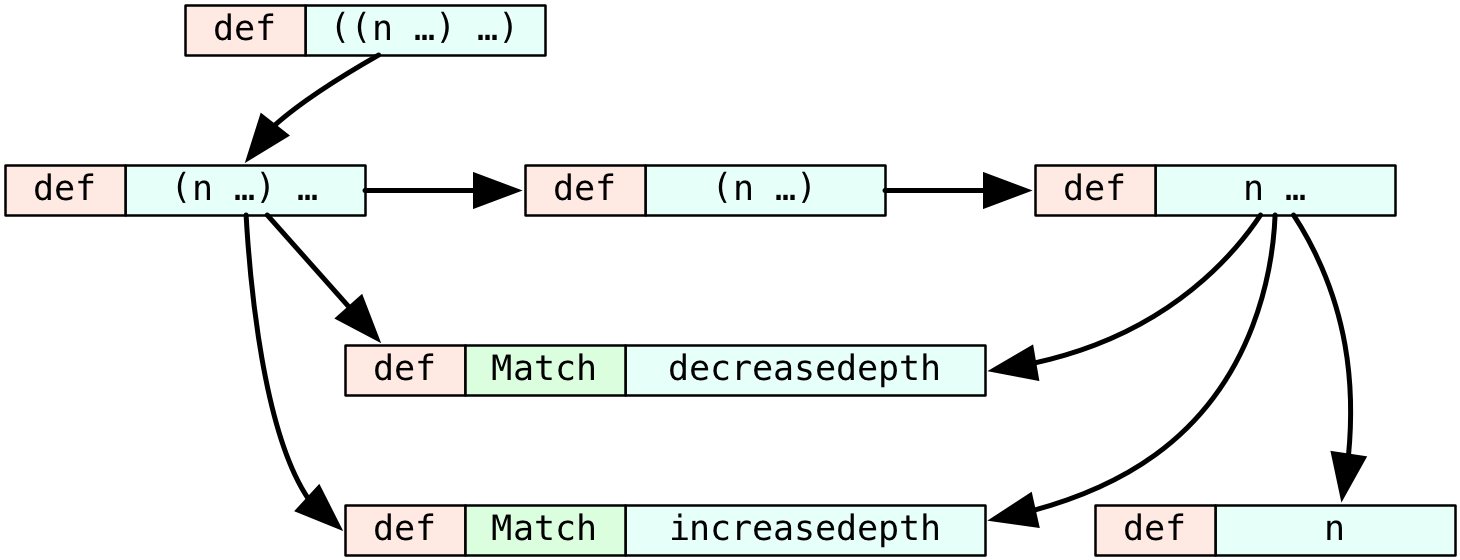
\includegraphics[scale=0.25]{ellipsis-example-callgraph.png}
\caption{Callgraph for function matching pattern \texttt{((n ...) ...)}}
\label{ellipsis-example-callgraph}
\end{figure}

Callgraph for the function matching the pattern \texttt{((n ...) ...)} can be seen in Figure \ref{ellipsis-example-callgraph}. Code generation algorithm generates five matching functions for this pattern:

\begin{enumerate}
\item function for pattern \texttt{((n ...) ...)}
\item function for pattern \texttt{(n ...) ...}
\item function for pattern \texttt{(n ...) }
\item function for pattern \texttt{n ... }
\item function for pattern \texttt{n}
\end{enumerate}

Figure \ref{ellipsis-example-fig-a} shows the state of the \texttt{Match} object before beginning to match a term (red nodes) against a pattern (blue nodes). Outlined pattern nodes represent the current sub-pattern being matched; and since matching hasn't begun yet the entire pattern is outlined. The same applies to the term. Initially, the \texttt{Binding} instance assigned to the pattern-variable \texttt{n} in the \texttt{Match} instance has an empty stack.

Figure \ref{ellipsis-example-fig-b} shows the state of the \texttt{Match} object after entering the function for \textit{outer} ellipsis and calling the \texttt{increasedepth("n")} method. This pushes an empty \texttt{Sequence} onto the stack.


Figure \ref{ellipsis-example-fig-c} shows the state of the \texttt{Match} object after entering the generated function for \textit{inner} ellipsis and calling the \texttt{increasedepth("n")} method. This pushes an empty \texttt{Sequence} onto the stack. The \texttt{Binding} for pattern-variable $n$ now contains two \texttt{Sequence} instances on the stack.

Figure \ref{ellipsis-example-fig-d} shows the matching of term \texttt{Integer(1)}. \texttt{addtobinding} method is called with \texttt{"n"} and \texttt{Integer(1)} as arguments. Since the topmost term on the stack is \texttt{Sequence}, \texttt{Integer(1)} is appended to it.

Figures \ref{ellipsis-example-fig-e} and \ref{ellipsis-example-fig-f} call \texttt{addtobinding} with \texttt{Float(2.01)} and \texttt{Integer(3)}. Both terms are appended to the topmost \texttt{Sequence} on the stack.

All terms in \texttt{Sequence} have been consumed. Figure \ref{ellipsis-example-fig-g} shows the state of the match object after calling \texttt{decreasedepth("n")}. Since the stack contains two \texttt{Sequence} instances, the topmost one is removed from stack and appended to the first \texttt{Sequence}. Function for \textit{inner} ellipsis is exited.

Now, the remaining empty term sequence has to be matched, as seen in Figure \ref{ellipsis-example-fig-h}.

Figure \ref{ellipsis-example-fig-i} shows the state of the \texttt{Match} object after entering the generated function for \textit{inner} ellipsis. An empty \texttt{Sequence} instance is pushed onto the stack.

Since the term sequence is empty, the function for the \texttt{number} pattern cannot be called. Figure \ref{ellipsis-example-fig-j} shows the state of the \texttt{Match} object after calling \texttt{decreasedepth("n")}. Since the stack contains two \texttt{Sequence} instances, the topmost one is popped from the stack and appended to the previous \texttt{Sequence}. The function for \textit{inner} ellipsis is exited.

Finally, there are no more terms to match in the outermost sequence and \texttt{decreasedepth("n")} has to be called, as shown in Figure \ref{ellipsis-example-fig-k}. Since the stack only contains a single term, no action is performed. The \texttt{Match} contains assignment \texttt{n = ((1 2 3)())}, as expected.

One may notice that this example doesn't cover non-determinism when matching patterns under ellipsis. When matching term \texttt{(1 2 3)} against pattern \texttt{n ...} (as shown in Figures \ref{ellipsis-example-fig-d}, \ref{ellipsis-example-fig-e}, \ref{ellipsis-example-fig-f}), the matches shown in Figure \ref{ellipsis-example-matches-1} are returned. To obtain these matches, the \texttt{(n ...)} pattern has to be "entered" first, thus setting values of \texttt{head} and \texttt{tail} to zero and the length of \texttt{Sequence}, respectively. Then, pattern \texttt{n ...} is matched in the way explained above (i.e. \texttt{increasedepth}, match pattern \texttt{n}, \texttt{decreasedepth}), resulting in matches in Figure \ref{ellipsis-example-matches-1}.  Now, when exiting the function for the pattern \texttt{(n ...)}, the only acceptable match among the four is the one whose \texttt{head=tail}.

After matching pattern \texttt{(n\ ...)}, the control flow (see callgraph in Figure \ref{ellipsis-example-callgraph}) returns to the function that matches pattern \texttt{(n\ ...)\ ...}, and the only returned match is added to the queue. The queue at this point contains a single match. This match is dequeued, and the function for pattern \texttt{(n\ ...)} is called with term \texttt{()}. \texttt{head} and \text{tail} are set to zero and the function for pattern \texttt{n\ ...} is called. \texttt{increasedepth} is called. Since term \texttt{()} contains no numbers, the only possible match returned by this function is shown in Figure \ref{ellipsis-example-matches-2}.

Finally, the \textit{outer} ellipsis produces matches shown in Figure \ref{ellipsis-example-matches-3}. When returning from the function for pattern \texttt{((n\ ...)\ ...)}, two of the matches are discarded because \texttt{head != tail}.


\begin{figure}[!htb]
\makebox[\textwidth][c] { 
	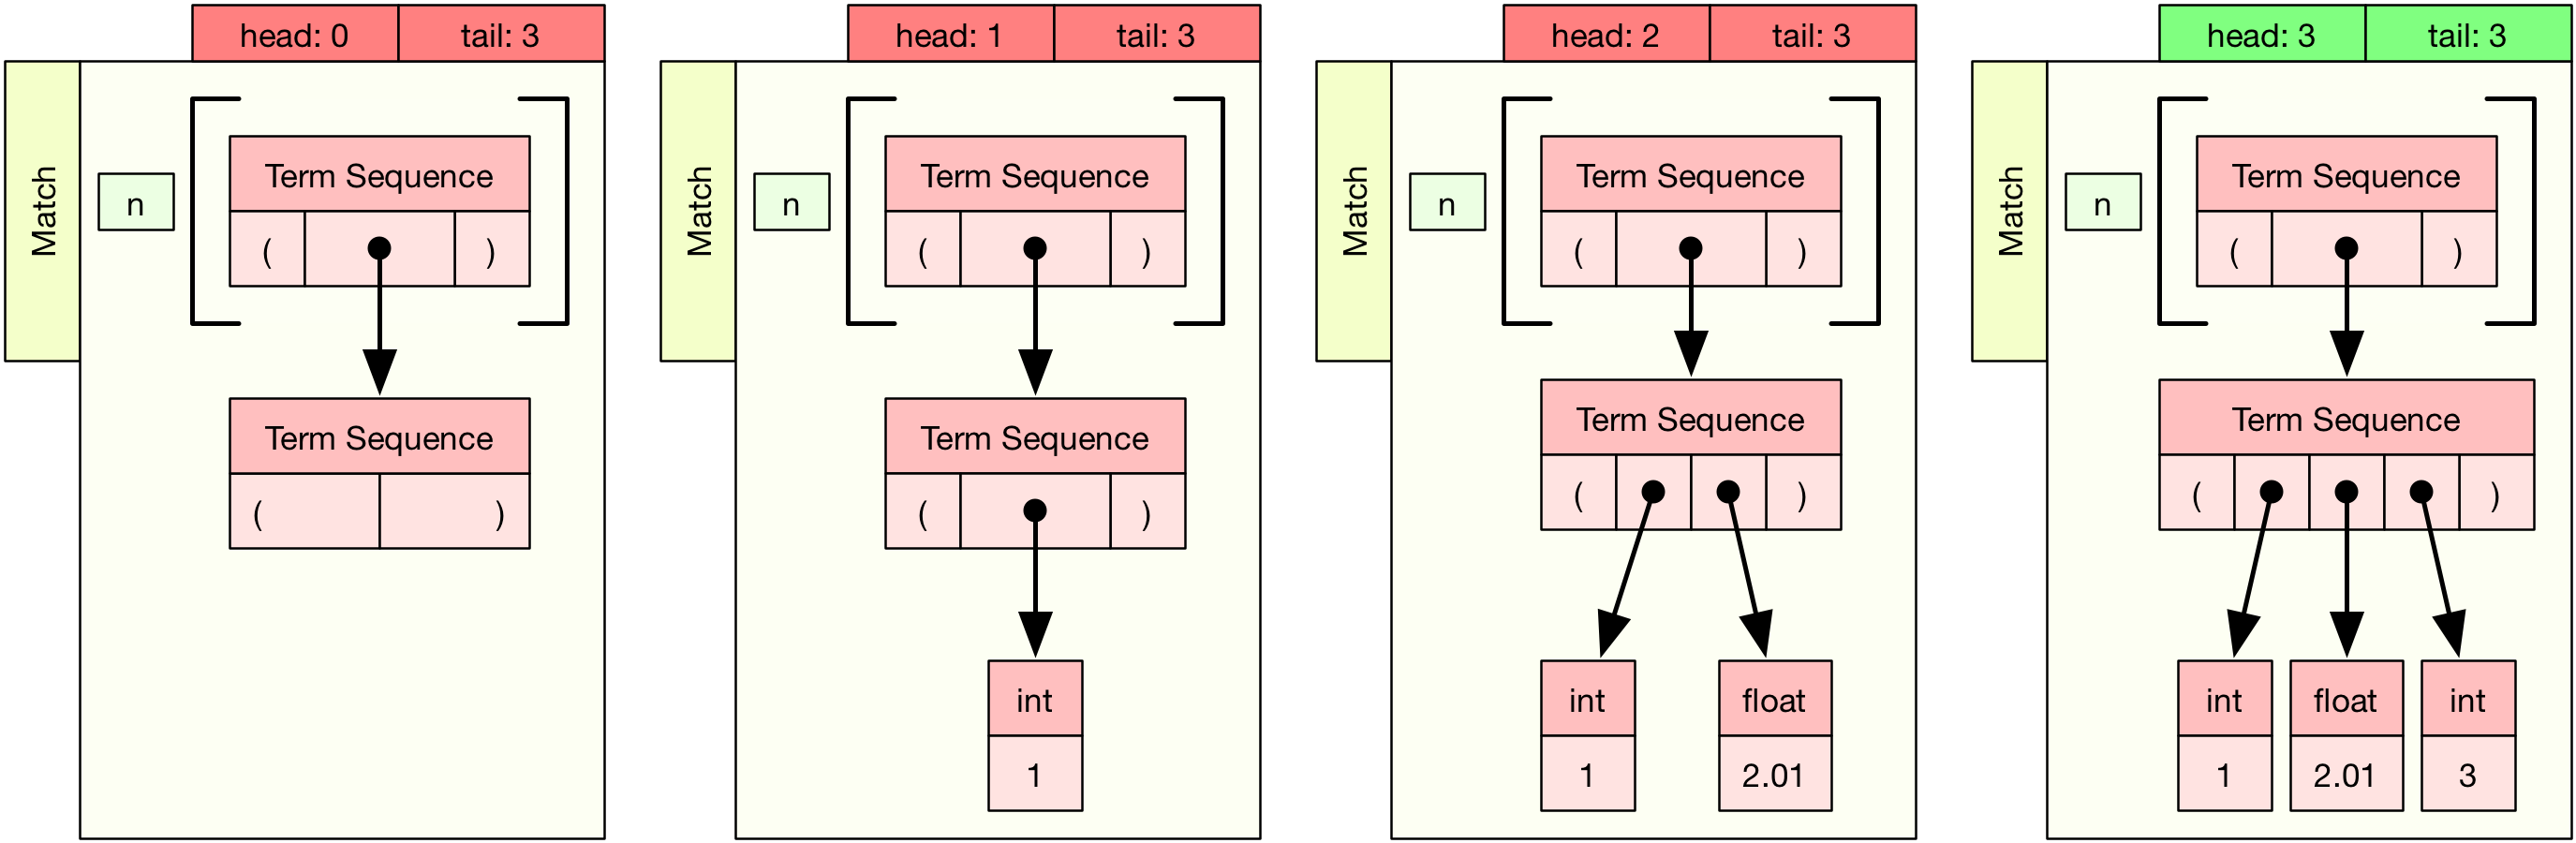
\includegraphics[scale=0.152]{ellipsis-example-matches-1.png}
}
\caption{Matches returned after matching term \texttt{(1 2 3)} against pattern \texttt{n ...}}
\label{ellipsis-example-matches-1}
\end{figure}

\begin{figure}[H]
\caption{Lifetime of \texttt{Match} object}
%\begin{adjustwidth}{-1cm}{1cm}

\makebox[\textwidth][c] { 
	\fbox{
		\begin{subfigure}{0.5\linewidth}
			\raisebox{5mm}{
				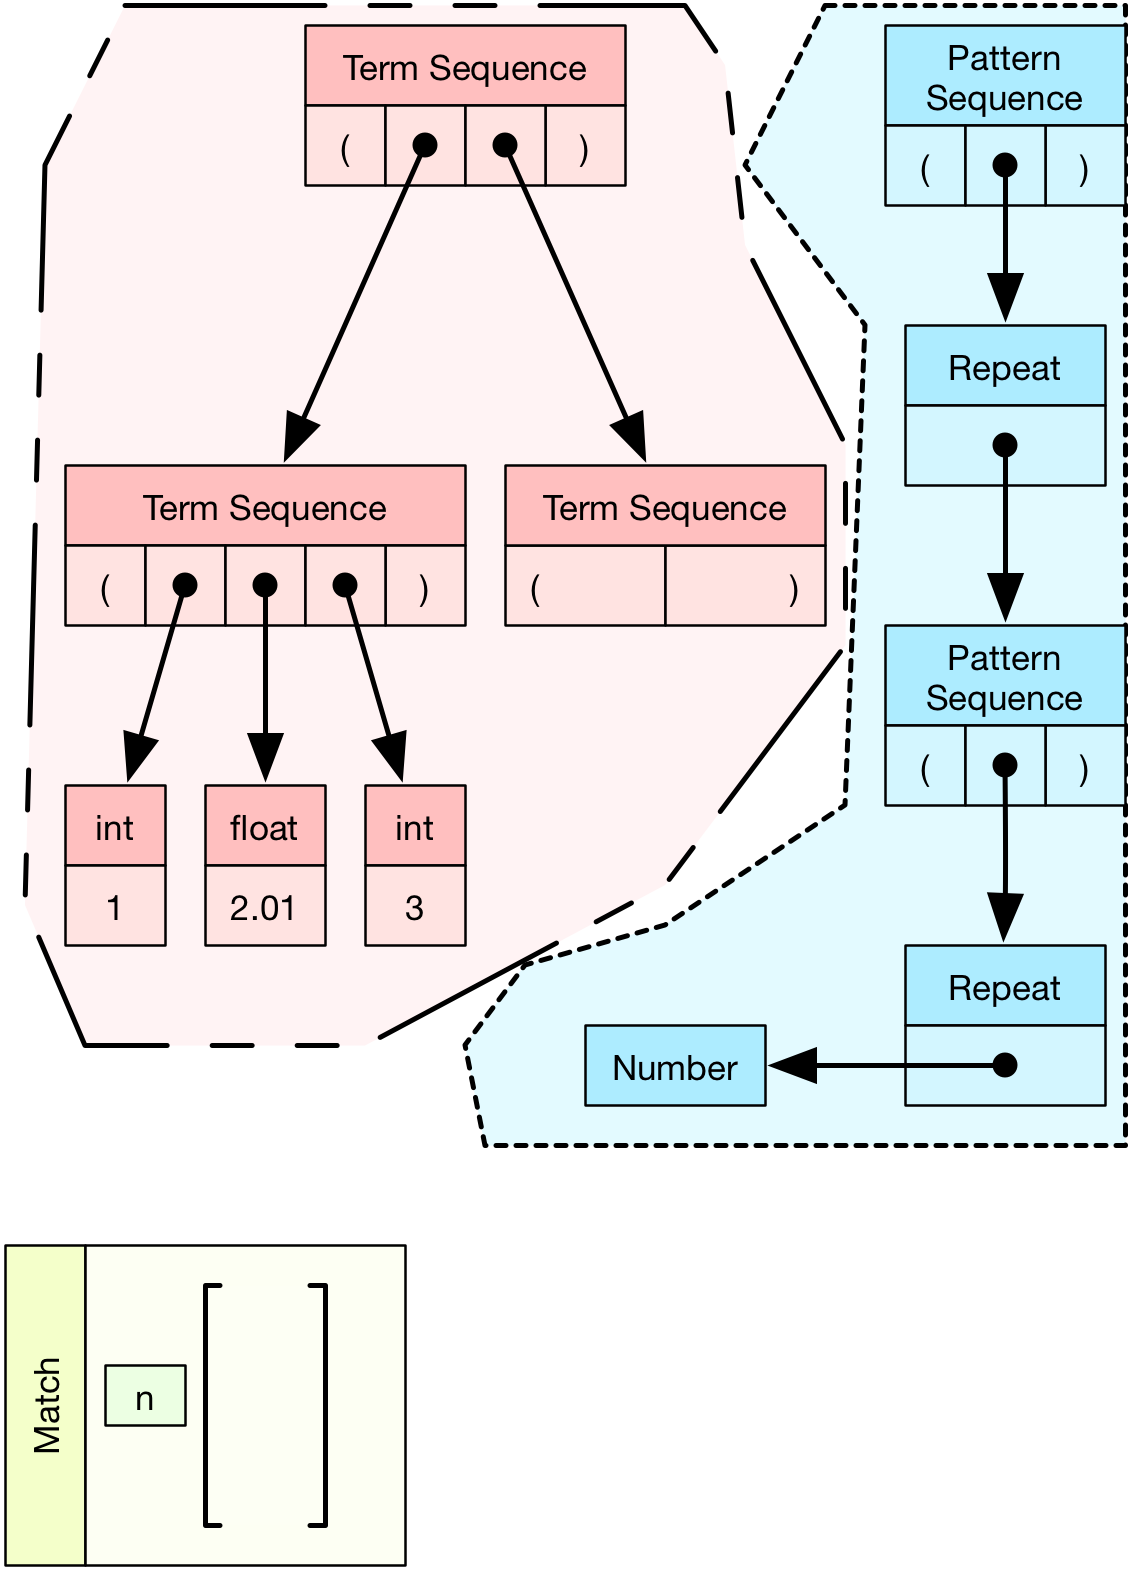
\includegraphics[scale=0.152]{ellipsis-example-fig-a.png}
			}
			\caption{Before matching the pattern.}
			\label{ellipsis-example-fig-a}
		\end{subfigure}
		\begin{subfigure}{0.5\linewidth}
			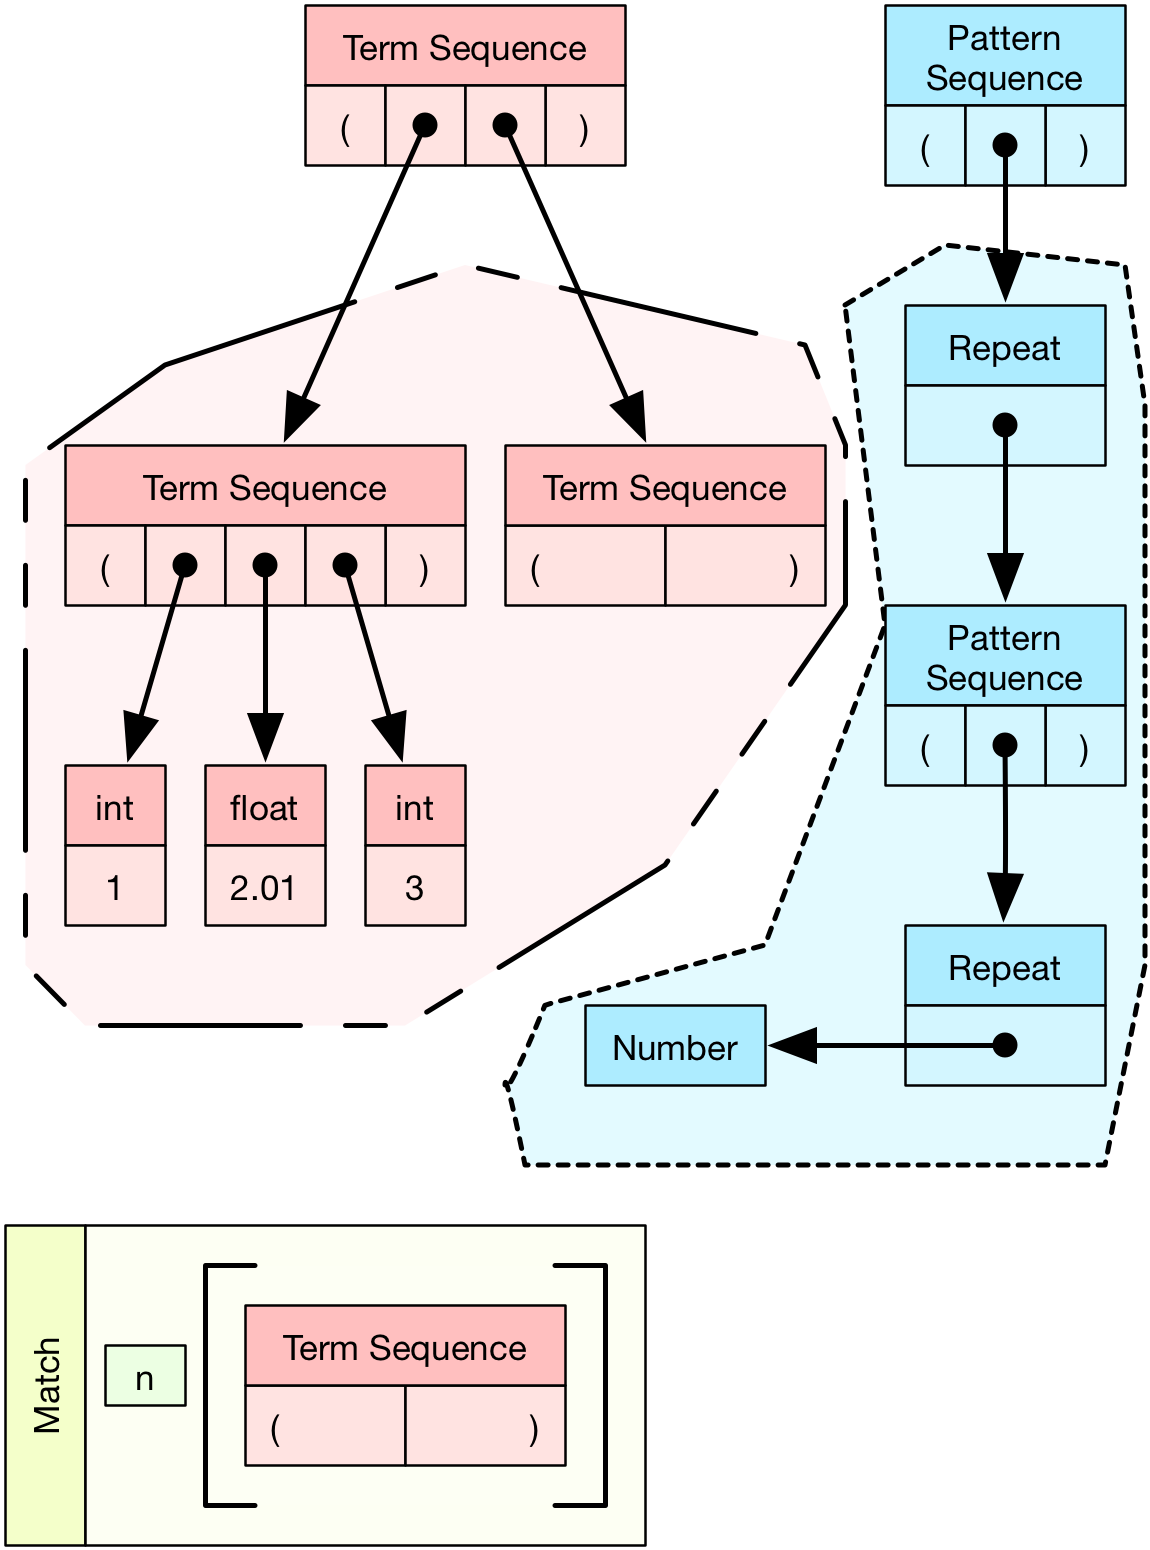
\includegraphics[scale=0.152]{ellipsis-example-fig-b.png}
			\vspace*{+11mm}
			\caption{Enter outer ellipsis and \texttt{increasedepth("n")}.}
			\label{ellipsis-example-fig-b}
		\end{subfigure}
	}
}

\makebox[\textwidth][c] { 
	\fbox{
		\begin{subfigure}{0.5\linewidth}
			\raisebox{19mm}{
				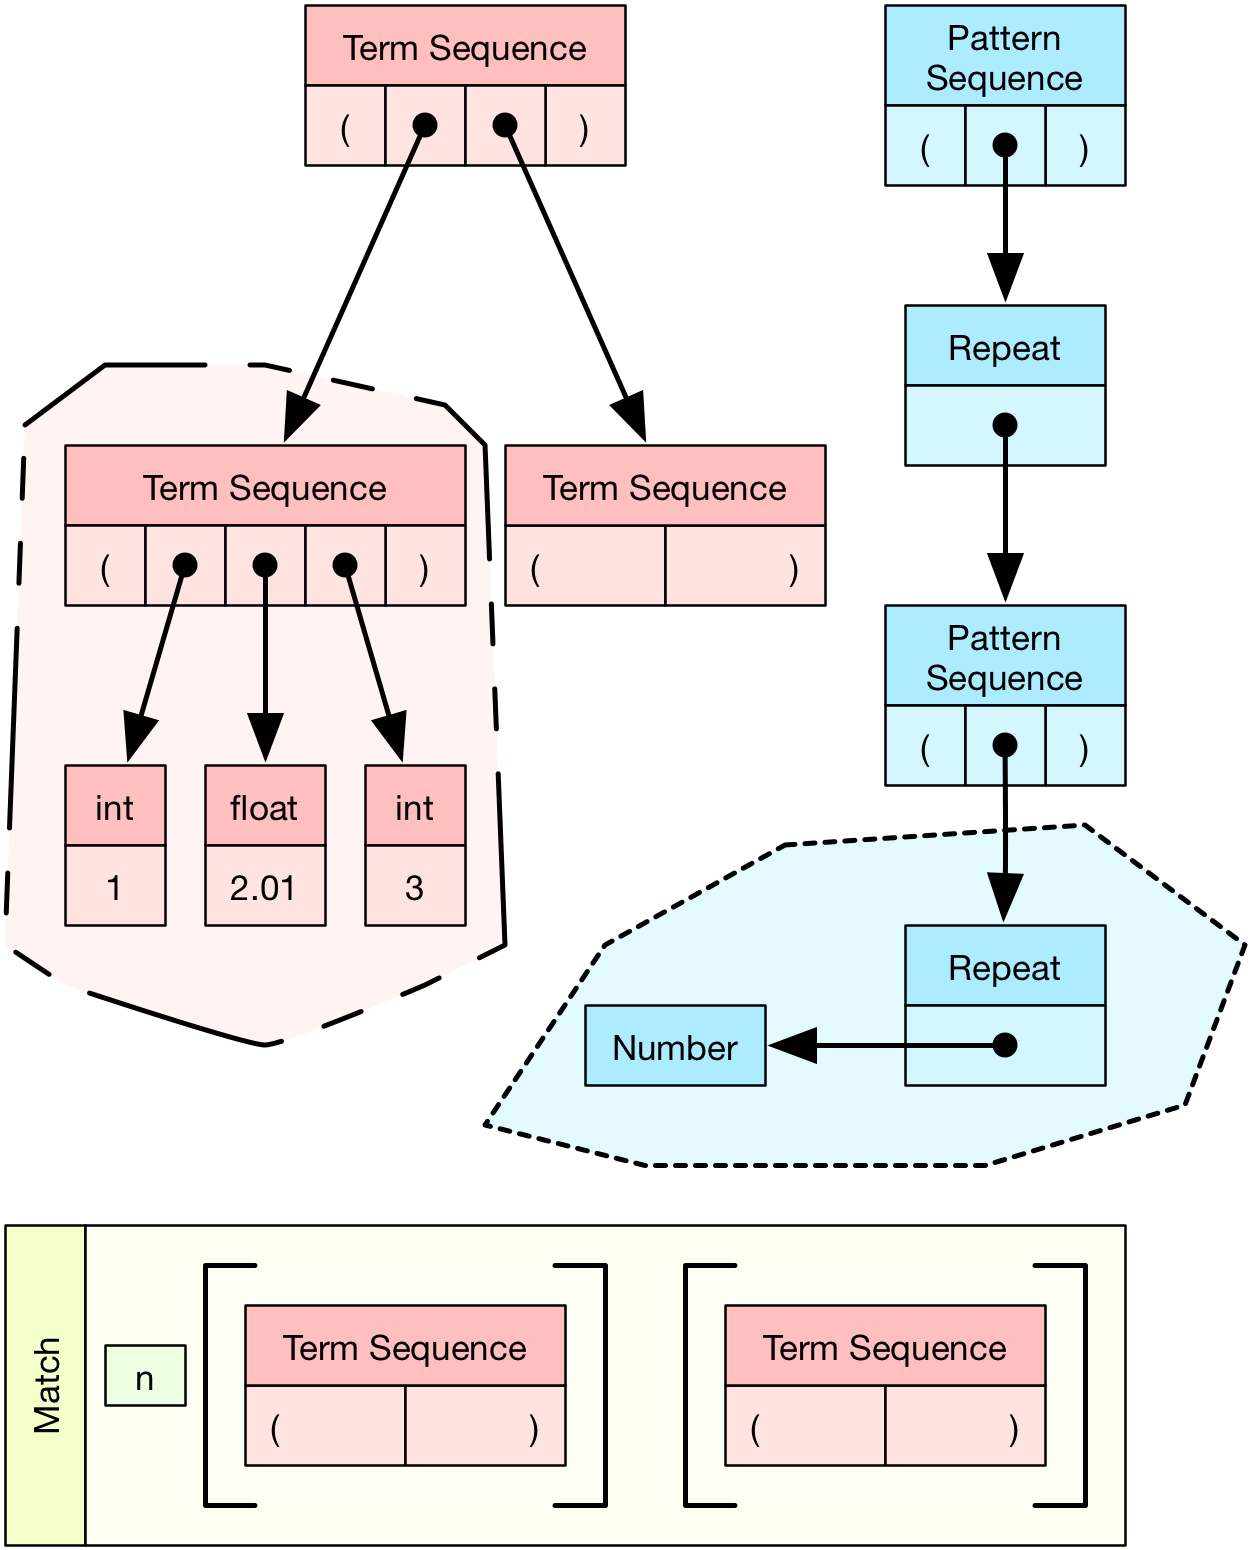
\includegraphics[scale=0.152]{ellipsis-example-fig-c.png}
			}
			\caption{Enter inner ellipsis and \texttt{increasedepth("n")}.}
			\label{ellipsis-example-fig-c}
		\end{subfigure}
		\begin{subfigure}{0.5\linewidth}
			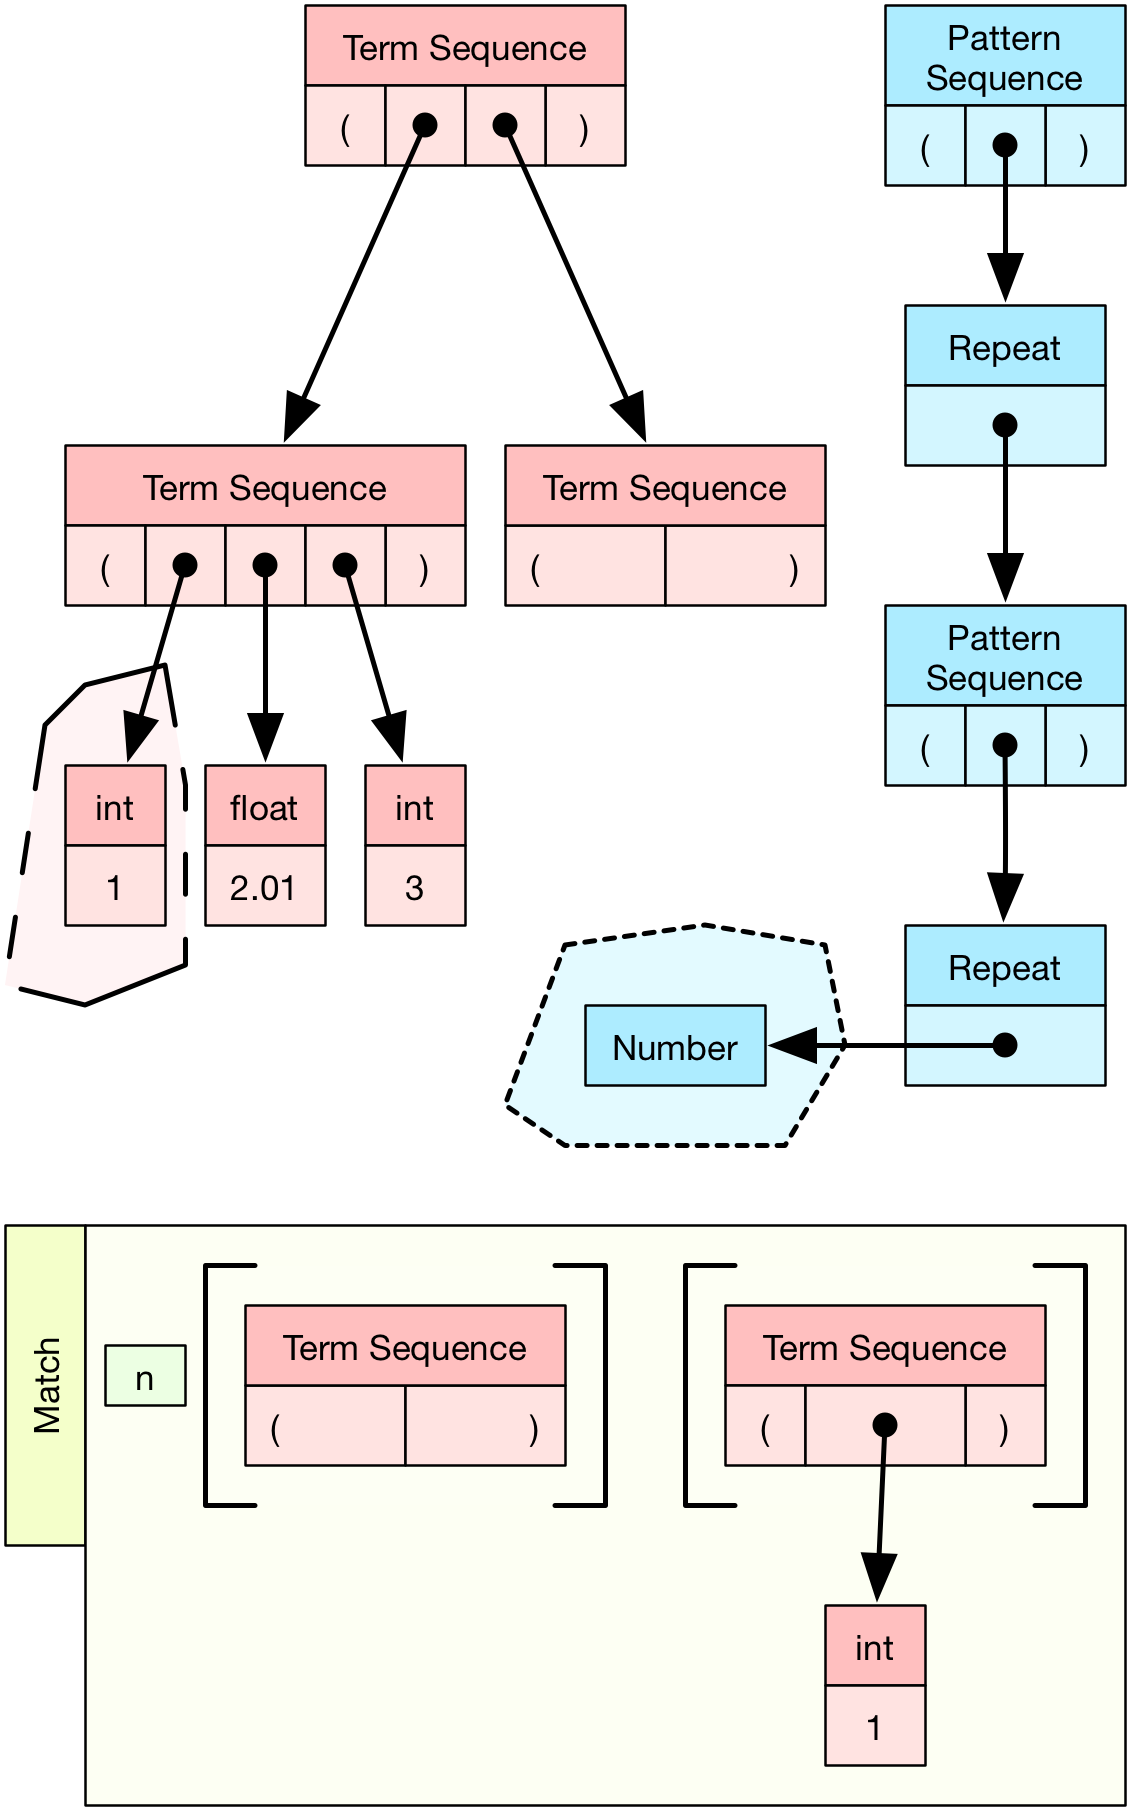
\includegraphics[scale=0.152]{ellipsis-example-fig-d.png}
			\caption{\texttt{addtobinding("n", Integer(1))}}
			\label{ellipsis-example-fig-d}
		\end{subfigure}
	}
}

%\end{adjustwidth}
\end{figure}

\begin{figure}[H]\ContinuedFloat

\makebox[\textwidth][c] { 
	\fbox{
		\begin{subfigure}{0.5\linewidth}
			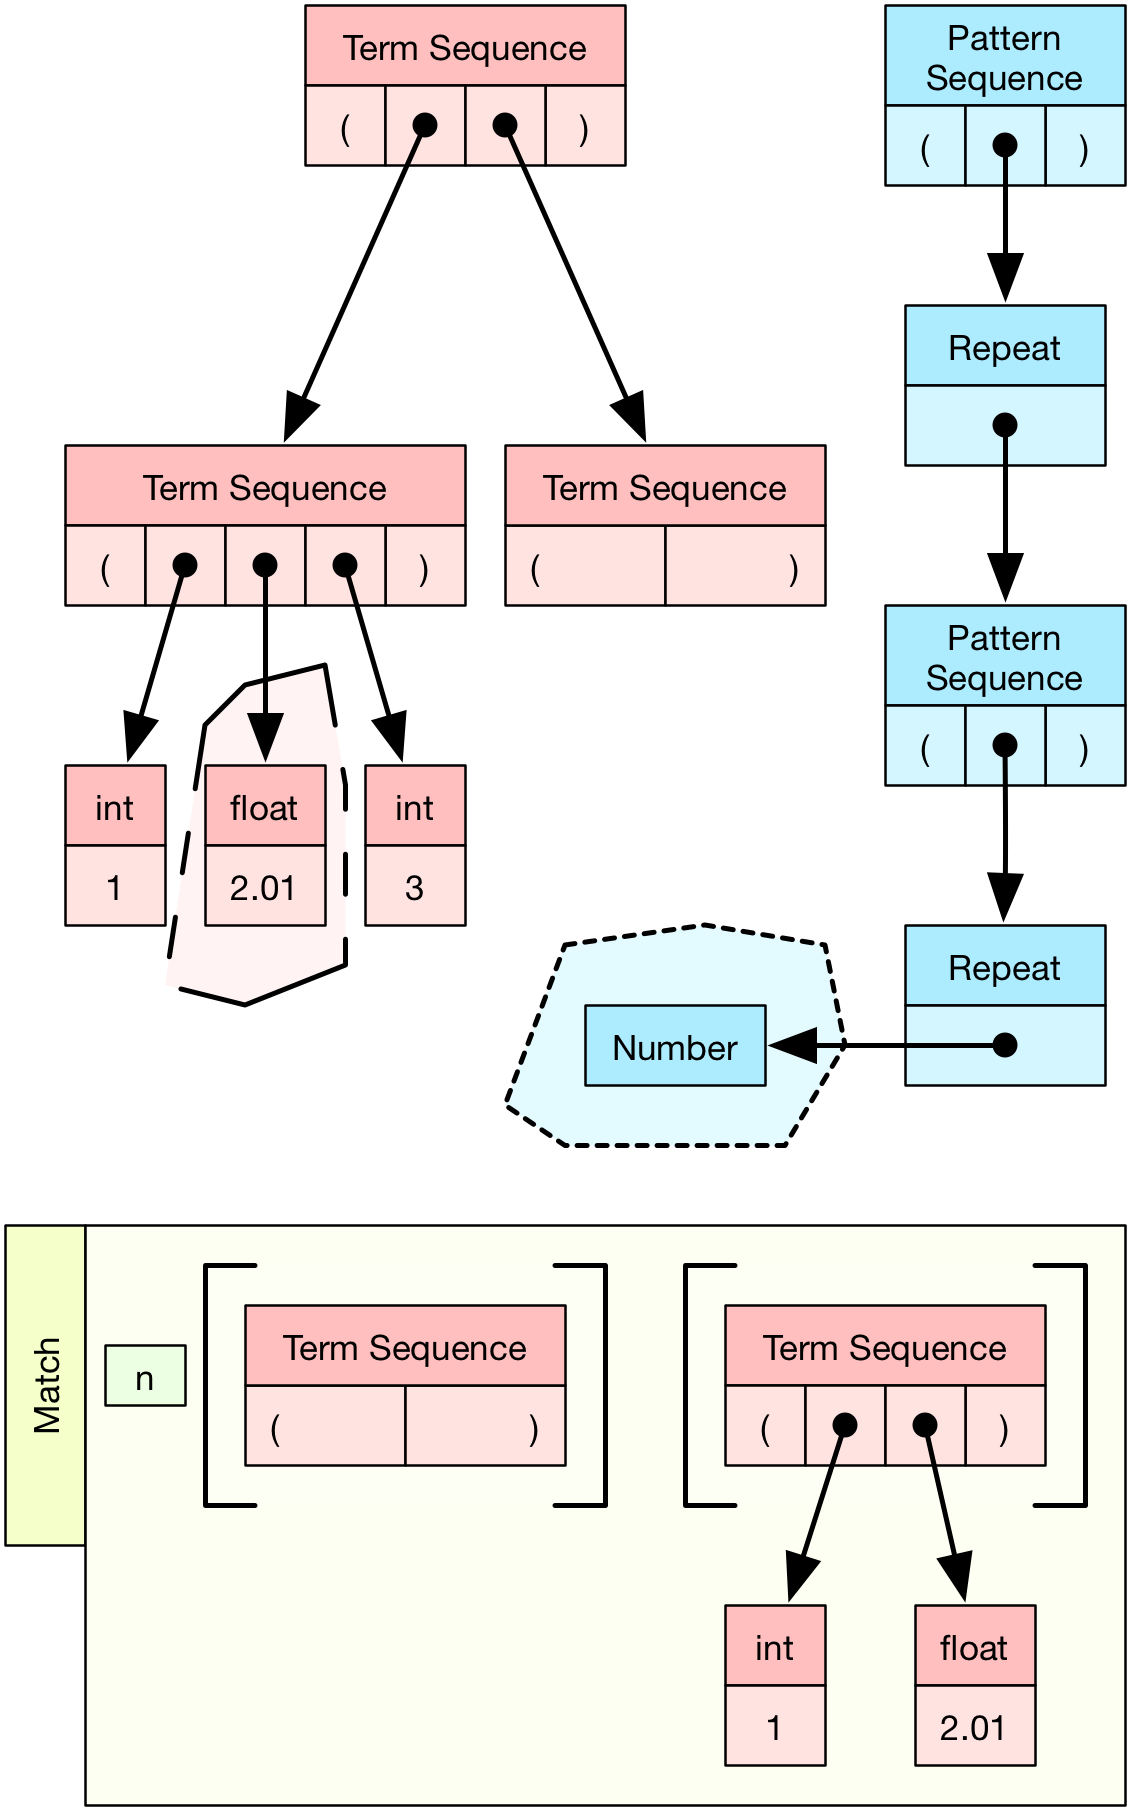
\includegraphics[scale=0.152]{ellipsis-example-fig-e.png}
			\caption{\texttt{addtobinding("n", Float(2.01))}}
			\label{ellipsis-example-fig-e}
		\end{subfigure}
		\begin{subfigure}{0.5\linewidth}
			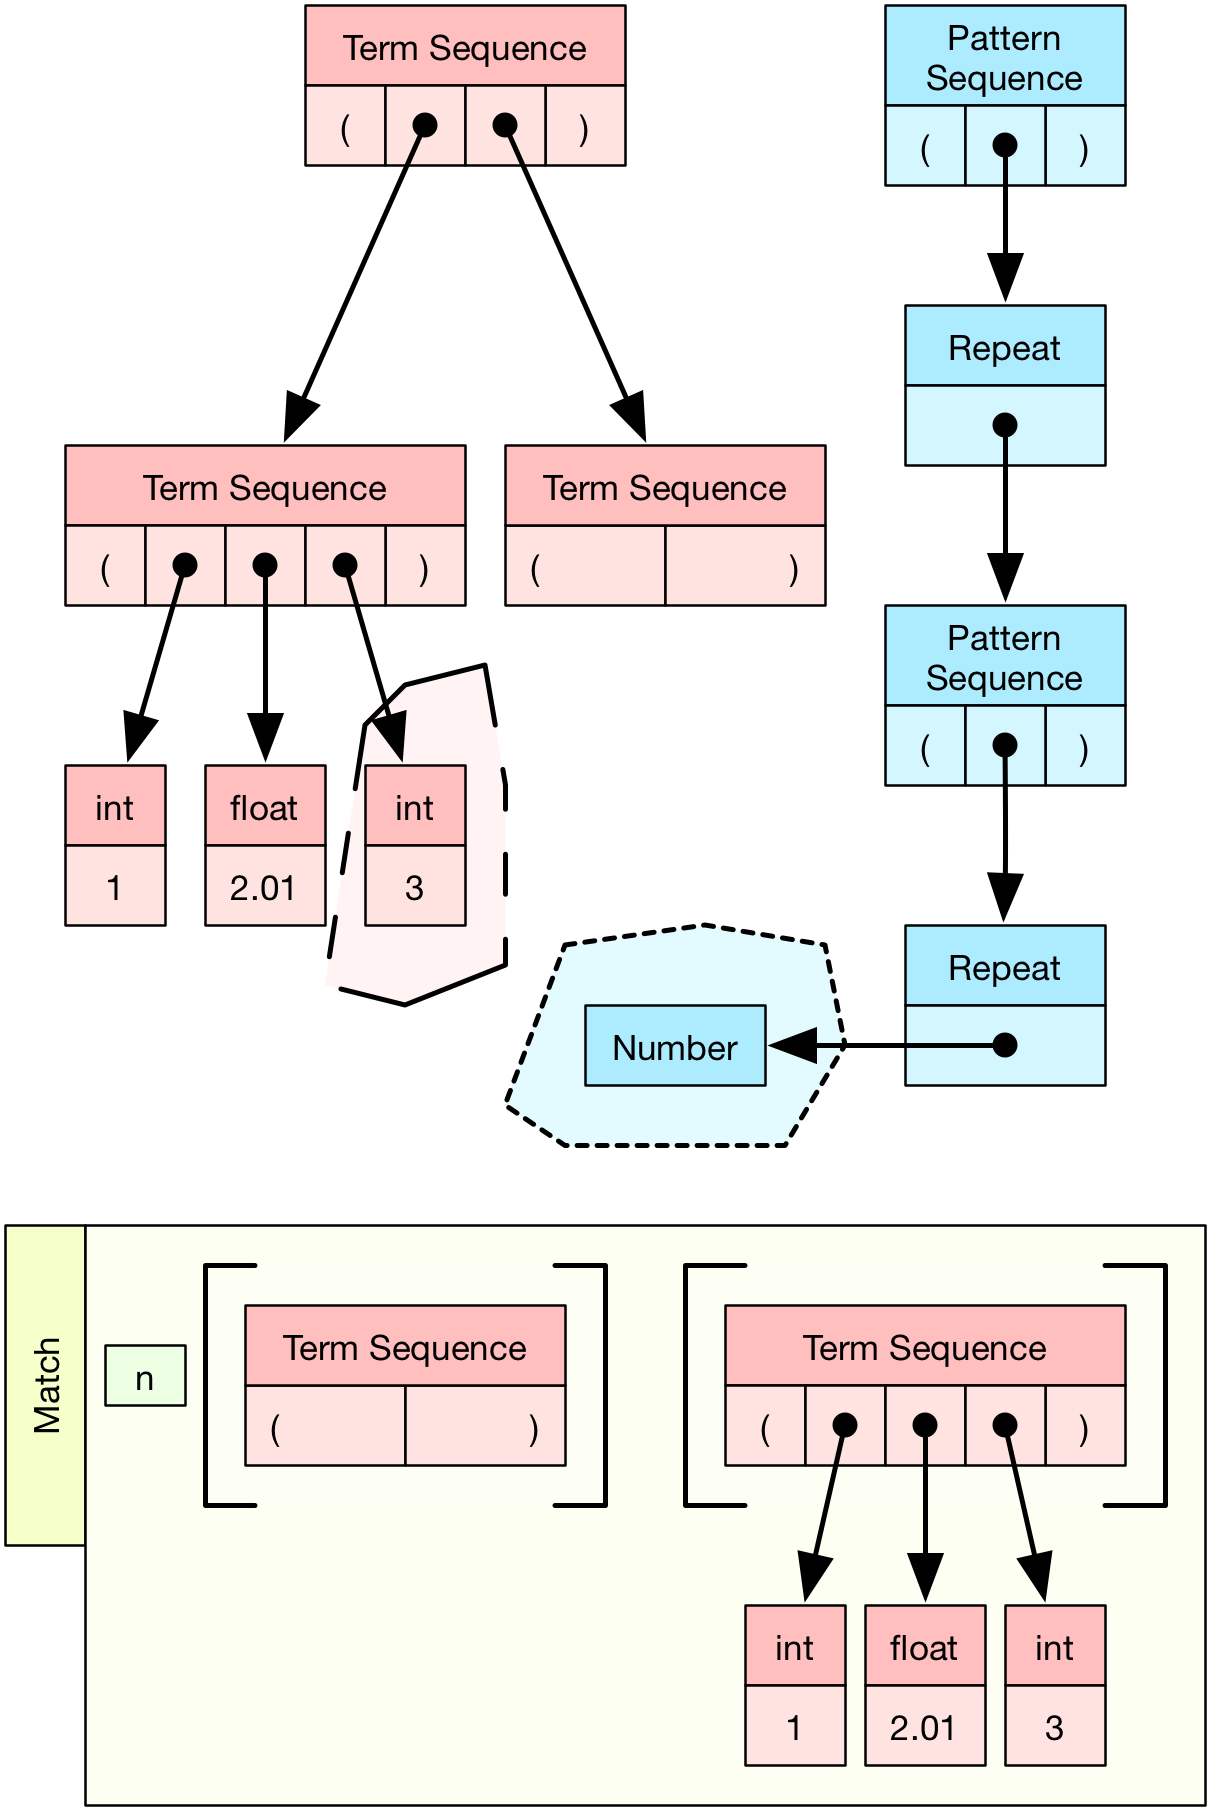
\includegraphics[scale=0.152]{ellipsis-example-fig-f.png}
			\caption{\texttt{addtobinding("n", Integer(3))}}
			\label{ellipsis-example-fig-f}
		\end{subfigure}
	}
}

\makebox[\textwidth][c] { 
	\fbox{
	\begin{subfigure}{0.5\linewidth}
		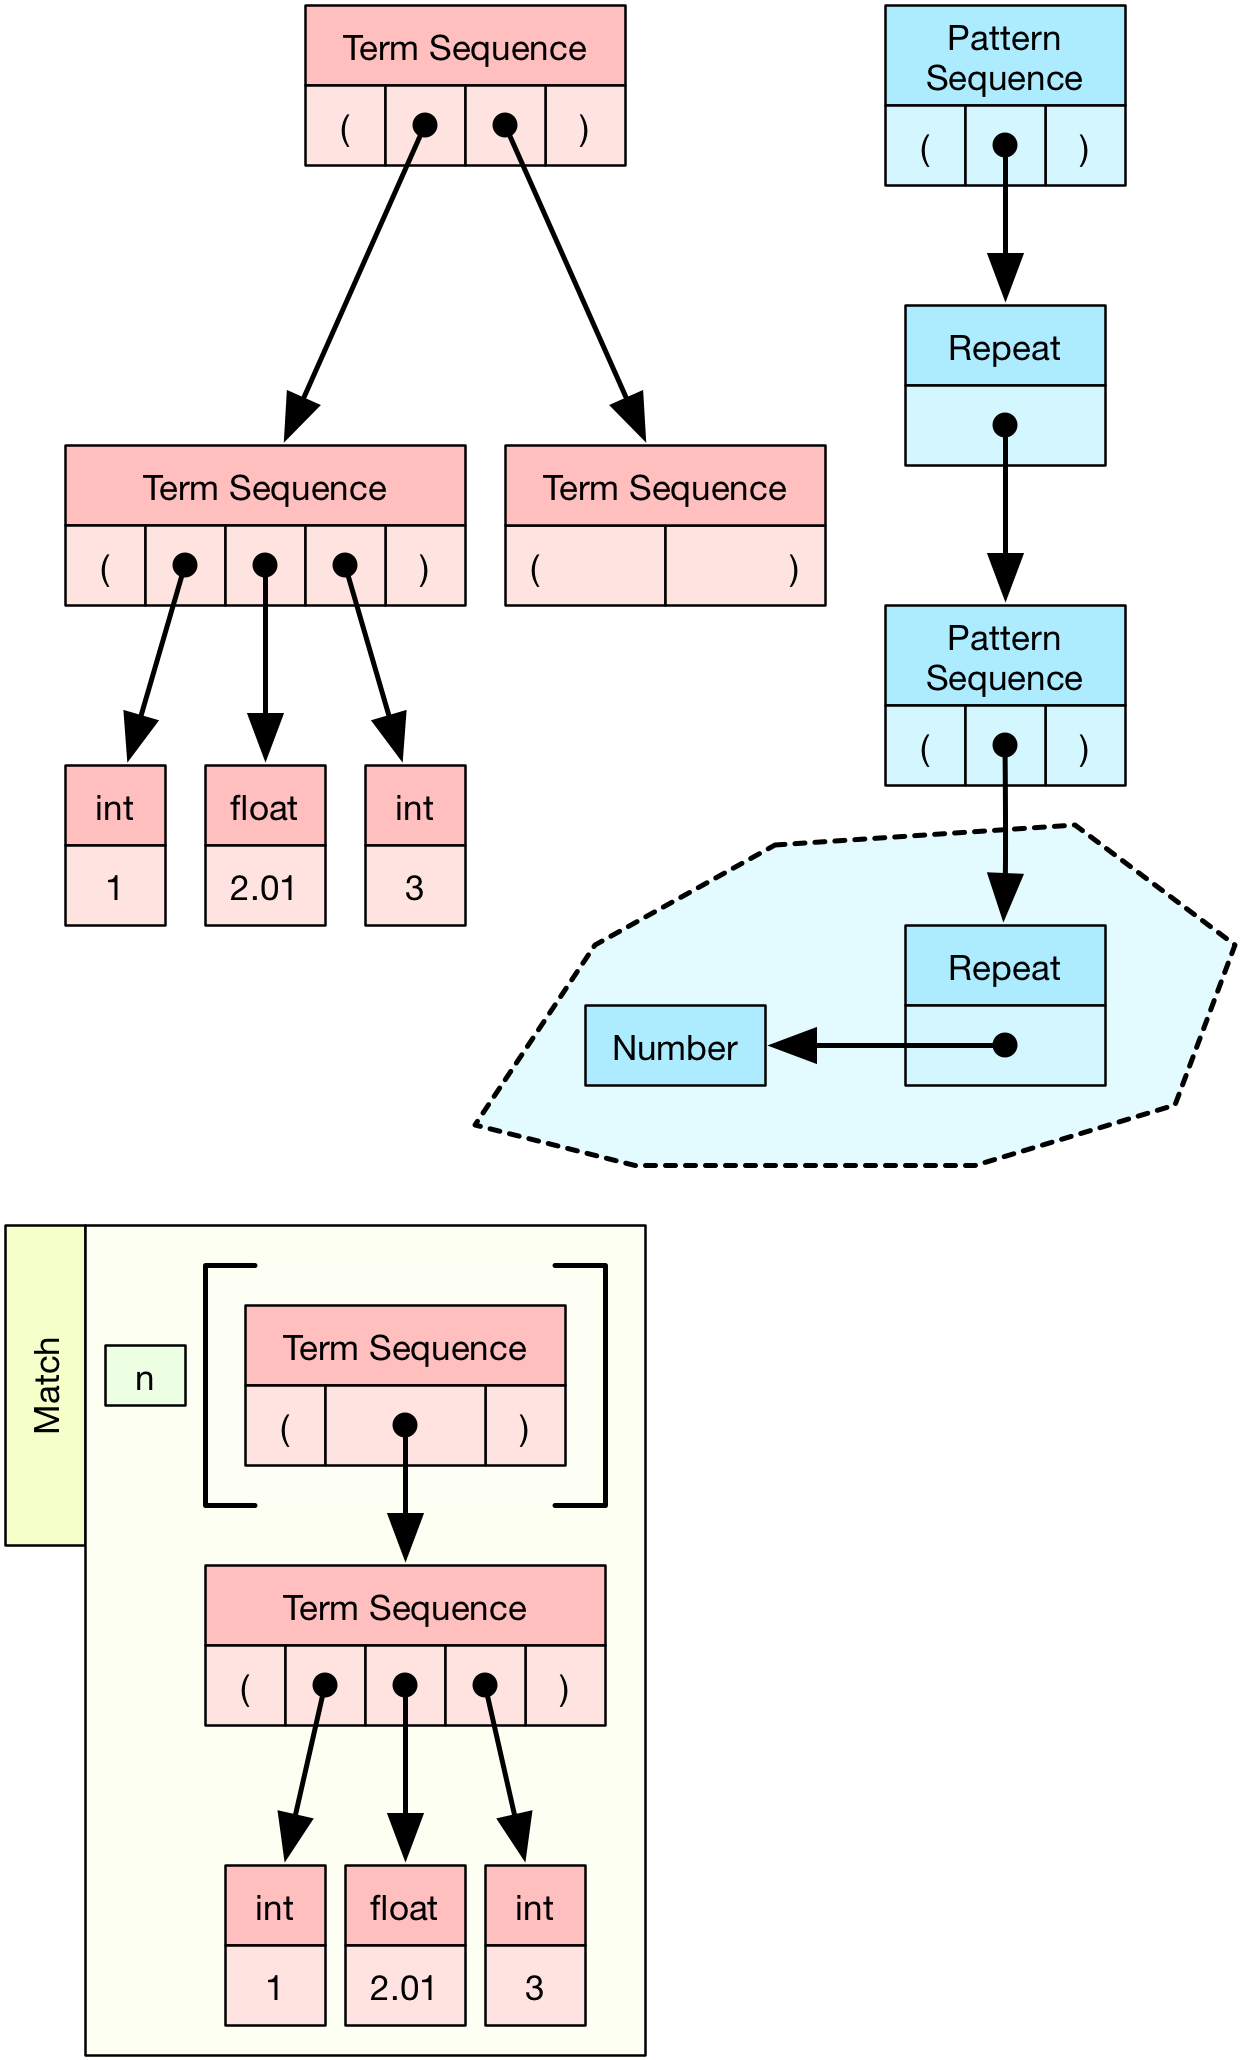
\includegraphics[scale=0.152]{ellipsis-example-fig-g.png}
		\caption{\texttt{decreasedepth("n")} and leave inner ellipsis.}
		\label{ellipsis-example-fig-g}
	\end{subfigure}
	\begin{subfigure}{0.5\linewidth}
		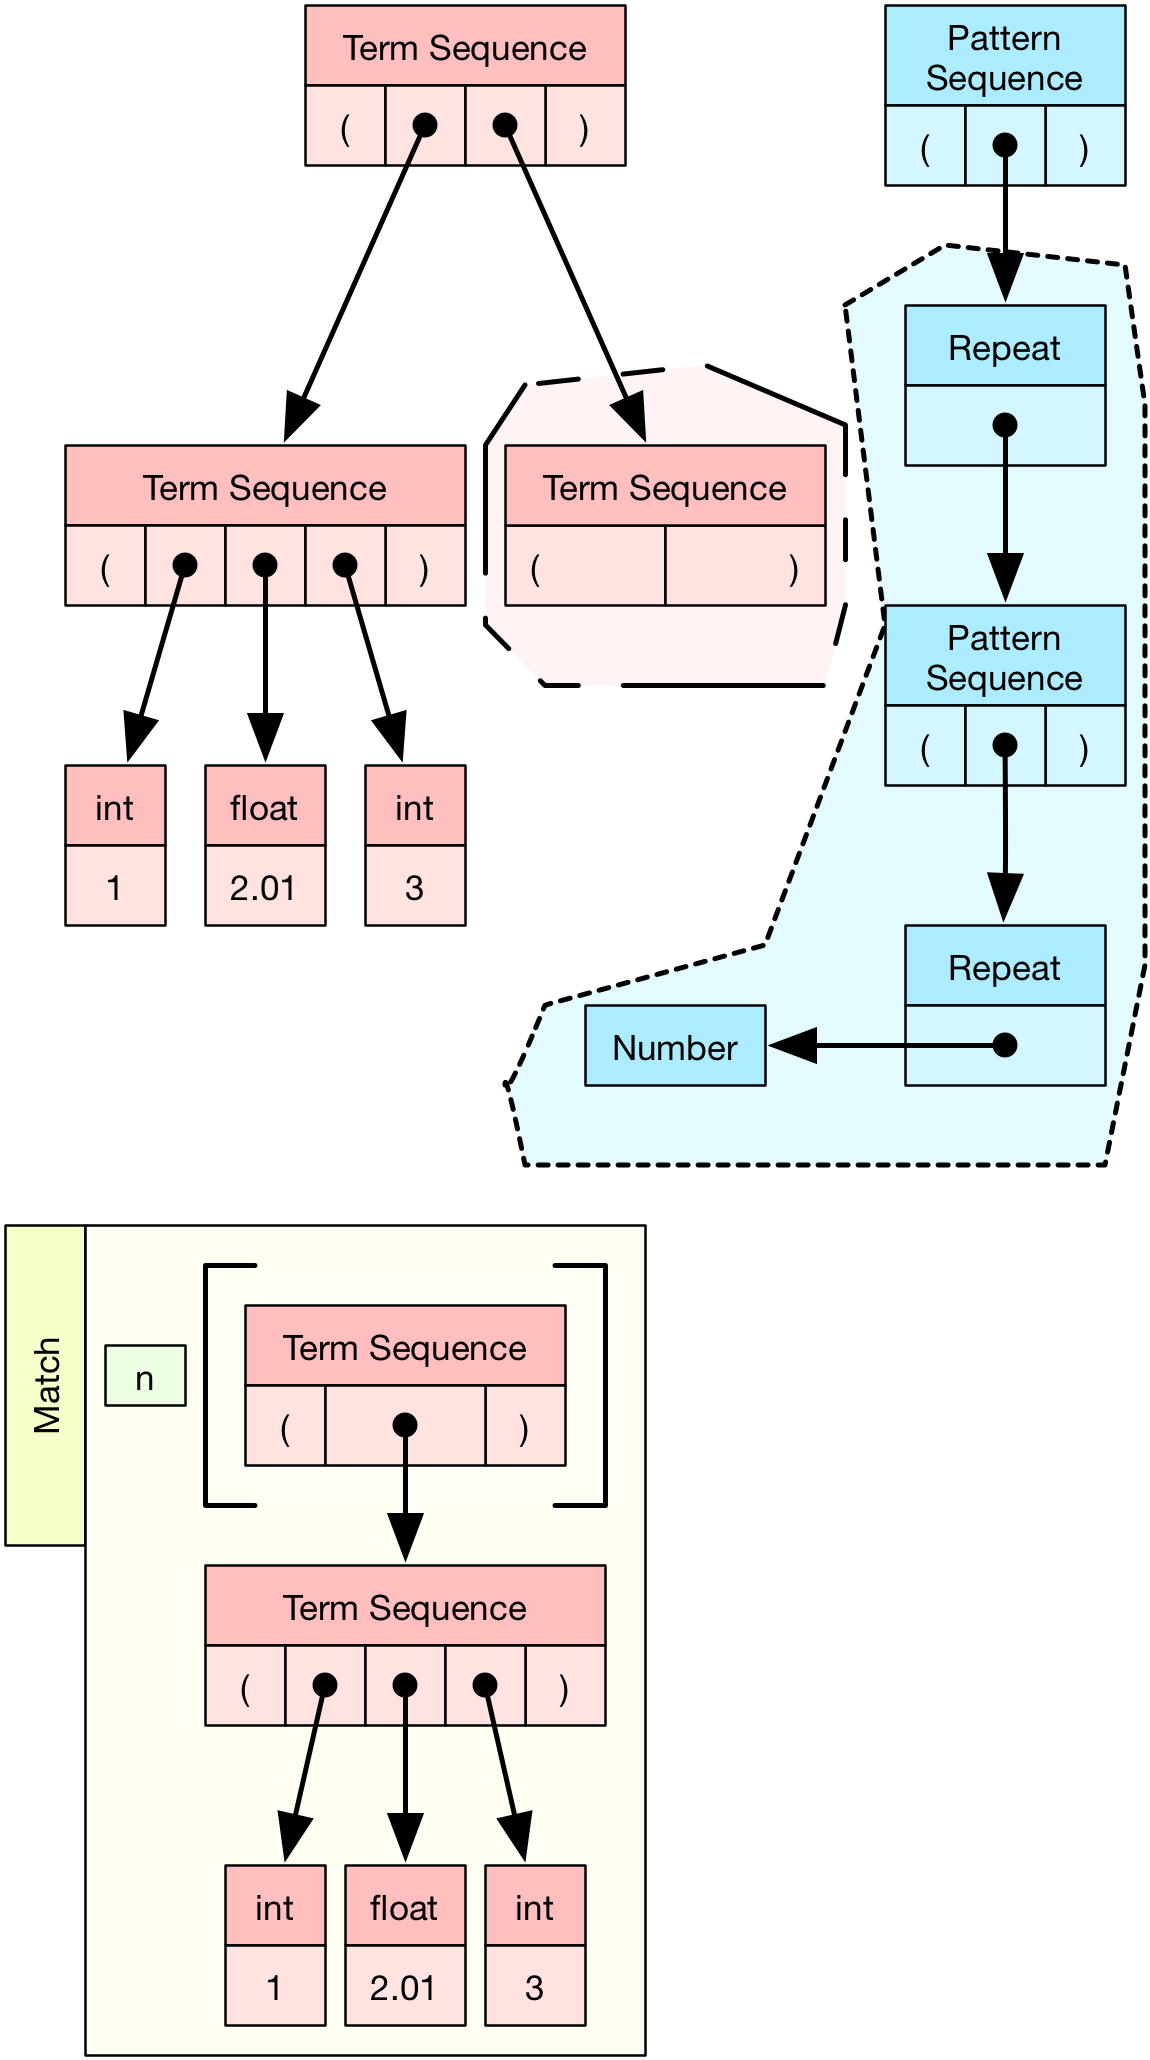
\includegraphics[scale=0.152]{ellipsis-example-fig-h.png}
		\caption{Start processing the next term in the sequence.}
		\label{ellipsis-example-fig-h}
	\end{subfigure}
	}
}
\end{figure}
\begin{figure}[H]\ContinuedFloat

\makebox[\textwidth][c] { 
	\fbox{
		\begin{subfigure}{0.5\linewidth}
			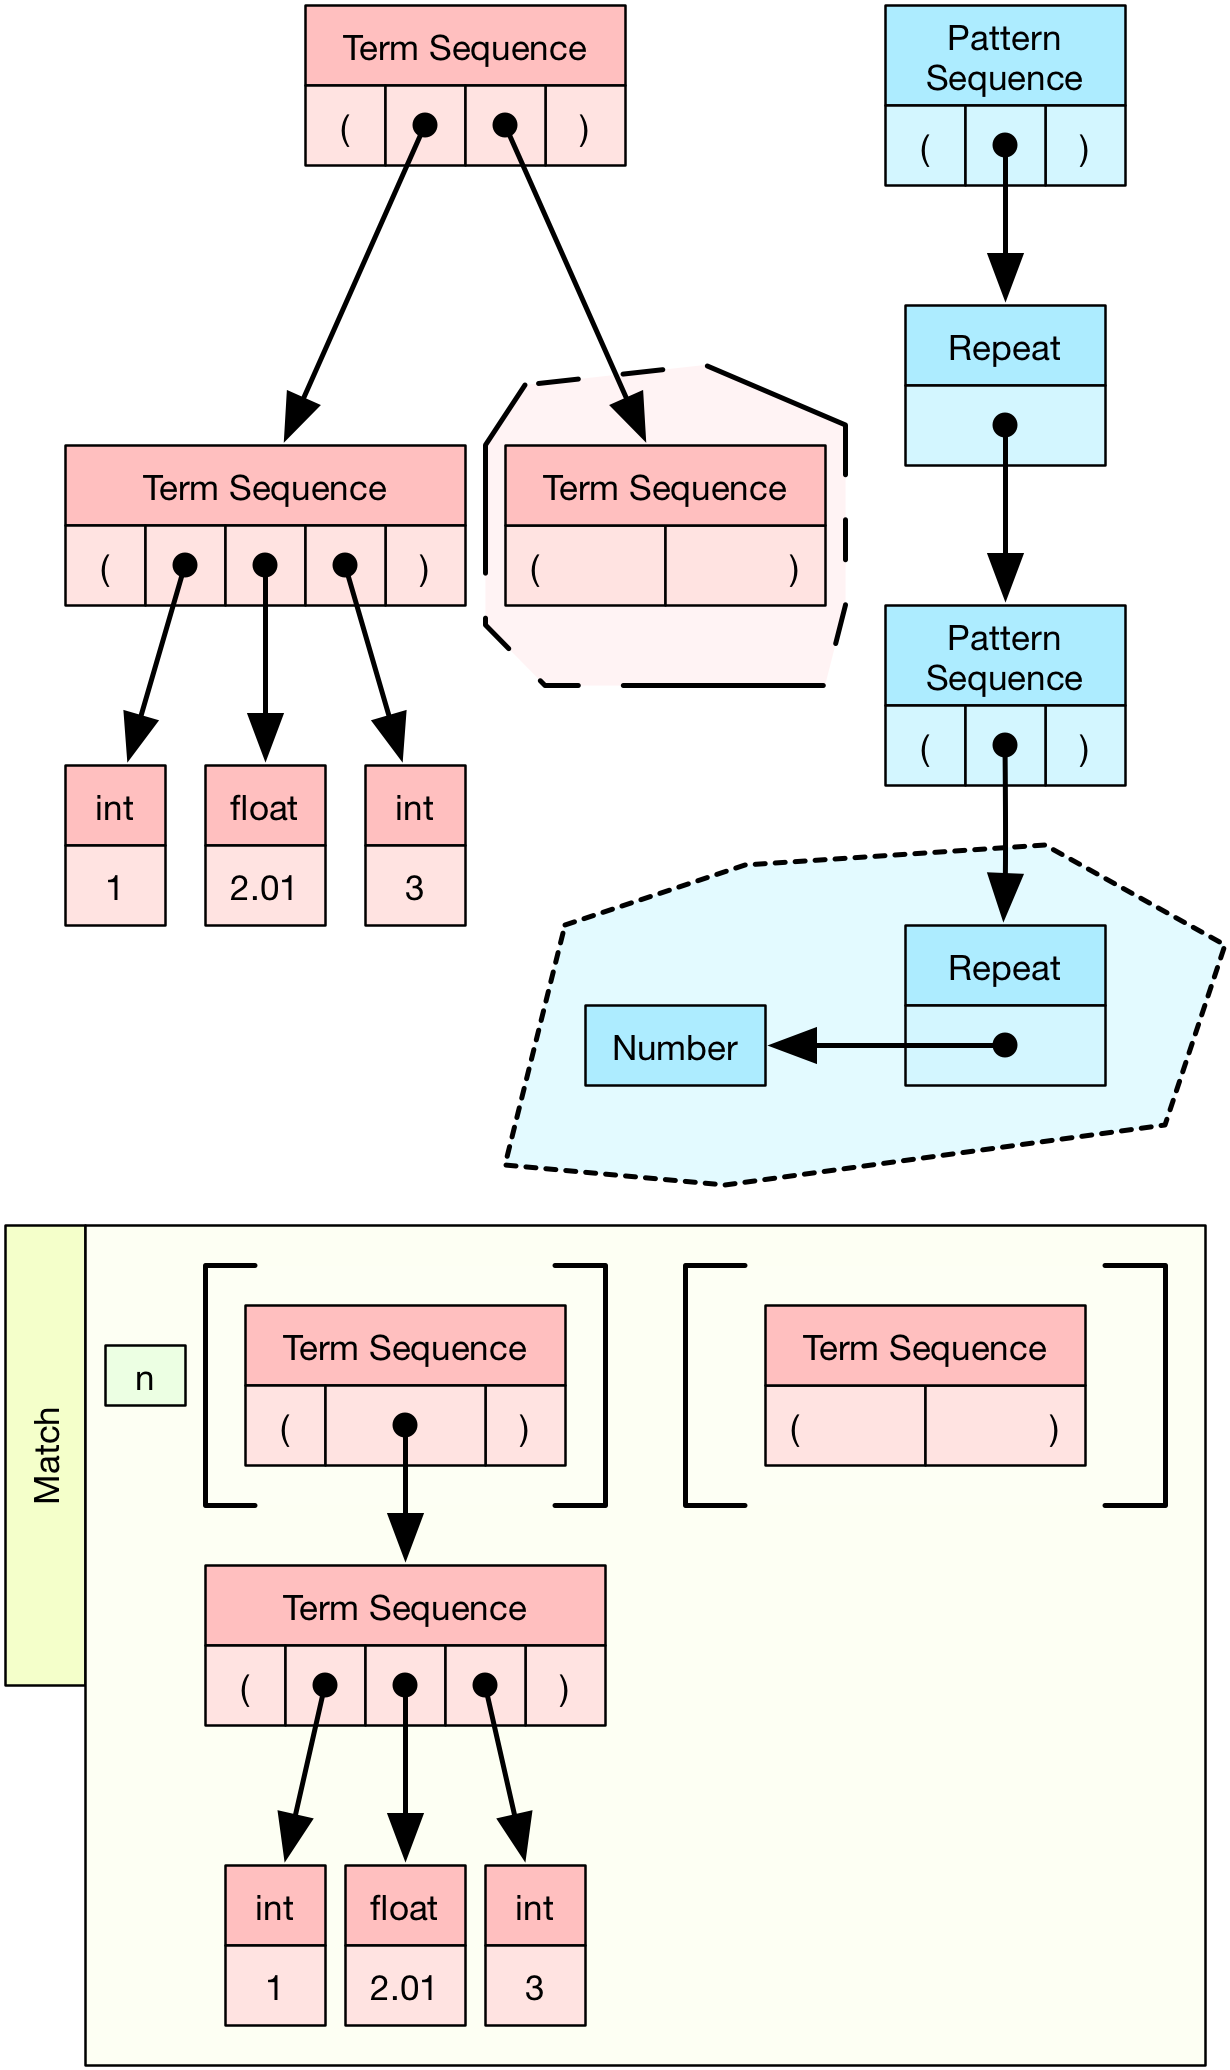
\includegraphics[scale=0.152]{ellipsis-example-fig-i.png}
			\caption{\texttt{increasedepth("n")} after entering inner ellipsis.}
			\label{ellipsis-example-fig-i}
		\end{subfigure}
		\begin{subfigure}{0.5\linewidth}
			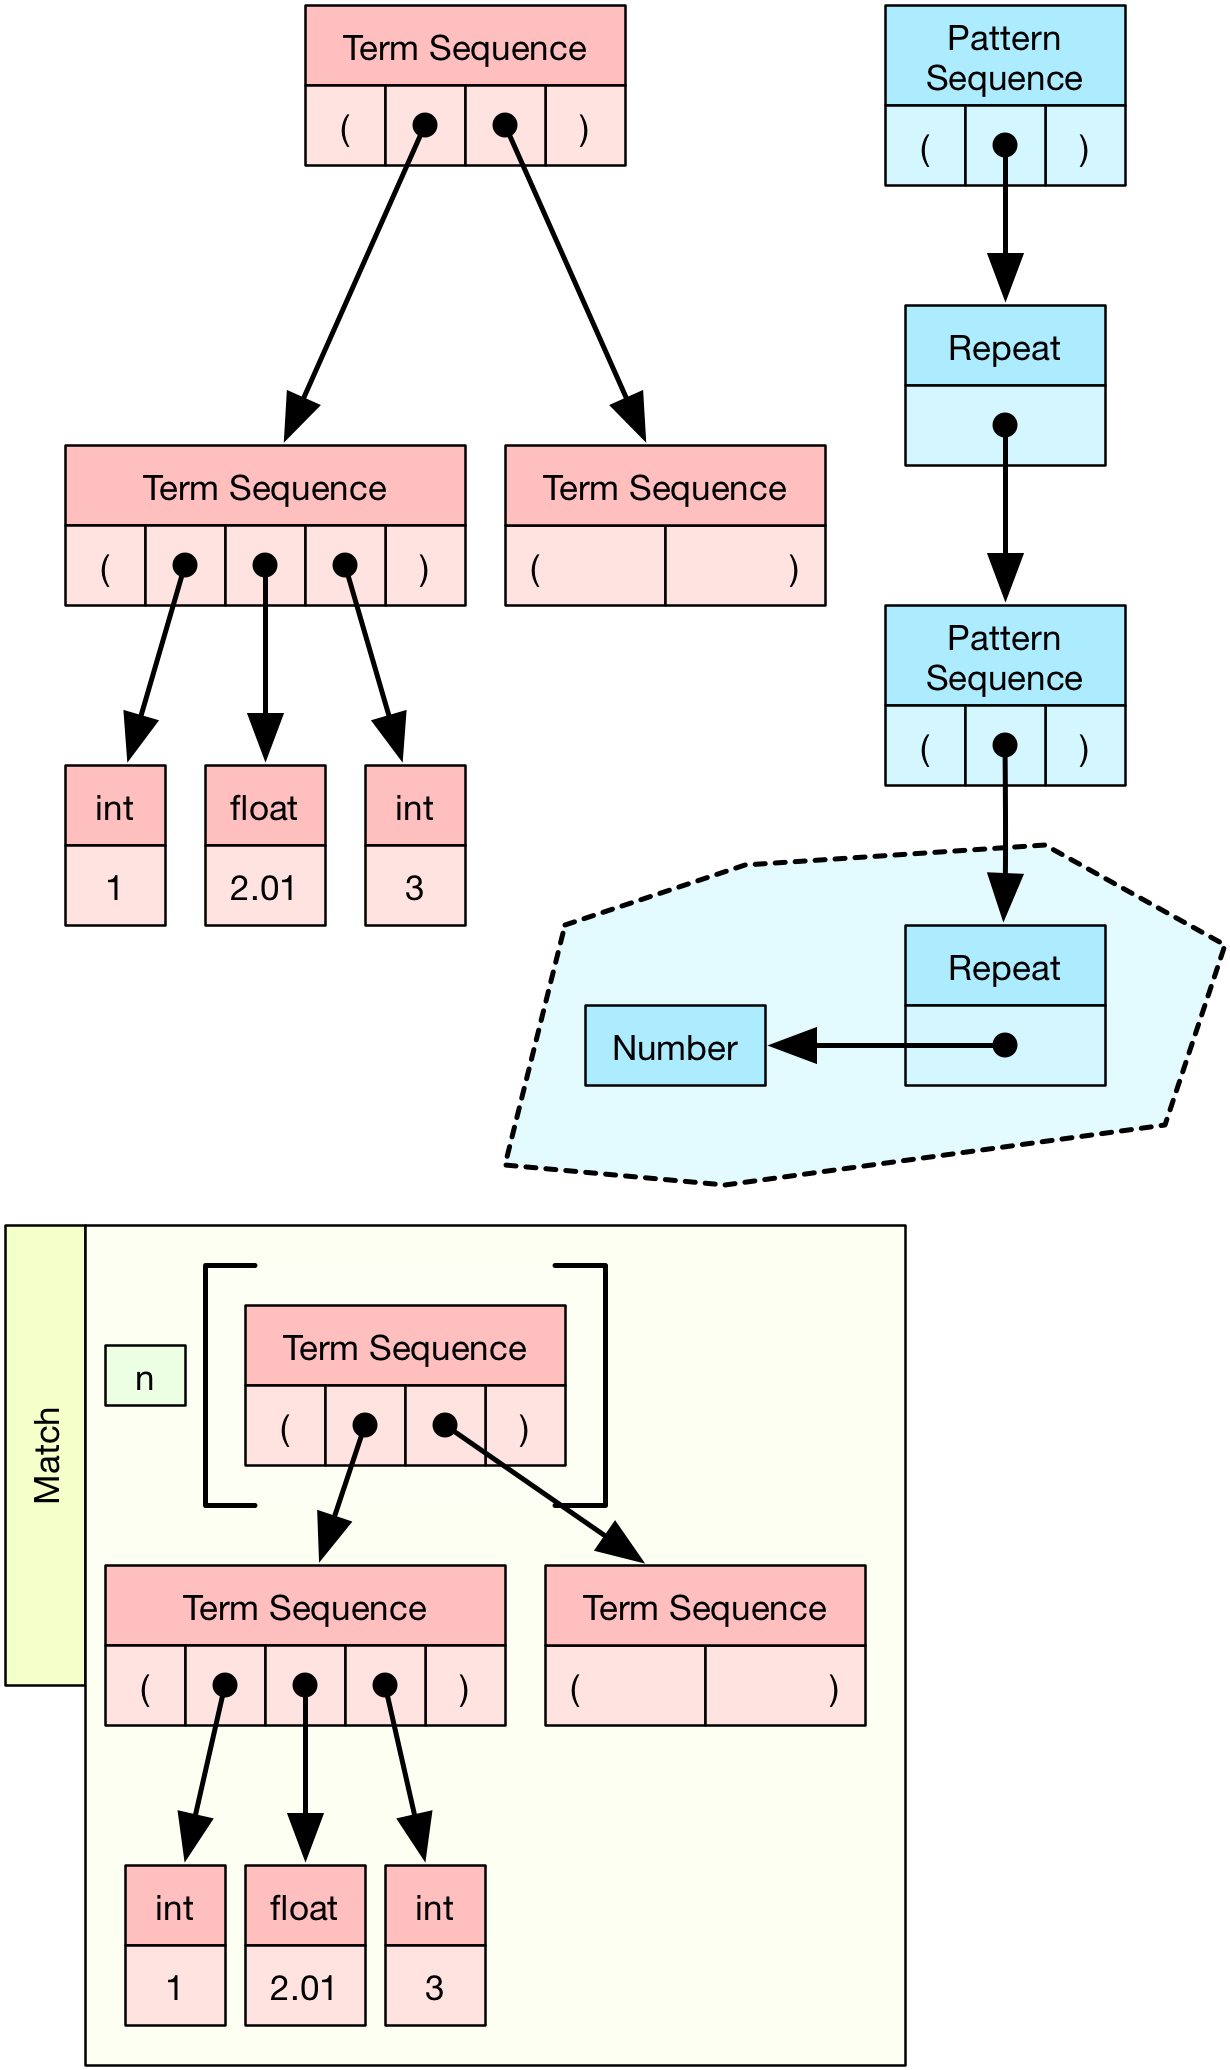
\includegraphics[scale=0.152]{ellipsis-example-fig-j.png}
			\caption{\texttt{decreasedepth("n")} and leave inner ellipsis.}
			\label{ellipsis-example-fig-j}
		\end{subfigure}
	}
}
\centering
\fbox{
	\begin{subfigure}{0.5\linewidth}
		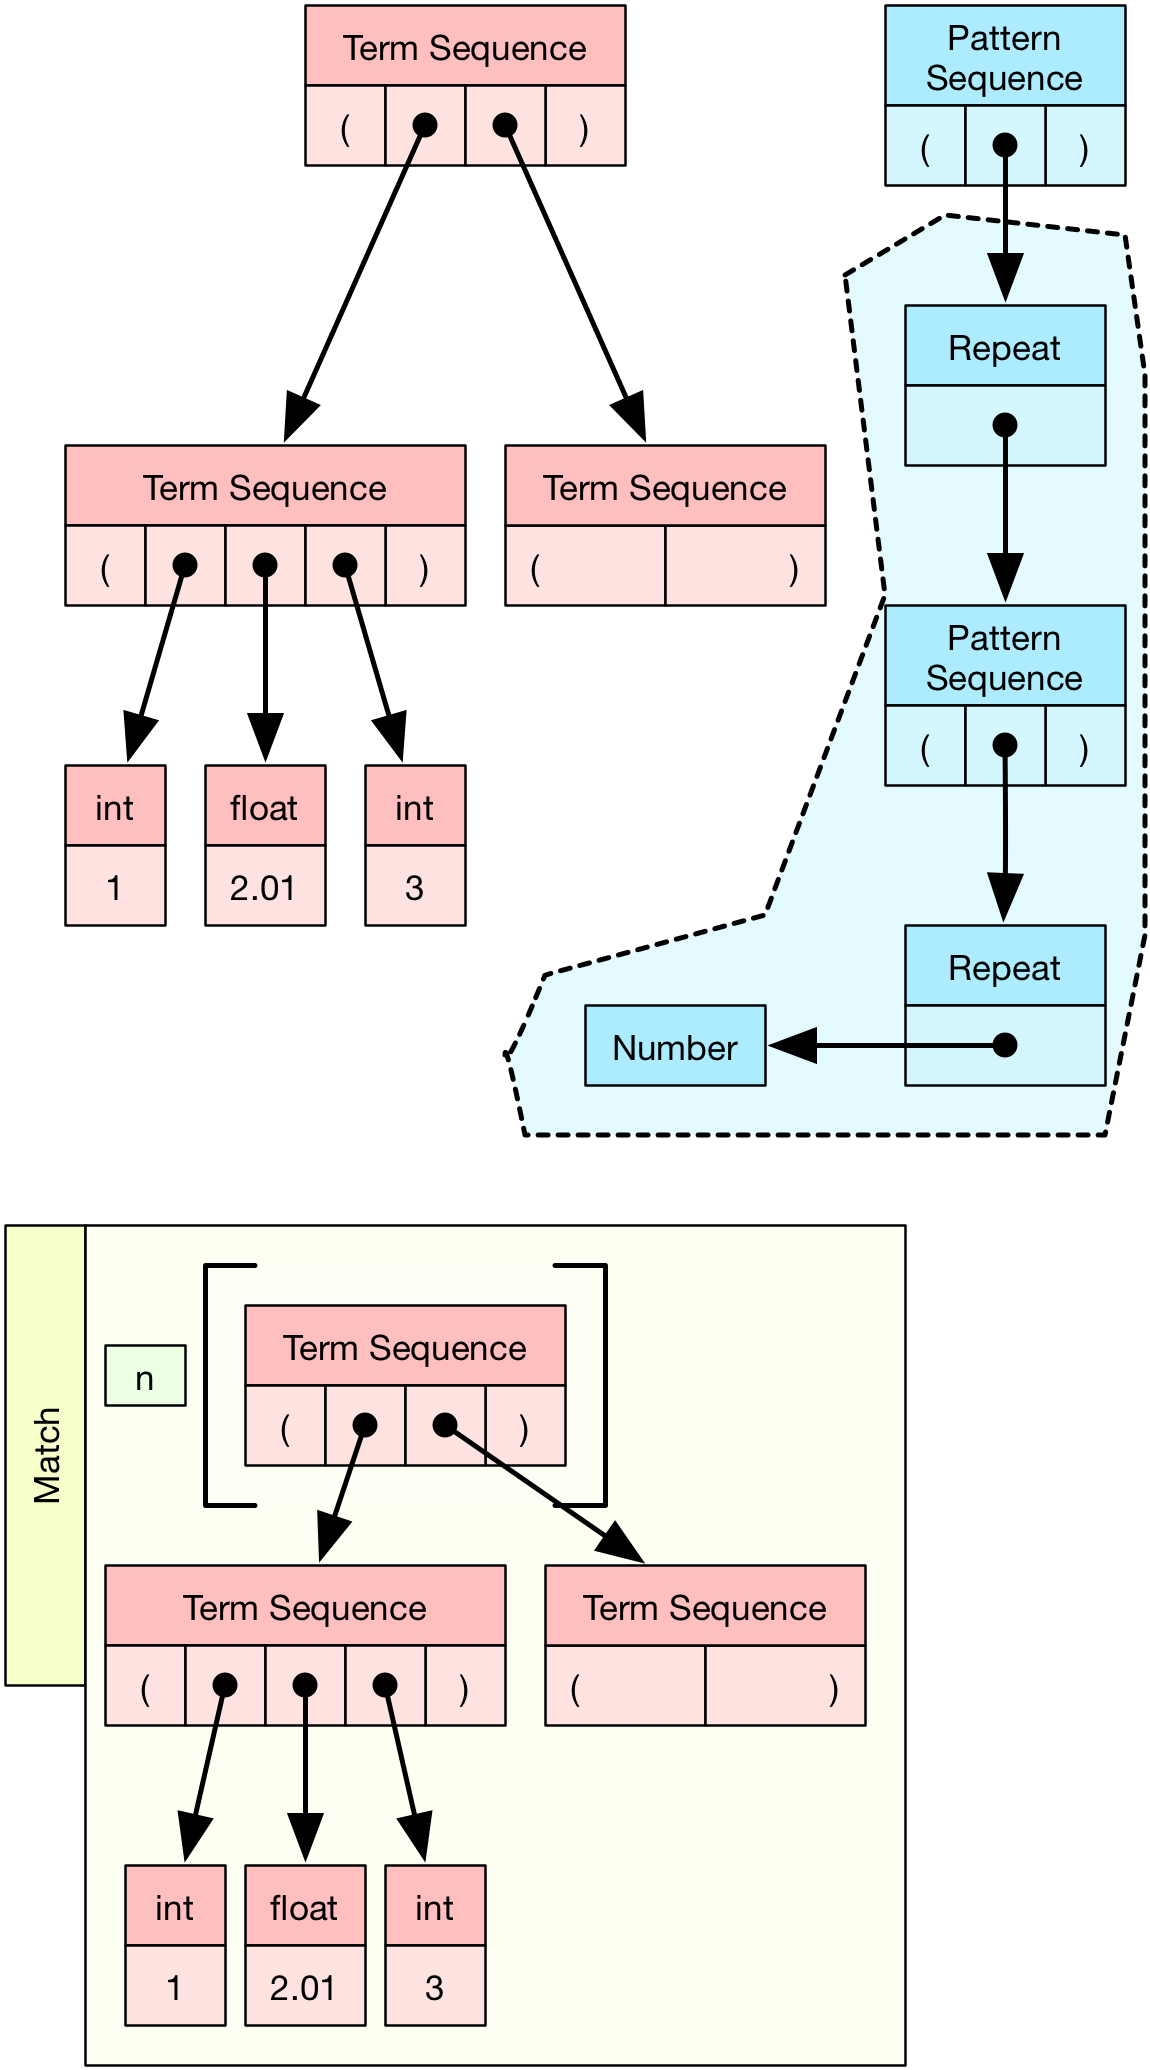
\includegraphics[scale=0.152]{ellipsis-example-fig-k.png}
		\caption{\texttt{decreasedepth("n") and leave outer ellipsis}.}
		\label{ellipsis-example-fig-k}
	\end{subfigure}
}

\end{figure}

\begin{figure}[H]
\centering
\makebox[\textwidth][c] { 
	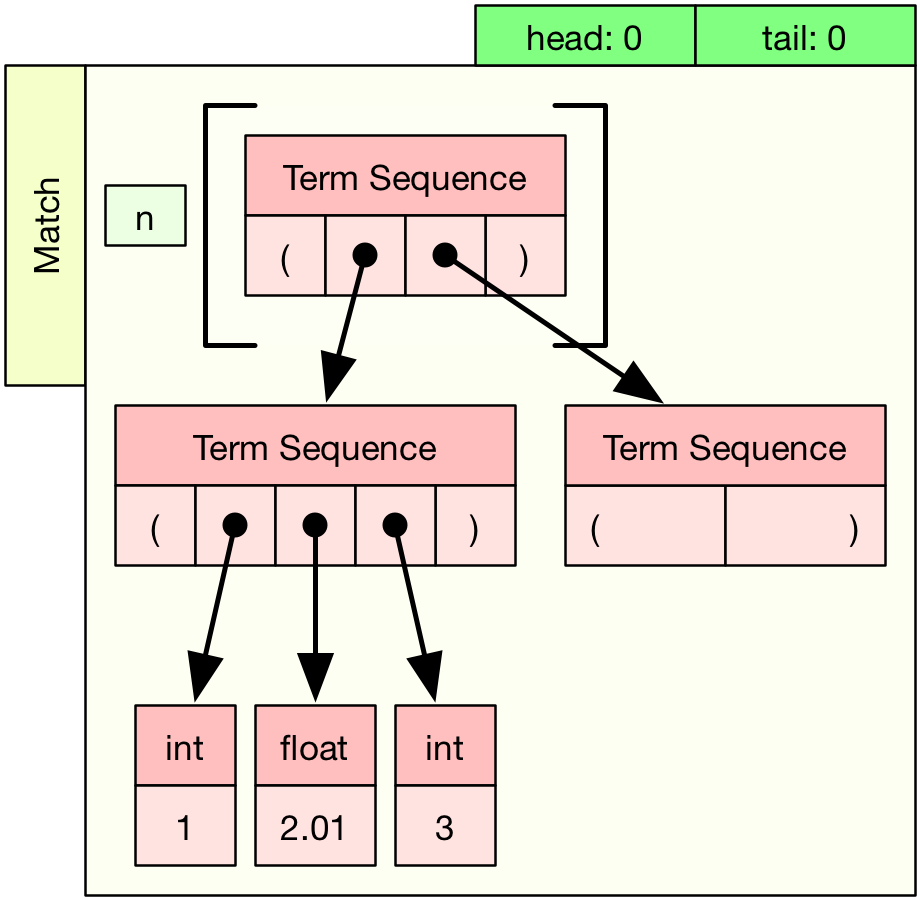
\includegraphics[scale=0.152]{ellipsis-example-matches-2.png}
}
\caption{Matches returned after matching term \texttt{()} against pattern \texttt{n ...}}
\label{ellipsis-example-matches-2}
\end{figure}

\begin{figure}[H]
\makebox[\textwidth][c] { 
	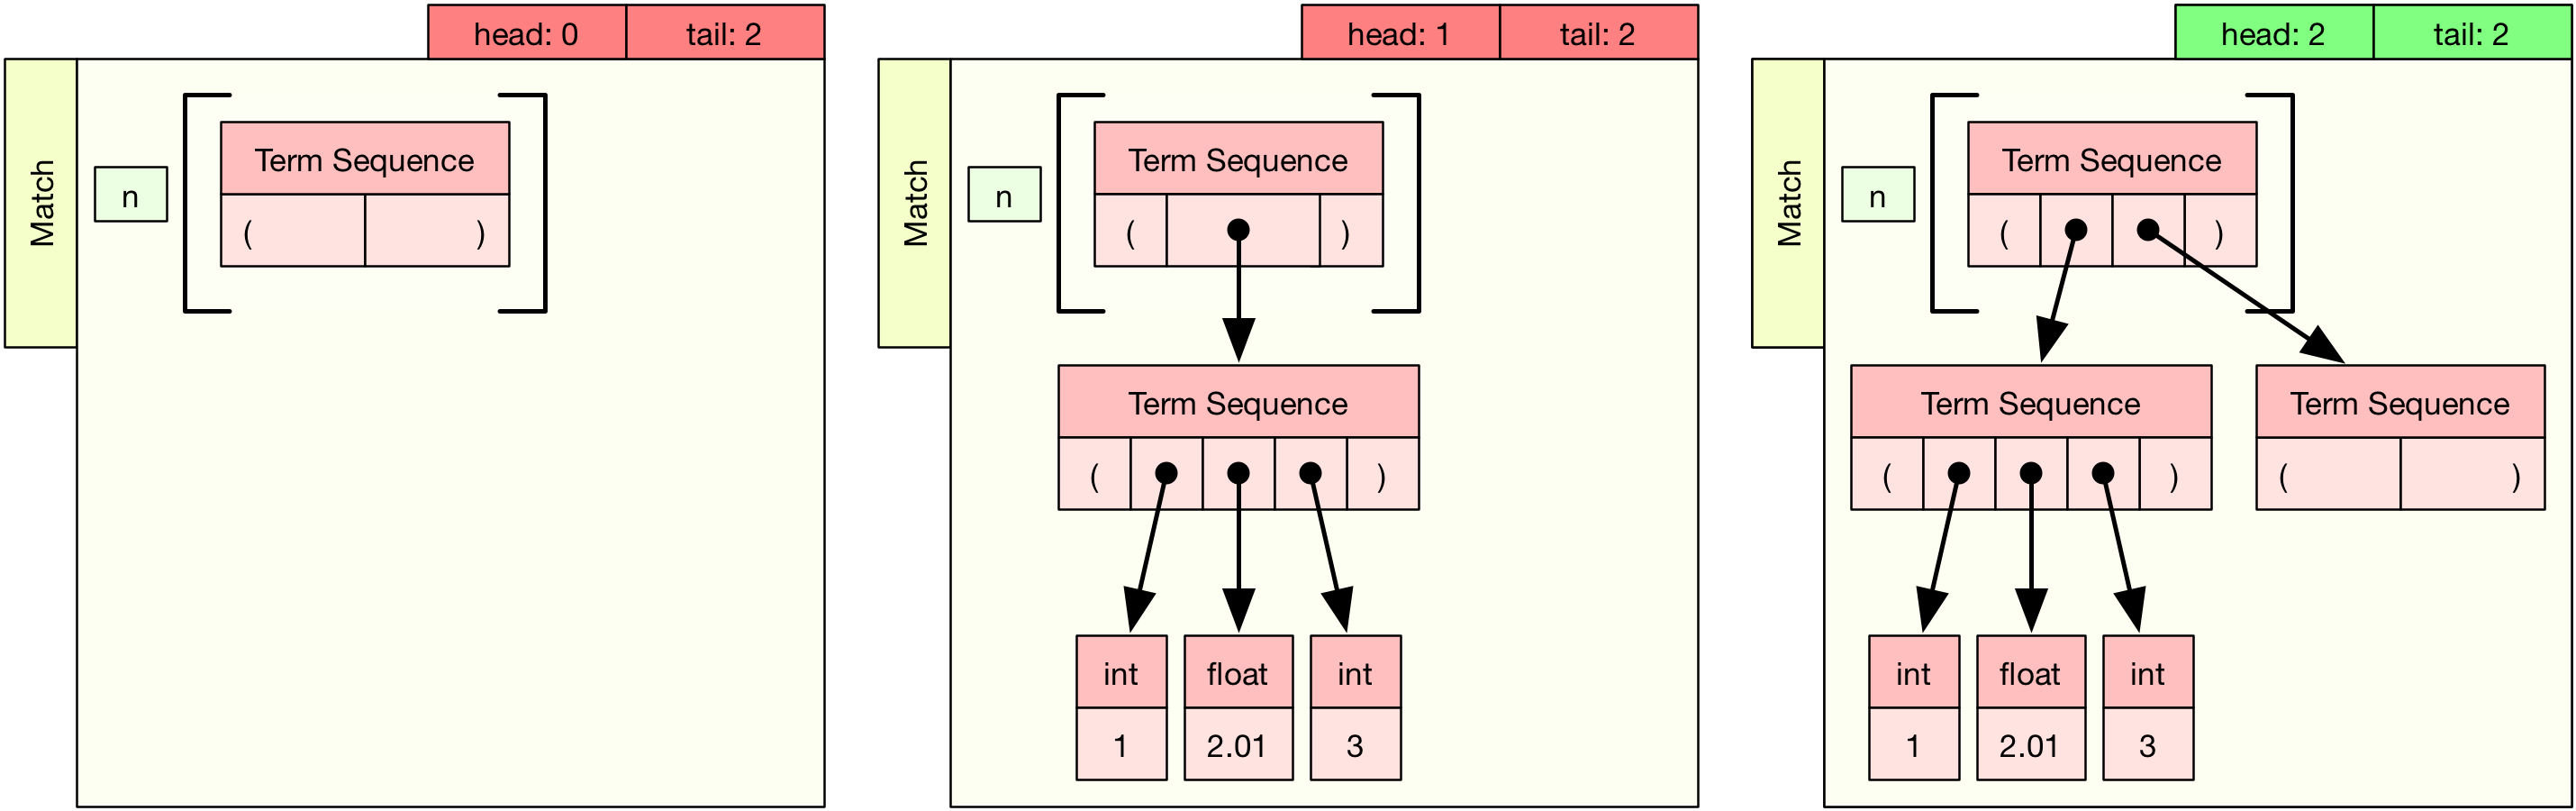
\includegraphics[scale=0.152]{ellipsis-example-matches-3.png}
}
\caption{Matches returned after matching term \texttt{((1 2 3)())} against pattern \texttt{(n ...) ...} }
\label{ellipsis-example-matches-3}
\end{figure}


\section{Term-Templates}

\subsection{Term Literals}

Given \TermLiteral, return the new term instance based on \texttt{TermLiteralKind}, as defined in Section \ref{section:term-templates}. Term-templates of this kind are guaranteed to not have \texttt{ForEach} and \texttt{InArg} annotations, by construction.

\begin{figure}[ht]
\begin{minted}[tabsize=2,obeytabs,escapeinside=||,mathescape=true,fontsize=\normalsize]{pythoncomplexer.py:PythonCompLexer -x}

	
def |$f_t$|(match):
	
	return Variable(|$v$|)
	
	return Integer(|$v$|)
	
	return Float(|$v$|)
	
	return String(|$v$|)
	
	return Boolean(|$v$|)
	
	return Hole()
	

\end{minted}
\caption{Code generation form literal terms.}
\label{codegen-term-template-lit}
\end{figure}

\subsection{Pattern Variables}

Given $t =$ \PatternVariable, let $f_t$ be a term-generating function for $t$. One of two scenarios may happen:
\begin{itemize}
\item $t$ has an \texttt{InArg(paramname)} annotation, meaning that this pattern-variable originally must have been under ellipsis.
\item $t$ has an \texttt{ReadMatch(pv, paramname)} annotation, meaning that this pattern-variable must not have been under an ellipsis. Simply return the term bound to pattern-variable $pv$.
\end{itemize}

\begin{figure}[htb]
\begin{minted}[tabsize=2,obeytabs,escapeinside=||,mathescape=true,fontsize=\normalsize]{pythoncomplexer.py:PythonCompLexer -x}

	
	
	
	
def |$f_t$|(match, |$arg_1$|):
	return |$arg_1$|
	
def |$f_t$|(match):
	return match.getbinding(|$rm_1[pv]$|)
	

\end{minted}
\caption{Code generation for pattern-variables.}
\label{codegen-term-pv}
\end{figure}

\subsection{TermSequence}

Given \TermSequence, recursively generate code for term-templates $t_i$, resulting in functions $f_{t_1},..., f_{t_n}$. Let $f_t$ be a term-generating function for $t$. Let $arg_1, ..., arg_n$ be a list of parameters to $f_t$, acquired by reading an \texttt{InArg} annotation. Let $mr_1, ..., mr_n$ be a list of \texttt{(id: str, s: str)} acquired by reading a \texttt{ReadMatch} annotation. For each such tuple, emit assignment to the metavariable \texttt{id} to the result of calling \texttt{match.getbinding(s)}.


\begin{figure}[ht]
\begin{minted}[tabsize=2,obeytabs,escapeinside=||,mathescape=true,fontsize=\normalsize]{pythoncomplexer.py:PythonCompLexer -x}

	
	
	
	
def |$f_t$|(match, |$arg_1, ..., arg_n$|):
	
	|$rm_i[id]$| = match.getbinding(|$rm_i[s]$|)
	
	sequence = Sequence()
	
		
		# snip
		
		# snip
		
		# snip
		
	return sequence
\end{minted}
\caption{Code generation for \TermSequenceNoArg.}
\label{codegen-term-sequence}
\end{figure}

Further code is generated based on the type of $t_i$. There are a few cases to consider.

\begin{itemize}
\item
The element is \TermRepeat. Retrieve the \texttt{ForEach} annotation and let $fe_1, ..., fe_n$ be the resulting set of pattern-variables. Note that these pattern-variables may be read from the match or simply passed as function parameters. First, ensure that the terms that are assigned to these pattern-variables are \texttt{Sequence} instances with equal lengths. An Exception is raised if the test fails. Otherwise, iterate over terms assigned to $fe_1, ..., fe_n$, retrieve the term at position $i$, and call $f_{t_i}$.

\begin{figure}
\begin{minted}[tabsize=2,obeytabs,escapeinside=||,mathescape=true,fontsize=\normalsize]{pythoncomplexer.py:PythonCompLexer -x}

lengths = set([])
	
	
assert isinstance(|$fe_i$|, Sequence)
lengths = lengths.union(|$fe_i$|.length())
assert len(lengths) == 1
	
for j in range(list(lengths)[0]): # convert set to list
	
	|$fe_i^{j}$| = |$fe_i$|.get(j)
	
	sequence.append(|$f_{t_i}$|(match, |$fe_1^{j}, ..., fe_n^{j}$|))
# snip
\end{minted}
\caption{Code generation for term-template \RepeatNoArg \space in \TermSequenceNoArg.}
\label{codegen-term-sequence-repeat}
\end{figure}

\item
	The element is \PythonCall. Call $f_{t_i}$ to obtain the term $t^{\prime}$. Notice that arguments for $f_{t_i}$ are generated using \texttt{InArg} annotations of $f_{t_i}$.
	\begin{enumerate}
	\item Insertion $mode$ is \texttt{Normal}. Append $t^{\prime}$ to the sequence.
	\item Insertion $mode$ is \texttt{Splice}. Ensure that $t^{\prime}$ is \texttt{Sequence} and then append each term in $t^{\prime}$ to the \texttt{term} \texttt{Sequence}.
	\end{enumerate}

\begin{figure}
\begin{minted}[tabsize=2,obeytabs,escapeinside=||,mathescape=true,fontsize=\normalsize]{pythoncomplexer.py:PythonCompLexer -x}

	|$t^{\prime}$| = |$f_{t_i}$|(match)
	
	sequence.append(|$t^{\prime}$|)
	
	assert isinstance(|$t^{\prime}$|, Sequence)
	for e in |$t^{\prime}$|:
		sequence.append(e)
	
#snip
\end{minted}
\caption{Code generation for term-template \PythonCallNoArg \space in \TermSequenceNoArg}
\label{codegen-term-sequence-pycall}
\end{figure}

\item Otherwise, simply call $f_{t_i}$ and append results to the sequence. Notice that the arguments for $f_{t_i}$ are generated using \texttt{InArg} annotations of $f_{t_i}$.

\begin{figure}
\begin{minted}[tabsize=2,obeytabs,escapeinside=||,mathescape=true,fontsize=\normalsize]{pythoncomplexer.py:PythonCompLexer -x}

	
t = |$f_{t_i}$|(match, |$a_1, ..., a_n$|)
sequence.append(t)

\end{minted}
\caption{Code generation for any other term-template in \TermSequenceNoArg}
\label{codegen-term-sequence-anyother}
\end{figure}
\end{itemize}

\subsection{Repeat}
Given \TermRepeat, generate the function $f_{t_r}$ for $t_r$. Since repetitions are handled in \TermSequenceNoArg, no special code generation is required here.

\subsection{InHole}
Given $t=$ \TermInHole, generate $f_{p_1}$ and $f_{p_2}$ for term-templates $p_1$ and $p_2$. Call $f_{p_1}$ and $f_{p_2}$ with appropriate arguments and then call the \texttt{plughole} function which is described in Section \ref{section:runtime-terms}.

\begin{figure}[htb]
\begin{minted}[tabsize=2,obeytabs,escapeinside=||,mathescape=true,fontsize=\normalsize]{pythoncomplexer.py:PythonCompLexer -x}

	
	
	
def |$f_t$|(match, |$arg_1, ..., arg_n$|):
	
	
	|$t_1^{\prime}$| = |$f_{t_1}$|(match, |$a_1, ..., a_n$|)
	|$t_2^{\prime}$| = |$f_{t_2}$|(match, |$b_1, ..., b_n$|)
	return plughole(|$t_1^{\prime}$|, |$t_2^{\prime}$|)
\end{minted}
\caption{Code generation for \PatternInHoleNoArg \space term-templates.}
\label{codegen-term-inhole}
\end{figure}


\subsection{PythonCall}
Given $t=$ \space \PythonCall \space, generate functions $f_1$, ..., $f_n$ for $t_1$, ..., $t_n$. Call procedures $f_{t_1}$, ..., $f_{t_n}$ with appropriate arguments and let $t_1^{\prime}$, ..., $t_n^{\prime}$ be the resulting terms. Call $pyfunc$ with the arguments $t_i^{\prime}$. Note that $t$ has neither \texttt{InArg} nor \texttt{MatchRead} annotations, by construction.

\begin{figure}[htb]
\begin{minted}[tabsize=2,obeytabs,escapeinside=||,mathescape=true,fontsize=\normalsize]{pythoncomplexer.py:PythonCompLexer -x}

	
	
def |$f_t$|(match):
	
	|$t_i^{\prime}$| = |$f_{t_i}$|(match)
	
	return |$pyfunc$|(|$t_1^{\prime},...,t_n^{\prime}$|)

\end{minted}
\caption{Code generation for \PythonCallNoArg \space term-templates.}
\label{codegen-term-pycall}
\end{figure}


\subsection{MetafunctionApplication}
The metafunction application is very similar to Python calls, except that there's only one term-template to be passed as an argument to the metafunction instead of many.

Given the term-template $t=$ \ApplyMetafunction, generate the function $f_t$ for $t$. Then, generate the function $f_{t_m}$ for term-template $t_m$. Call $f_{t_m}$ with the appropriate arguments, and feed results of $f$ into the metafunction with name $mf$.

\begin{figure}[htb]
\begin{minted}[tabsize=2,obeytabs,escapeinside=||,mathescape=true,fontsize=\normalsize]{pythoncomplexer.py:PythonCompLexer -x}

	
	
	
	
def |$f_t$|(match, |$arg_1, ..., arg_n$|):
	|$t_r^{\prime}$| = |$f_{t_r}$|(match, |$a_1, ..., a_n$|)
	return |$mf$|(|$t_r^{\prime}$|)

\end{minted}
\caption{Code generation for \MetafunctionApplicationNoArgs \space term-templates.}
\label{codegen-term-mfapply}
\end{figure}

\section{DefineLanguage Form}
Given \DefineLanguage, the only thing left to do here is to generate an \texttt{IsA} function for each $nt_i=$\space\NtDefinition:
\begin{enumerate}
\item Generate a matching function $f_{p_i}$ for pattern $p_i$ and let $f_{p_i}^{top}$ be the top-level matching function.
\item Call $f_{p_i}^{top}$ with \texttt{term} as an argument. If the resulting list of matches is non-empty, return True.
\item Otherwise, none of the patterns $p_i$ match the \texttt{term} and False is returned.
\end{enumerate}

Figure \ref{codegen-ntdef} demonstrates this.

\begin{figure}
\begin{minted}[tabsize=2,obeytabs,escapeinside=||,mathescape=true,fontsize=\normalsize]{pythoncomplexer.py:PythonCompLexer -x}

	
def |$f_{nt_i}$|(term):
	
		
	matches = |$f_{p_i}^{top}$|(term)
	if len(matches) > 0:
		return True
	
	return False
	

\end{minted}
\caption{Generation of \texttt{IsA} function for \NtDefinitionNoArgs.}
\label{codegen-ntdef}
\end{figure}

\section{DefineMetafunction Form}

Given $mf=$ \DefineMetafunction, generate a function $f_{mf}$ that accepts a single \texttt{Term} instance.

\begin{enumerate}
\item Generate matching functions $f_d$ for $domain$, $f_c$ for $codomain$ pattern, and let $f_d^{top}$, $f_c^{top}$ be top-level matching functions for $domain$ and $codomain$, respectively.
\item Code generation begins by calling $f_d^{top}$ with the term and ensuring that the resulting list of matches isn't empty, otherwise an Exception is raised.
\item For each $c_i =$ \MetafunctionCase[$p_i$][$t_i$], generate function $f_{c_i}$, passing the term as an argument.
\begin{enumerate}
	\item Generate the matching function $f_{p_i}$ for pattern $p_i$, and the term-creation function $f_{t_i}$ for term-template $t_i$. Let $f_{p_i}^{top}$ be top-level matching function for pattern $p_i$.
	\item Call $f_{p_i}^{top}$ with the term passed as argument. For each \texttt{match} in \texttt{matches}, call $f_{t_i}$ and if the result is not \texttt{None}, accumulate resulting terms into the list \texttt{terms}. If the resulting list \texttt{terms} is empty then return an empty list. Even though user-implemented Python functions are always expected to return a \texttt{Term} instance, since currently there's no support for \texttt{side-condition} clauses, returning \texttt{None} thus is the only way to "emulate" \texttt{side-condition} clauses.
	\item Ensure that all terms in \texttt{terms} are the same term. Metafunctions allow for non-deterministic behavior during pattern-matching but resulting \texttt{Match} instances must always produce the same term. Call function \newline \texttt{aretermsequalpairwise} with \texttt{terms} and raise an \texttt{Exception} if False is returned. Otherwise, pick any term from \texttt{terms}, and return it.
\end{enumerate}
\item If $f_{c_i}$ returns a term, call the $codomain$ function $f_c^{top}$ with the term as the argument. If the resulting list of matches is empty, then raise \texttt{Exception}, otherwise return the term. If metafunction-case function $f_{c_i}$ doesn't return anything, continue with next metafunction-case $f_{c_{i+1}}$
\item If after calling $f_{c_1}, ..., f_{c_n}$ no terms are returned, none of the metafunction cases were matches and an Exception is thrown.
\end{enumerate}

Code generated for \DefineMetafunctionNoArgs \space can be seen in Figure \ref{codegen-define-metafunc}.
\begin{figure}
\begin{minted}[tabsize=2,obeytabs,escapeinside=||,mathescape=true,fontsize=\normalsize]{pythoncomplexer.py:PythonCompLexer -x}

	
	
	
def |$f_{mf}$|(term):
	if len(|$f_d^{top}$|) == 0:
		raise Exception("domain check failed")
	
		
	nterm = |$f_{c_i}$|(term)
	if len(nterm) == 1:
		if len(|$f_c^{top}$|(nterm[0])) == 0:
			raise Exception("co-domain check failed")
		return nterm[0]
	
	raise Exception("no metafunction case matched")




	
	
	
def |$f_{c_i}$|(term):
	terms = []
	matches = |$f_{p_i}^{top}$|(term)
	for match in matches:
		if match is None: continue
		terms.append(|$f_{t_i}$|(match))
	if len(terms) == 0: return terms
	if not aretermsequalpairwise(term):
		raise Exception("produced multiple terms")
	return [terms[0]]


\end{minted}
\caption{Code generation for \DefineMetafunctionNoArgs.}
\label{codegen-define-metafunc}
\end{figure}

\section{DefineReductionRelation Form}
Given $red=$ \TlDefineReductionRelation, generate the function $f_{red}$ accepting a single term. The function returns a list of terms. The code generation algorithm works in the following manner:

\begin{enumerate}
\item Generate the top-level matching function $f_d^{top}$ for $domain$, if $domain$ is present, add call $f_d^{top}$ with \texttt{term}. If the resulting list of matches is empty, raise an Exception.
\item For each $r_i= $ \ReductionCase, generate function $f_{r_i}$.
	\begin{enumerate}
	\item Generate the top-level matching function $f_p^{top}$ for pattern $p$, and generate the function $f_t$ for the term-template $t$.
	\item Inside $f_{r_i}$, $f_p^{top}$(term) is called, and each match in the resulting list of matches is fed into $f_t$ resulting in a term. Apply $f_d$ to the term, and if the resulting list of matches is empty, raise Exception, otherwise append the term to list \texttt{terms}.
	\item Return \texttt{terms}
	\end{enumerate}
\item In $f_{red}$ create an empty list \texttt{outterms}. For each $r_i$ in $r_1, ..., r_n$, call appropriate $f_{r_i}$ and accumulate results into \texttt{outterms}.
\item Return \texttt{outterms}
\end{enumerate}

Code generated for \DefineReductionRelationNoArgs \space can be seen in Figure \ref{codegen-define-red}.

\begin{figure}
\begin{minted}[tabsize=2,obeytabs,escapeinside=||,mathescape=true,fontsize=\normalsize]{pythoncomplexer.py:PythonCompLexer -x}

	
	
def |$f_{mf}$|(term):
	outterms = []
	
		
	outterms = outterms + |$f_{r_i}$|(term)
	
	return outterms




	
	
	
def |$f_{r_i}$|(term):
	terms = []
	matches = |$f_{p}^{top}$|(term)
	for match in matches:
		t = |$f_{t}$|(match)
		if len(|$f_d^{top}$|(t)) == 0:
			raise Exception("term outside domain")
		terms.append(t)
	return terms


\end{minted}
\caption{Code generation for \DefineReductionRelationNoArgs.}
\label{codegen-define-red}
\end{figure}

\section{ReadFromStdinAndApplyReductionRelation Form}

Let $tl=$ \space\ReadFromStdinAndApplyReductionRelation. If $mf$ is present, let $f_{mf}$ be a previously generated Python function for metafunction with the name $mf$. Let $f_{red}$ be a previously generated Python function for \DefineReductionRelationNoArgs \space with a name $red$. 

\begin{enumerate}
\item Call the \texttt{read\_from\_stdin\_and\_parse} function to obtain an initial term $t$.
\item If $mf$ is present, construct a new \texttt{Sequence} $(f_{mf}, t)$ and apply $f_{mf}$ to it. The resulting term is stored in list $ts$.
\item Apply $f_{red}$ to all terms $t_i$ in $ts$ and store the results in the list $ts^{\prime}$.
\item Let $ts$ = $ts^{\prime}$ and repeat the previous step until $ts$ is empty.
\end{enumerate}

\begin{figure}
\begin{minted}[tabsize=2,obeytabs,escapeinside=||,mathescape=true,fontsize=\normalsize]{pythoncomplexer.py:PythonCompLexer -x}

	
	
	
def |$f_{tl}$|():
	|$t$| = read_from_stdin_and_parse()
	
	|$t$| = Sequence([|$f_{mf}$, $t$|])
	|$t$| = |$f_{mf}$|(|$t$|)
	
    |$ts$| = [|$t$|]
    while len(|$ts$|) != 0:
        |$ts^{\prime}$| = []
        for term in |$ts$|:
            terms = |$f_{red}$|(term)
            |$ts^{\prime}$|= |$ts^{\prime}$| + terms 
        |$ts$| = |$ts^{\prime}$|

\end{minted}
\caption{Code-generation for \ReadFromStdinAndApplyReductionRelationNoArgs \space form.}
\label{codegen-repl}
\end{figure}

\section{RedexMatchAssertEqual Form}
Given \RedexMatchAssertEqual, code generation proceeds in the following manner.

\begin{enumerate}
\item First, generate a list of expected matches \texttt{expectedmatches}. For each $m_i =$ \Match,
\begin{enumerate}
\item Generate the function $f_{t_i}$ for $t_i$ and let resulting the term be $tt_i = f_{t_i}(\texttt{Match()})$
\item Create an empty \texttt{Match} instance \texttt{match}, call \texttt{match.AddBinding}$(s_i)$ and \newline \texttt{match.AddToBinding}$(tt_i)$ methods, and then append \texttt{match} to \texttt{matches}.
\end{enumerate}
\item Generate the top-level matching function $f_p^{top}$ for pattern $p$ and the term-generating function $f_t$ for term-template $t$.
\item Let \texttt{actualmatches} = $f_p(f_t(\texttt{Match()}))$ and then call \texttt{assert\_compare\_match\_lists} with \texttt{expectedmatches} and \texttt{actualmatches}.
\end{enumerate}

\begin{figure}[h]
\begin{minted}[tabsize=2,obeytabs,escapeinside=||,mathescape=true,fontsize=\normalsize]{pythoncomplexer.py:PythonCompLexer -x}

	
		
			
def |$f_{rm}$|():
	
	|$mi_i$| = Match()
		
			
	term = |$f_{t_i}$|(Match())
	|$mi_i$|.addkey(|$s_i$|)
	|$mi_i$|.addbinding(|$s_i$|, term)
		
	
	expectedmatches = [|$mi_1, ..., mi_n$|]
	term = |$f_t$|(Match())
	actualmatches = |$f_p^{top}$|(term)
	assert_compare_match_lists(actualmatches, expectedmatches)


\end{minted}
\caption{Code generation for \RedexMatchAssertEqualNoArgs \space form.}
\label{codegen-redexmatch}
\end{figure}

\section{TermLetAssertEqual Form}

Given $tl=$ \TermLetAssertEqual, code generation proceeds in the following manner.
\begin{enumerate}
	\item First, produce the \texttt{Match} instance containing all pattern-variable $v_i$ assignments. Let $m=$ \texttt{Match()}. For each $(v_i, n_i, t_i)$
	\begin{enumerate}
	\item Generate the $f_{t_i}$ function for term $t_i$.
	\item $m$.\texttt{AddBinding}$(v_i)$ and $m$.\texttt{AddToBinding}$(v_i, f_{t_i}(\texttt{Match()}))$
	\end{enumerate}
\item Generate $f_t$ for term-template $t$ and $f_e$ for the term-template $e$.
\item Call \texttt{asserttermsequal}$(f_t(m), f_e(\texttt{\texttt{Match()}}))$.
\end{enumerate}

\begin{figure}[htb]
\begin{minted}[tabsize=2,obeytabs,escapeinside=||,mathescape=true,fontsize=\normalsize]{pythoncomplexer.py:PythonCompLexer -x}

	
	
	
def |$f_{tl}$|():
	match = Match()
	
		
	term = |$f_{t_i}$|(Match())
	match.addkey(|$v_i$|)
	match.addtobinding(|$v_i$|, term)
	
	expected = |$f_e$|(Match())
	actual = |$f_t$|(match)
	asserttermsequal(expected, actual)


\end{minted}
\caption{Code generation for \TermLetAssertEqualNoArgs \space form.}
\label{codegen-termlet}
\end{figure}


\section{ApplyReductionRelationAssertEqual Form}

Given \ApplyReductionRelationAssertEqual:
\begin{enumerate}
\item First, generate a list of expected terms \texttt{expected}, potentially empty.
	\begin{enumerate}
	\item Generate the function $f_{e_i}$ for each term-template $e_i$.
	\item Concatenate the results of $f_{e_i}(\texttt{Match()})$ to \texttt{expected}.
	\end{enumerate}
\item Generate the function $f_t$ for the term-template $t$.
\item Let $f_{red}$ be a Python function for \DefineReductionRelationNoArgs \space with the name $r$. Let \texttt{actual} = $f_{red}(f_t(\texttt{Match()}))$ be the list of terms after applying the reduction relation.
\item Call \texttt{asserttermlistsequal(expected, actual)}.
\end{enumerate}

\begin{figure}[htb]
\begin{minted}[tabsize=2,obeytabs,escapeinside=||,mathescape=true,fontsize=\normalsize]{pythoncomplexer.py:PythonCompLexer -x}

	
	
	
	
def |$f_{ar}$|():
	expected = [|$f_{e_1}(\texttt{Match()}), ..., f_{e_n}(\texttt{Match()})$|]
	actual = |$f_t$|(Match())
	asserttermlistsequal(expected, actual)


\end{minted}
\caption{Code generation for \ApplyReductionRelationAssertEqualNoArgs \space form.}
\label{codegen-applyred}
\end{figure}



\chapter{Testing and Evaluation}

\section{Testing}

To test PyPltRedex, two forms of testing are employed: 

\begin{enumerate}
\item Unit testing form most non-trivial transformation / analysis passes.
\item Integration tests containing \texttt{redex-match-assert-equal}, \texttt{term-let-assert-equal}, \texttt{apply-reduction-relation-assert-equal} forms that test functionality of pattern matching, term-generation and application of reduction relations and metafunctions. Some tests cases were lifted from a testing suite that comes with PLTRedex. All test cases use the output of PLTRedex for comparison.
\end{enumerate}

\section{Performance}

To get a feel for how PyPyPLTRedex would stack up against PLTRedex in terms performance, the Imp language was used to implement a simple iterative factorial calculator seen in Figure \ref{imp-factorial}. The program correctly computed factorial of 20 producing 2432902008176640000; factorial was evaluated 1000 times to obtain more reliable data. The program was also implemented in plain Python and compiled with the RPython toolchain. All programs were run three times and the resulting times were averaged. Results of profiling can be seen in Figure \ref{perf-fact}.

\begin{figure}[h]
\begin{minted}[tabsize=2,obeytabs,escapeinside=//,mathescape=true,fontsize=\normalsize]{python}
{
	(N = 20)
	(product = 1)
	(i = 1)
	[while (i <= N)
		(product = (product * i))
		(i = (i + 1))]
}
\end{minted}
\caption{Factorial program implemented in Imp.}
\label{imp-factorial}
\end{figure}

Benchmarking is set up in the way seen in Figure \ref{bench-setup}. Actual running time is measured with the utility \texttt{perf} and \texttt{chrt} is used to minimize context switches.

\begin{figure}[h]
\begin{minted}[tabsize=2,obeytabs,fontsize=\normalsize]{text}
sudo chrt -f 99 perf stat ./benc_fact/fact-c 
\end{minted}
\caption{Benchmarking setup.}
\label{bench-setup}
\end{figure}


\begin{figure}[h]
\centering
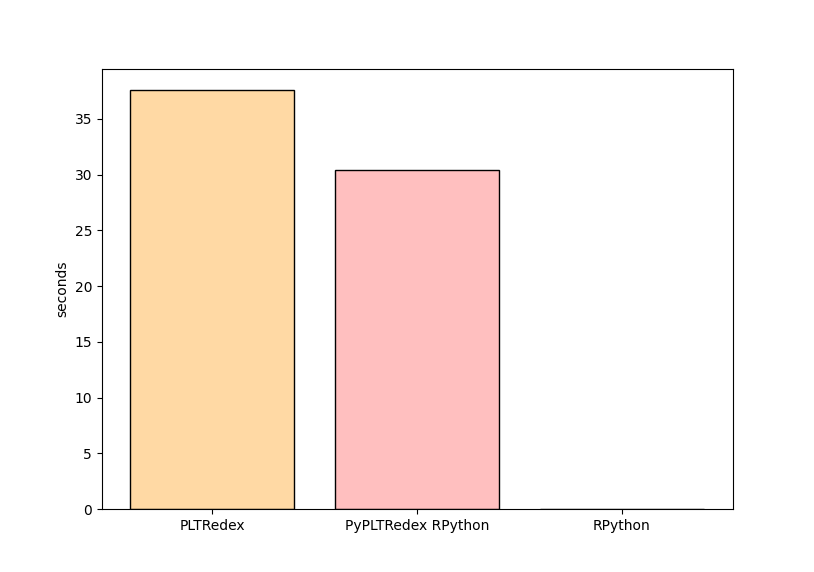
\includegraphics[scale=0.7]{perf-fact.png}
\caption{Profiling \texttt{Factorial(20)} program.}
\label{perf-fact}
\end{figure}

\chapter{Conclusion} 

\section{Future Work}
\subsection{Ellipsis Determinism}
In Chapter < Pattern codegen > an algorithm for deterministic matching of patterns under ellipsis was described but careful reader might notice the report doesn't describe how such patterns are made deterministic. In fact, PyPltRedex provides a transformation pass called \texttt{EllipsisMatchModeRewriter} that analyzes patterns under ellipses and decides if given ellipsis can be matched deterministically but current algorithm is flawed and doesn't work correctly for all patterns. 


\subsection{\texttt{define-metafunction} and \texttt{define-reduction-relation} pattern merging.}

Algorithms for application of reduction-relation and metafunctions match each pattern separately. However, it may be the case that patterns in reduction-cases are similar and bind terms to same identifiers in the same position within the pattern.

\begin{lstlisting}
(M_1  (in-hole P x (+ n_1 n_2)))
(M_1  (in-hole P n (- n_1 n_2)))
\end{lstlisting}

Two patterns above are an example - both patterns contain pattern-variable $M\_1$ in the first position within the sequence. This means at this point there needs to be a single $Match$ object containing $M\_1$. Since $in-hole$ patterns are different, after matching $M\_1$ $Match$ object can be copied to contain terms matches by each $in-hole$. Diagram can be seen below - 

TODO


Furthermore, the first pattern in both \texttt{in-hole} patterns is the same - $P$. Since both \texttt{in-hole} patterns are at the second position within respective pattern sequences, instead of using multiple term traversals to find child terms matching \texttt{(+ n\_1 n\_2)} and \texttt{(- n\_1 n\_2)}, one travesal would be sufficient. This could be done by introducing a new pattern, say, $InHoleMulti(pattern1, pattern2 ...)$ that accepts multiple patterns. Diagram for this can be seen below:

TODO


However, since since matches may have been split before, this introduces additional complexity of \texttt{Match} object management.

\subsection{More evaluation}

I was not able to explore performance of the system w.r.t. larger terms.


%\appendix 
%\input{appendix/pypltredex-source.tex}


\backmatter

%\bibliographystyle{alpha}
%\bibliographystyle{dcu}
\bibliographystyle{unsrt}
\bibliography{biblio}

%\cleardoublepage
%\theindex %optional, use only if you have an index, must use
	  %\makeindex in the preamble

\end{document}
